\newpage
\begin{center}
    \textbf{BAB IV} \\
    \textbf{HASIL DAN PEMBAHASAN}
    \addcontentsline{toc}{chapter}{BAB IV. HASIL DAN PEMBAHASAN}
\end{center}

\textbf{A. Data Uji Coba}
\addcontentsline{toc}{section}{A. Data Uji Coba}

\hspace*{1cm}Data uji coba dalam pengembangan media pembelajaran berbasis simulasi 3D pada materi bangun ruang untuk peserta didik kelas VIII SMP diperoleh melalui model pengembangan ADDIE. Tahapan pengembangan meliputi Analisis, Perancangan, Pengembangan, Implementasi, dan Evaluasi.

\begin{enumerate}[leftmargin=1cm, label=\arabic*.]
    \item \textbf{Analisis}
    
    \hspace*{1cm}Tahap analisis merupakan tahap awal dalam pengembangan. Peneliti melakukan analisis di SMP Muhammadiyah 9 Yogyakarta untuk memperoleh gambaran tentang media pembelajaran yang akan dikembangkan. Adapun analisis yang dilakukan meliputi:
    
    \begin{enumerate}[label=\textbf{\alph*.}]
        \item \textbf{Analisis Kebutuhan}
        
        \hspace*{1cm}Peneliti melakukan wawancara dengan guru matematika pada tanggal 28 April 2026 serta menyebarkan angket kepada peserta didik kelas VIII-B SMP Muhammadiyah 9 Yogyakarta. Hasil penyebaran angket pra-penelitian disajikan pada Tabel~\ref{pra-penelitian}.
        
        \begin{table}[H]
            \centering
            \caption{Hasil penyebaran angket Pra-Penelitian Peserta Didik}
            \label{pra-penelitian}
            \begin{tabular}{|c|p{6cm}|>{\centering\arraybackslash}p{1.5cm}|>{\centering\arraybackslash}p{1.5cm}|}
                \hline
                \multirow{2}{*}{No} & \multirow{2}{*}{Indikator} & \multicolumn{2}{c|}{Respons Peserta Didik} \\
                \cline{3-4}
                & & Ya & Tidak \\
                \hline
                1 & Apakah pelajaran matematika sulit? & 84,4\% & 15,6\% \\
                \hline
                2 & Apakah materi bangun ruang sisi datar sulit dipahami? & 75\% & 25\% \\
                \hline
                3 & Saya lebih tertarik dengan pembelajaran praktik, daripada hanya dijelaskan oleh guru. & 62,5\% & 37,5\% \\
                \hline
                4 & Saya menyukai pendekatan pembelajaran yang membuat peserta didik menjadi lebih aktif. & 93,75\% & 6,25\% \\
                \hline
                5 & Saya menyukai pembelajaran dengan menggunakan teknologi. & 87,5\% & 12,5\% \\
                \hline
            \end{tabular}
        \end{table}

        \hspace*{1cm}Berdasarkan Tabel \ref{pra-penelitian}, sebanyak 83,3\% peserta didik menganggap matematika sulit. Setelah penyebaran angket, peneliti juga melakukan wawancara kepada beberapa peserta didik. Hasil wawancara menunjukkan bahwa peserta didik mengalami kesulitan dalam menyelesaikan soal yang berkaitan dengan bangun ruang sisi datar, terutama karena kesulitan membayangkan bentuk bangun ruang tersebut. Hasil penyebaran angket dan wawancara dirangkum sebagai berikut.

        \begin{enumerate}
            \item Sumber belajar yang digunakan adalah buku LKS serta catatan dari guru.
            \item Model pembelajaran yang digunakan adalah metode ceramah dan tanya jawab.
            \item Peserta didik mengalami kesulitan dalam memahami materi bangun ruang sisi datar.
            \item Peserta didik menyukai pembelajaran yang memanfaatkan teknologi.
            \item Pendidik matematika kelas VIII-B SMP Muhammadiyah 9 Yogyakarta belum pernah menggunakan teknologi simulasi 3D dalam proses pembelajaran.
        \end{enumerate}

        \hspace*{1cm}Berdasarkan permasalahan tersebut, peneliti berniat menguji kelayakan media pembelajaran berbasis simulasi 3D untuk meningkatkan ketertarikan dan membantu pemahaman peserta didik terhadap materi bangun ruang sisi datar.

        \item \textbf{Analisis Materi}
        
        \hspace*{1cm}Berdasarkan hasil wawancara dengan pendidik matematika di SMP Muhammadiyah 9 Yogyakarta, peneliti menentukan materi Bangun Ruang Sisi Datar sebagai fokus pengembangan. Materi ini dinilai sulit oleh peserta didik, terutama dalam menyelesaikan soal gambar bangun ruang dan soal cerita, sehingga cocok dikembangkan dengan teknologi simulasi 3D.

        \item \textbf{Analisis Kurikulum}
        
        \hspace*{1cm}SMP Muhammadiyah 9 Yogyakarta menerapkan Kurikulum Merdeka. Oleh karena itu, materi pembelajaran dikembangkan sesuai dengan capaian pembelajaran Fase D untuk kompetensi geometri.

        \hspace*{1cm}Capaian pembelajaran Fase D pada domain geometri yang menjadi acuan pengembangan meliputi:
        \begin{enumerate}[label=\alph*)]
            \item Mengidentifikasi dan menganalisis sifat serta hubungan antar unsur bangun ruang sisi datar dan jaring-jaringnya.
            \item Menggunakan representasi visual, berupa gambar, model, dan simulasi, untuk memahami konsep bangun ruang.
            \item Menyelesaikan masalah kontekstual yang berkaitan dengan bangun ruang sisi datar menggunakan penalaran matematika.
            \item Mengkomunikasikan penjelasan matematis secara lisan atau tertulis terkait konsep dan proses penyelesaian masalah geometri.
        \end{enumerate}

        \hspace*{1cm}Dengan demikian, pengembangan media pembelajaran berbasis simulasi 3D diarahkan untuk membantu peserta didik mencapai capaian pembelajaran fase D dalam memahami bangun ruang sisi datar.
    \end{enumerate}

    \item \textbf{Perancangan \textit{(Design)}}\\
    \hspace*{1cm}Tahap perancangan mencakup dua aspek utama, yaitu perancangan konten materi pembelajaran dan perancangan sistem perangkat lunak. Peneliti menyusun strategi integrasi teknologi simulasi 3D ke dalam \textit{platform} berbasis \textit{website} untuk memenuhi tujuan pembelajaran yang telah ditetapkan. Karena media pembelajaran berbasis simulasi 3D masih merupakan inovasi baru, proses perancangan didokumentasikan secara rinci dan sistematis untuk memfasilitasi replikasi dan pengembangan lebih lanjut. Berikut rincian masing-masing tahapan perancangan:
    \begin{enumerate}
        \item Perancangan Tujuan Pembelajaran \\
        \hspace*{1cm}Tujuan pembelajaran dirancang untuk mendukung capaian pembelajaran kurikulum dan meningkatkan pemahaman peserta didik terhadap materi bangun ruang sisi datar. Adapun tujuan pembelajaran yang ditetapkan adalah sebagai berikut:
        \begin{enumerate}
            \item Memahami konsep volume bangun ruang sisi datar dengan memanfaatkan simulasi 3D interaktif.
            \item Memahami konsep luas permukaan bangun ruang sisi datar dengan memanfaatkan simulasi 3D interaktif.
            \item Menyelesaikan masalah kontekstual yang berkaitan dengan bangun ruang dalam kehidupan sehari-hari.
            \item Mengidentifikasi unsur-unsur bangun ruang sisi datar serta hubungannya dengan jaring-jaring.
            \item Merekonstruksi jaring-jaring bangun ruang menggunakan media konkret seperti kertas karton.
        \end{enumerate}
        \item Perancangan Materi \\
        \hspace*{1cm}Materi pembelajaran disusun berdasarkan hasil analisis materi, kurikulum, dan kebutuhan peserta didik. Ruang lingkup materi mencakup volume dan luas permukaan bangun ruang sisi datar, yaitu kubus, balok, prisma, dan limas. Struktur hierarki materi disajikan pada diagram berikut.
        \begin{figure}[H]
            \centering
            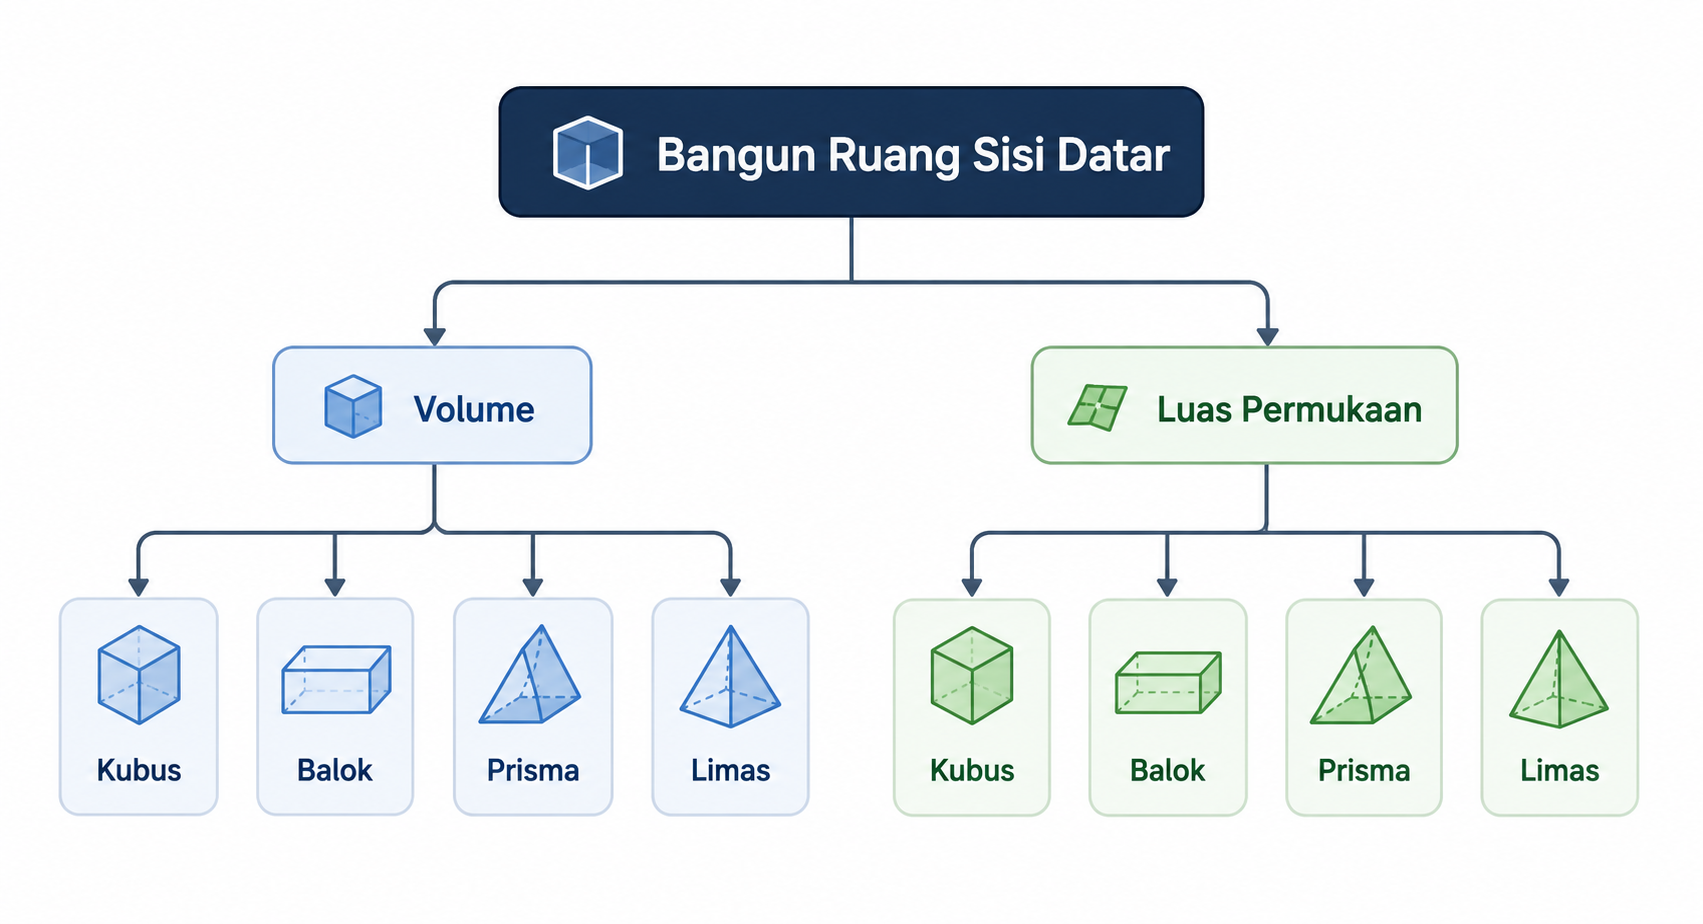
\includegraphics[width=0.8\textwidth]{images/bagan3.png}
            \caption{Struktur Hirarki Materi Bangun Ruang Sisi Datar}
            \label{fig:strukturmateri}
        \end{figure}
        Dari materi yang telah ditentukan, peneliti memilih beberapa materi yang dapat dijelaskan dengan simulasi 3D, yaitu:
        \begin{enumerate}[label=\arabic*.]
            \item Simulasi konsep volume pada kubus, menghitung banyaknya kubus satuan yang menyusun sebuah kubus.
            \item Simulasi konsep volume pada limas, sebuah kubus yang dapat berubah menjadi tiga buah limas dengan ukuran yang sama.
            \item Simulasi jaring-jaring bangun ruang kubus, balok, prisma, dan limas.
        \end{enumerate}
        \item Perancangan Media \\
        \hspace*{1cm}Peneliti merancang tampilan media dalam bentuk \textit{wireframe} sebagai panduan pengembangan antarmuka pengguna (\textit{UI}).
        \begin{figure}[H]
            \centering
            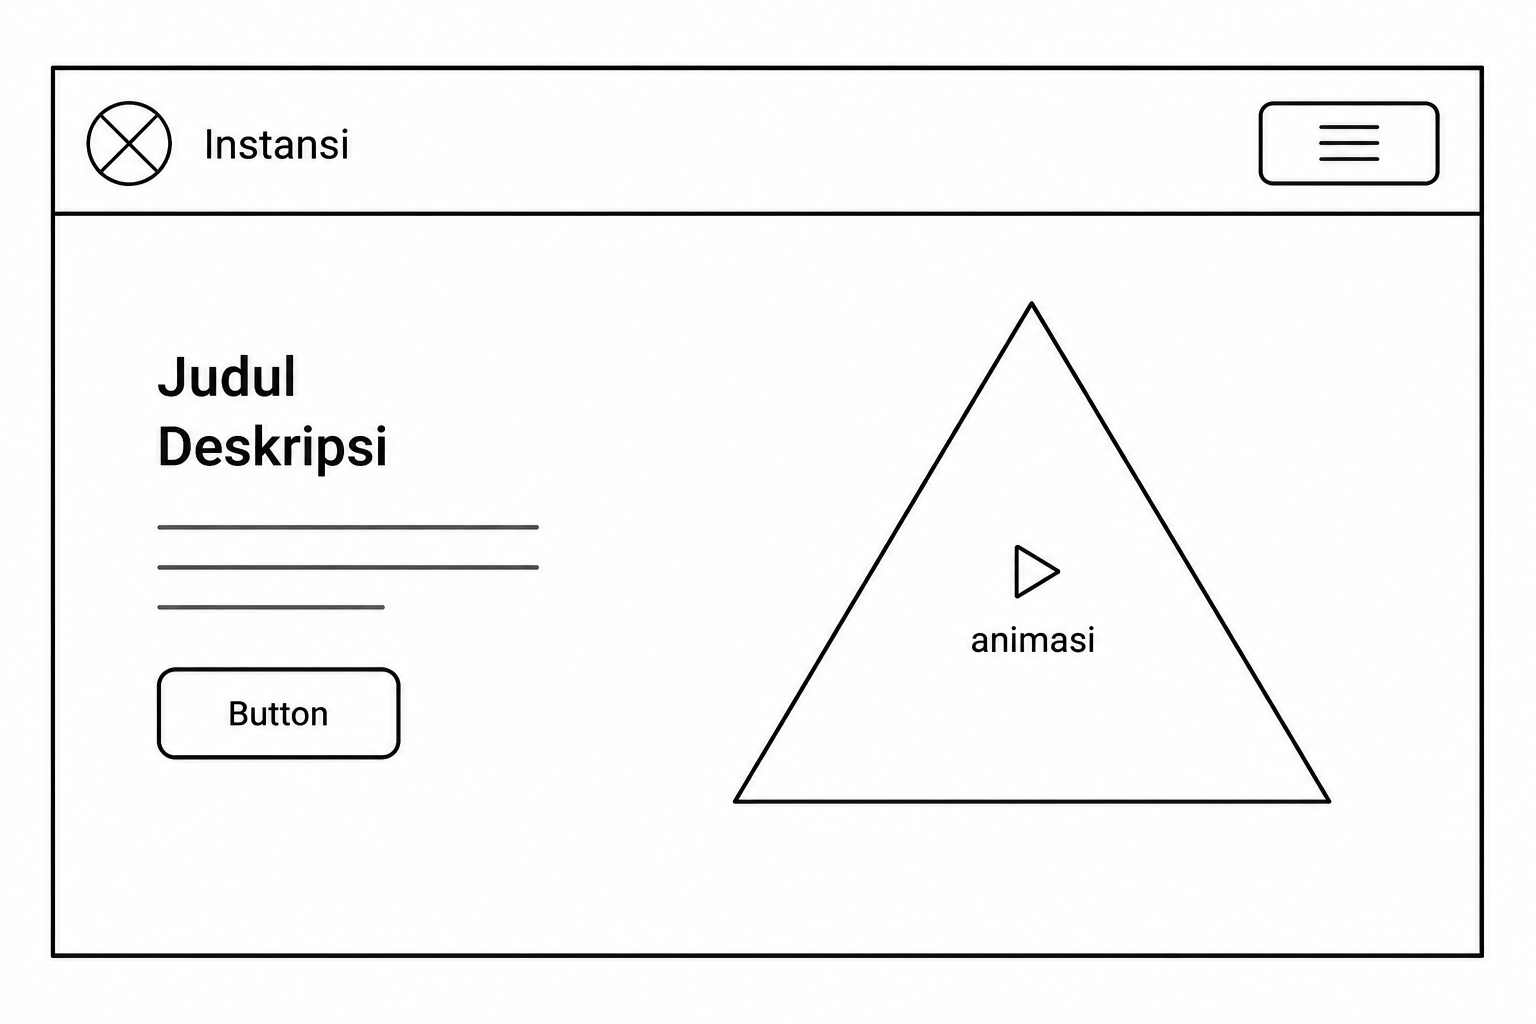
\includegraphics[width=0.8\textwidth]{images/landingpage3.png}
            \caption{\textit{Landing Page}}
            \label{fig:landingpage}
        \end{figure}
        \begin{figure}[H]
            \centering
            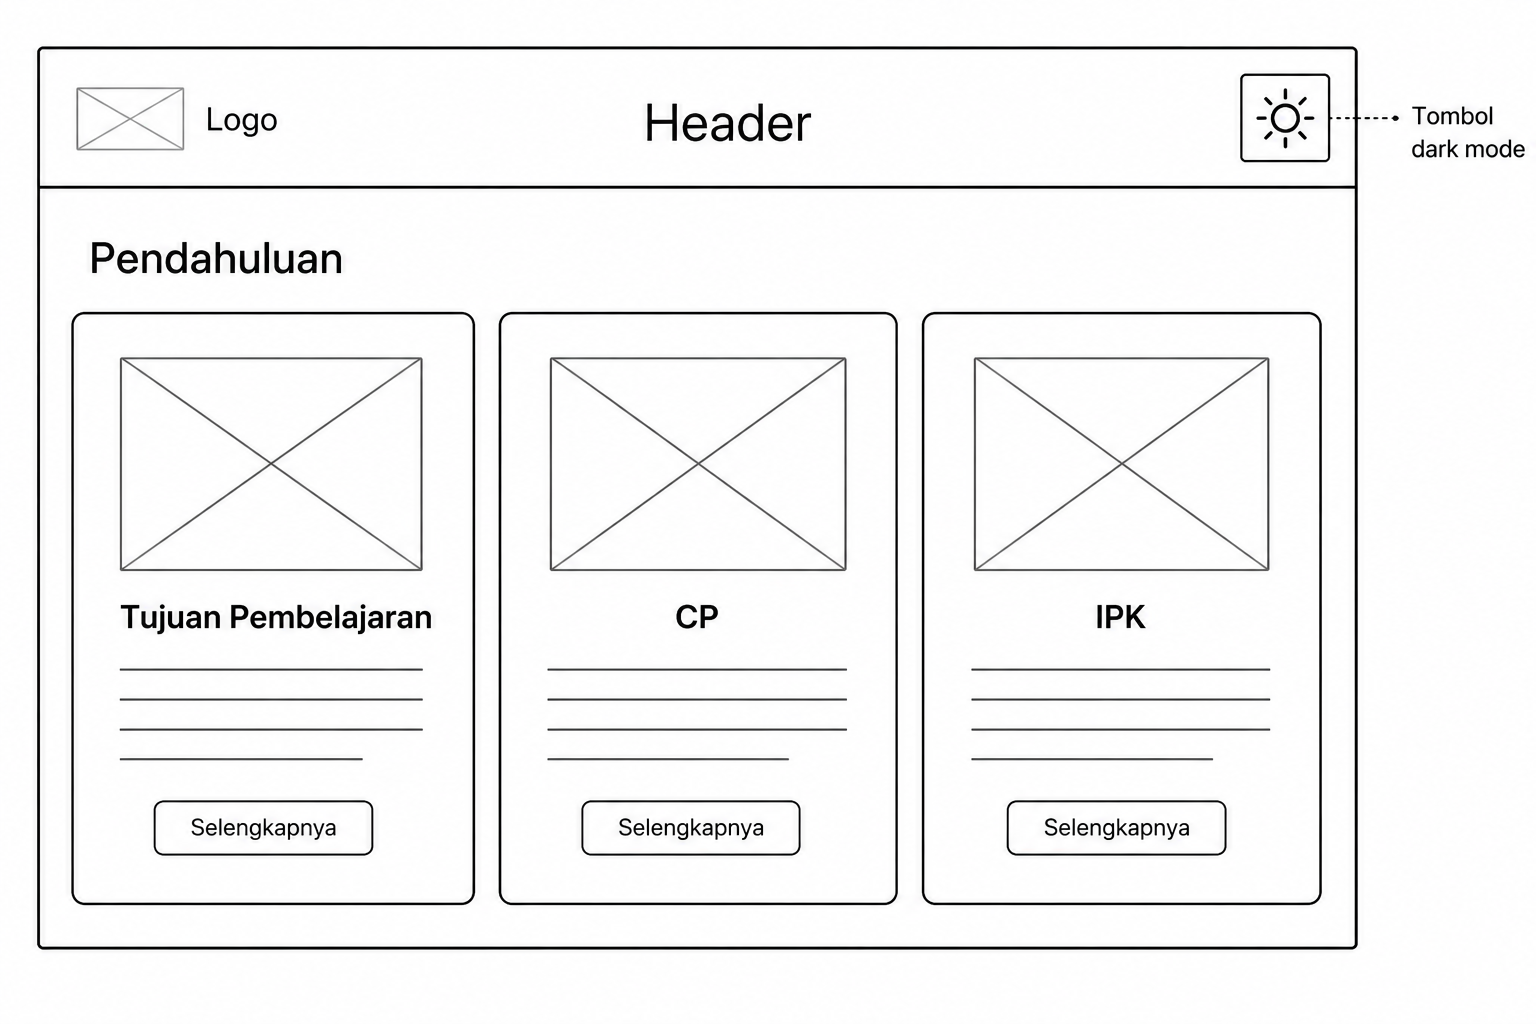
\includegraphics[width=0.8\textwidth]{images/pendahuluan3.png}
            \caption{Halaman Pendahuluan}
            \label{fig:pendahuluan}
        \end{figure}
        \begin{figure}[H]
            \centering
            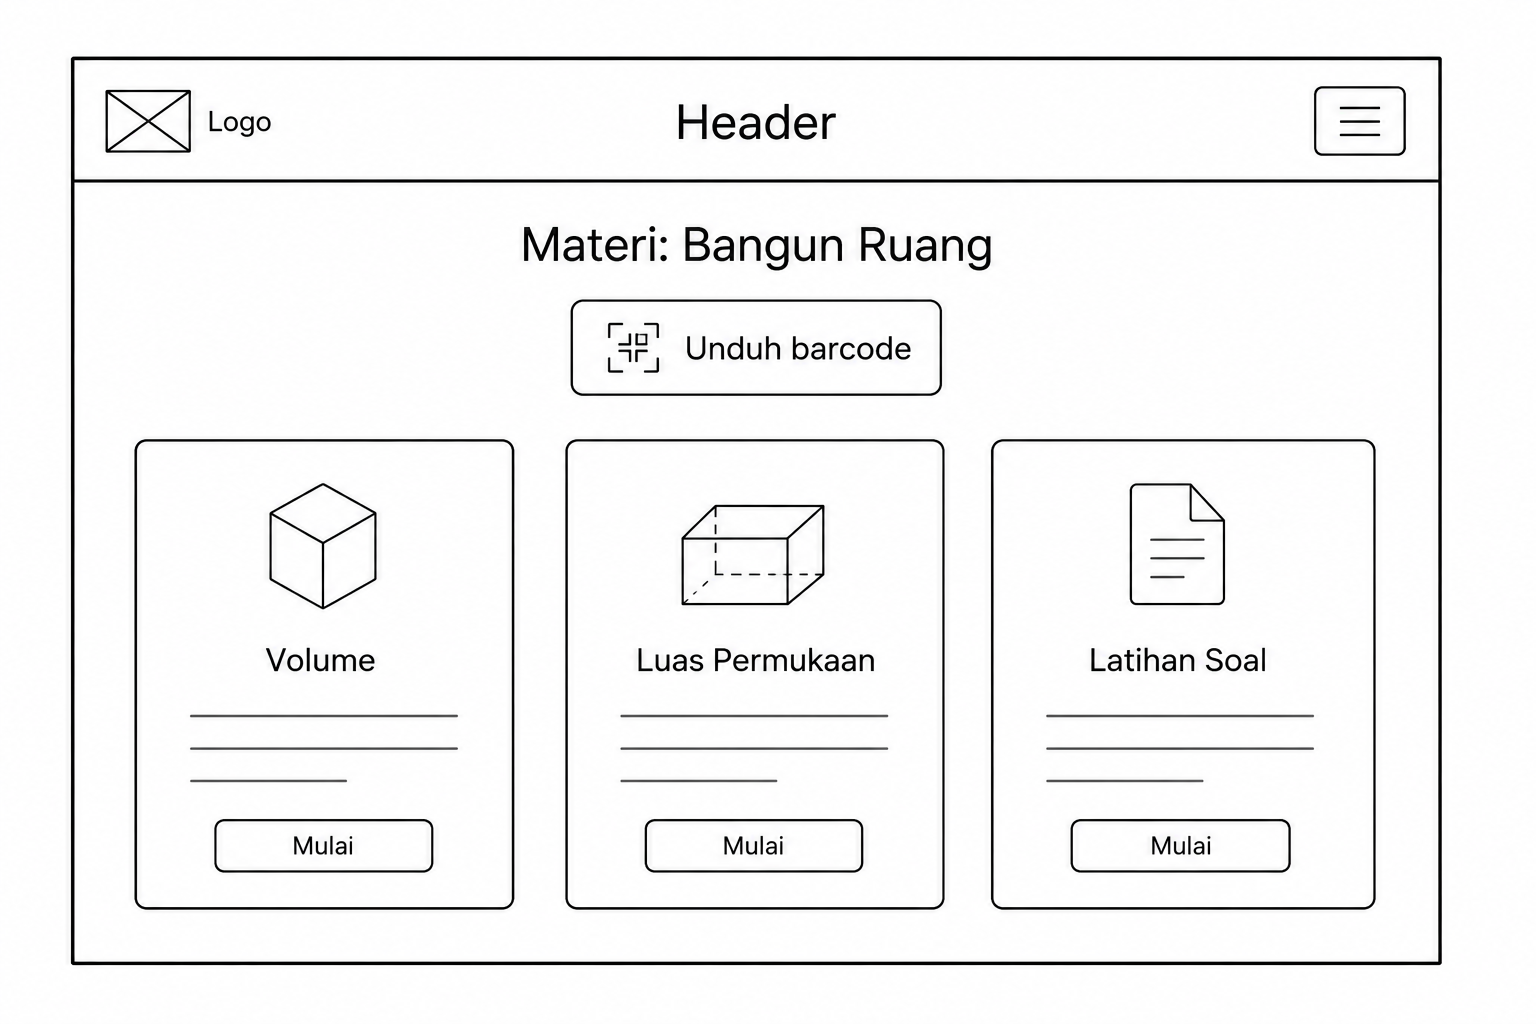
\includegraphics[width=0.8\textwidth]{images/menu3.png}
            \caption{Halaman Menu}
            \label{fig:halamanmenu}
        \end{figure}
        \begin{figure}[H]
            \centering
            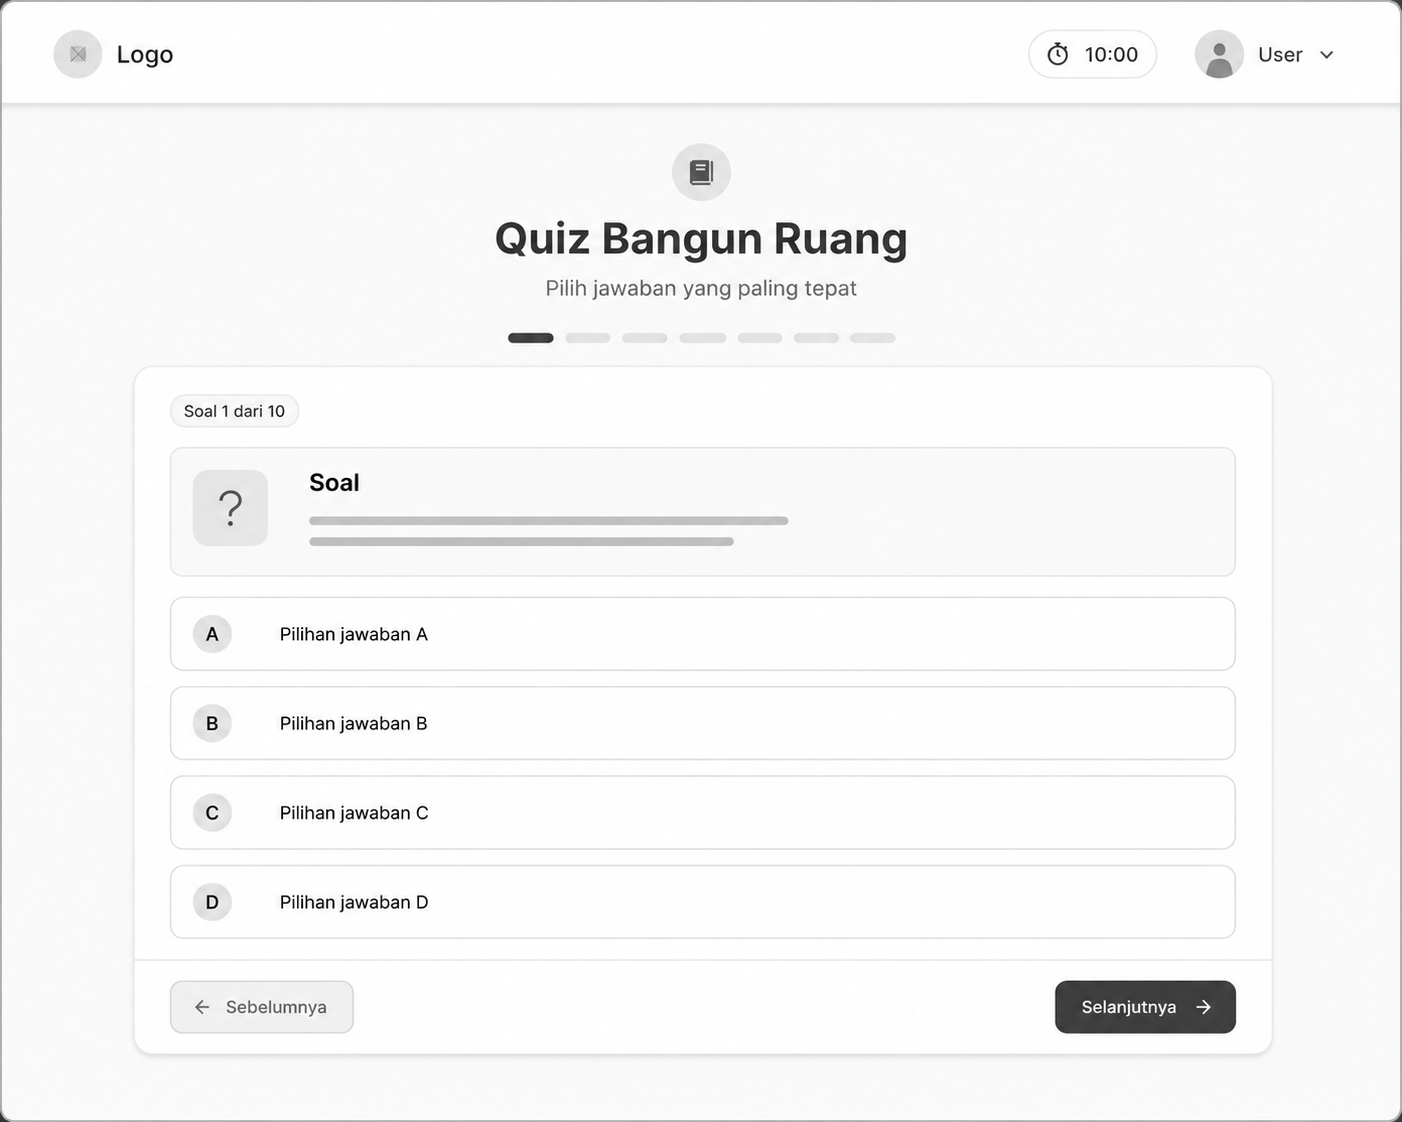
\includegraphics[width=0.8\textwidth]{images/quiz.png}
            \caption{Halaman Quiz}
            \label{fig:halamanquiz}
        \end{figure}
        Selain \textit{wireframe}, peneliti juga membuat diagram alur navigasi \textit{website} untuk mengilustrasikan struktur dan aliran interaksi pengguna.
        \begin{figure}[H]
            \centering
            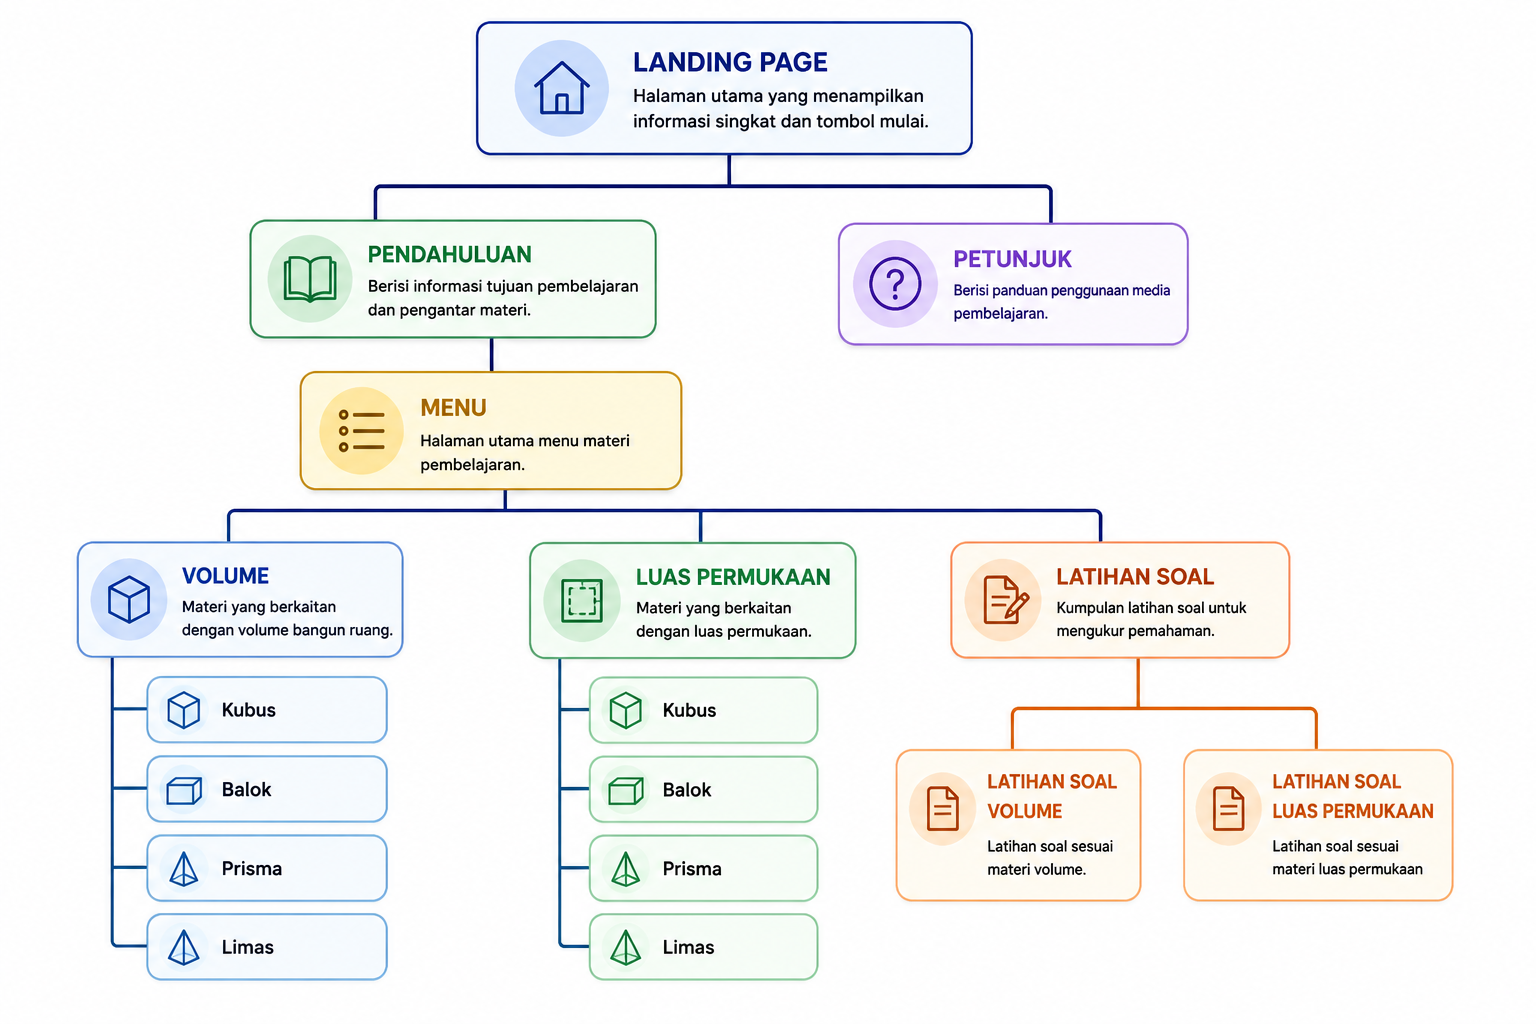
\includegraphics[width=0.8\textwidth]{images/flow2.png}
            \caption{Diagram Alur Navigasi Website}
            \label{fig:flowchart}
        \end{figure}
        \item Perancangan Interaksi Simulasi 3D
        \begin{figure}[H]
            \centering
            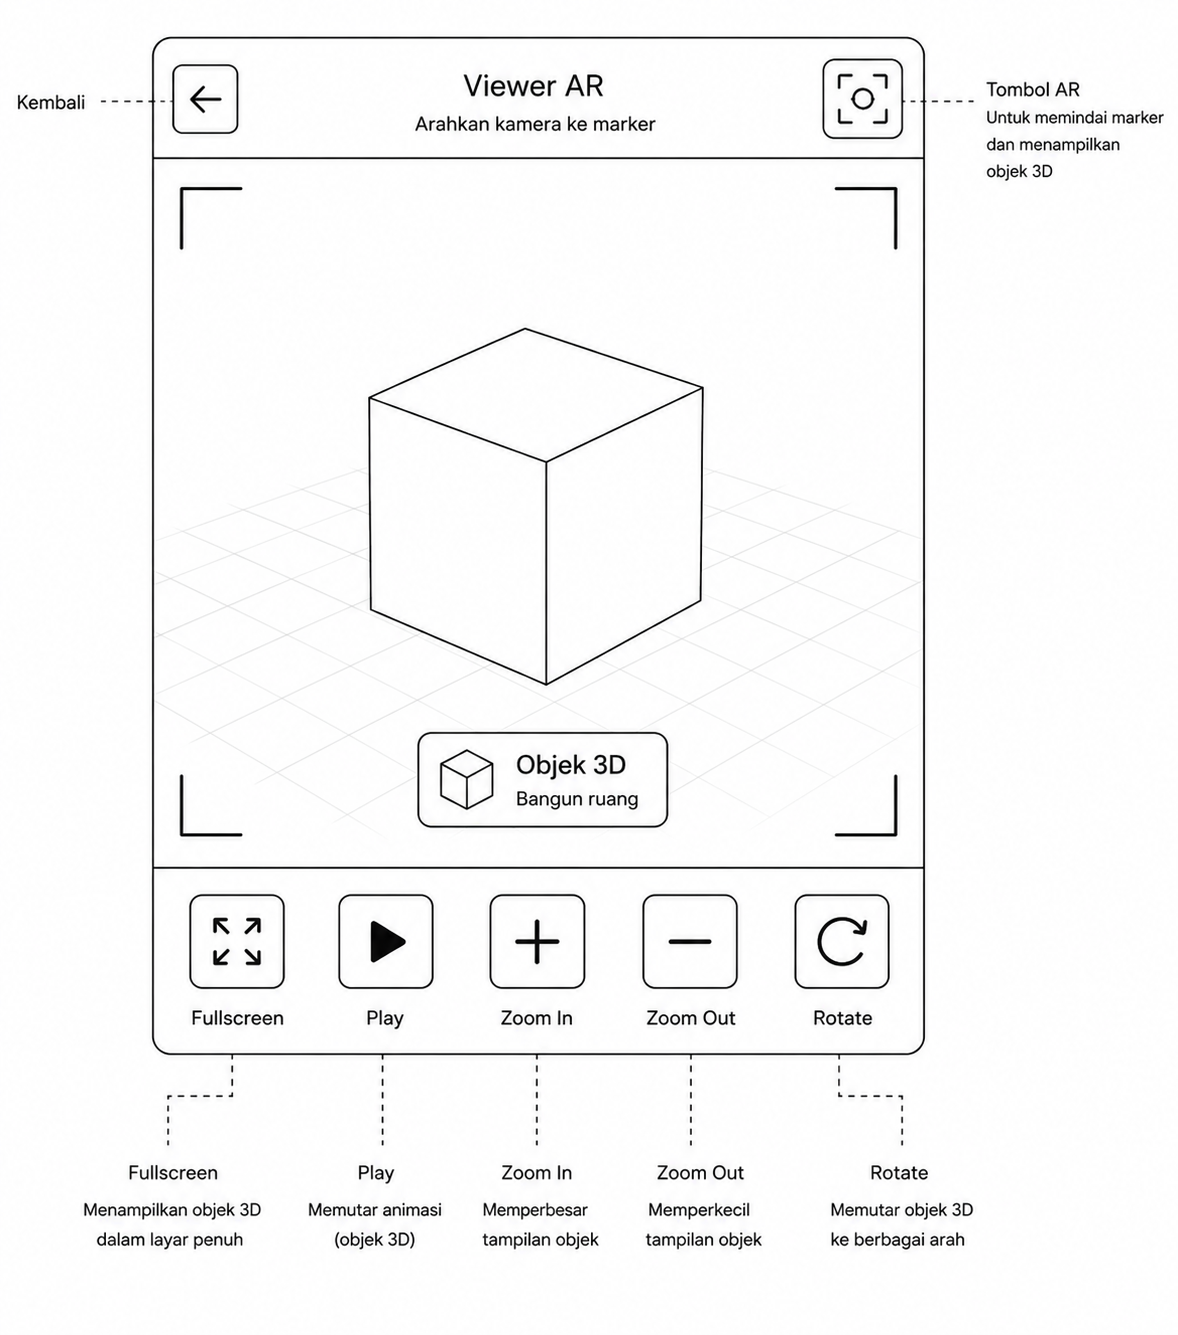
\includegraphics[width=0.5\textwidth]{images/wireframe3d.png}
            \caption{Halaman Simulasi 3D}
            \label{fig:mocksimulasi3d}
        \end{figure}
        \hspace*{1cm}Desain antarmuka halaman simulasi 3D ditampilkan pada Gambar \ref{fig:mocksimulasi3d}. Model 3D di tengah layar dapat dikendalikan melalui beberapa kontrol utama (Tabel \ref{tab:kontrolsimulasi3d}).
        \begin{table}[H]
            \centering
            \caption{Kontrol Utama Pada Halaman Simulasi 3D}
            \label{tab:kontrolsimulasi3d}
            \begin{tabular}{|p{3.5cm}|p{9cm}|}
                \hline
                \textbf{Kontrol} & \textbf{Fungsi} \\
                \hline
                Fullscreen & Berpindah ke tampilan layar penuh untuk memperbesar area visualisasi. \\
                \hline
                \textit{Play / Pause} & Menjalankan atau menghentikan animasi model 3D. \\
                \hline
                \textit{Zoom In / Zoom Out} & Memperbesar atau memperkecil tampilan objek. \\
                \hline
                \textit{Rotate} & Memutar objek dengan kecepatan konstan; dapat diaktifkan atau dinonaktifkan. \\
                \hline
                \textit{AR} & Berpindah ke mode \textit{Augmented Reality} (AR) dengan model 3D yang sama. \\
                \hline
            \end{tabular}
        \end{table}
        \item Perancangan Model 3D\\
        \hspace*{1cm}Model 3D dibuat menggunakan \textit{Blender}, meliputi kubus, balok, prisma, limas, serta jaring-jaring masing-masing bangun ruang. Semua model diekspor dalam format \texttt{.glb}.
        \item Perancangan Arsitektur Website\\
        \hspace*{1cm}Arsitektur \textit{website} dirancang sebagai aplikasi frontend berbasis \textit{React} (\textit{Single Page Application}). Pengembangan dilakukan secara lokal menggunakan \textit{Node.js} dan pengelola paket \textit{yarn}; seluruh kode sumber dikelola pada repositori \textit{GitHub}. Struktur penyimpanan dan alur data dirancang sebagai berikut:
        \begin{enumerate}[leftmargin=*, label=--]
            \item Aset statis (gambar, model 3D) disimpan pada Supabase Storage dan disajikan melalui URL publik.
            \item Komponen simulasi 3D diimplementasikan di sisi klien menggunakan \textit{Three.js} di dalam komponen \textit{React}.
            \item Integrasi \textit{AR} dilakukan melalui layanan eksternal mywebar.com; link atau QR code diintegrasikan ke dalam aplikasi \textit{React}.
            \item Variabel lingkungan sensitif disimpan sebagai secret pada pengaturan \textit{Vercel}.
            \item \textit{Continuous Deployment}: setiap perubahan pada cabang utama GitHub memicu build otomatis di \textit{Vercel} dan penerapan ke domain \textbf{https://medpemar.vercel.app}.
        \end{enumerate}
        \hspace*{1cm}Arsitektur ini memungkinkan pengembangan fitur tambahan di masa depan tanpa merombak keseluruhan sistem (Gambar \ref{fig:arsitekturweb}).
        \begin{figure}[H]
            \centering
            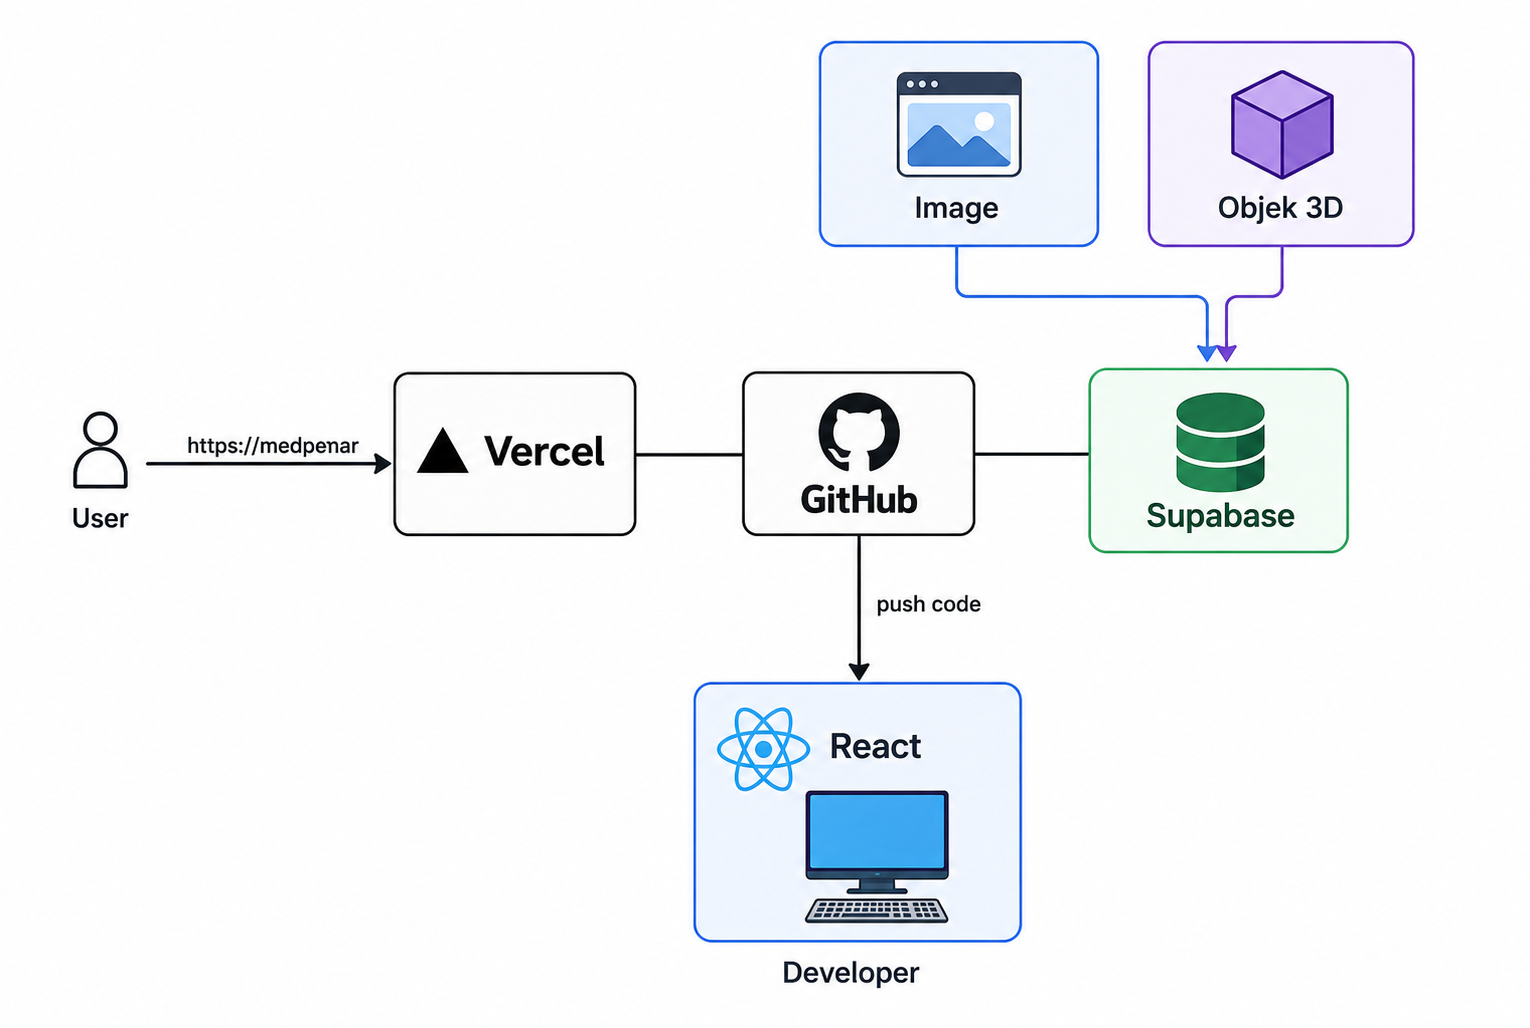
\includegraphics[width=0.9\textwidth]{images/Arsitektur.png}
            \caption{Arsitektur Website}
            \label{fig:arsitekturweb}
        \end{figure}
    \end{enumerate}

    \item \textbf{Pengembangan \textit{(Development)}}\\
    \hspace*{1cm}Pengembangan media pembelajaran berbasis simulasi 3D tergolong kompleks karena penggunaan \textit{React} dan \textit{Blender} dalam dunia pendidikan masih baru dengan referensi terbatas. Tahapan yang dilakukan meliputi implementasi desain, pengembangan antarmuka, pengembangan fitur simulasi 3D, pembuatan model 3D, pengembangan fitur evaluasi, integrasi sistem, validasi produk, dan revisi produk. Berikut penjabarannya.
    
    \begin{enumerate}[label=\arabic*)]
        \item Implementasi Desain\\
        \hspace*{1cm}Sesuai arsitektur pada Gambar \ref{fig:arsitekturweb}, implementasi dimulai dengan konfigurasi penyimpanan di Supabase dan pembuatan repositori di \textit{GitHub}. Selanjutnya, kode sumber di-\textit{clone} ke lingkungan lokal, diinstal dependensi (\textit{React} dan \textit{library} pendukung), kemudian dilakukan pengembangan antarmuka.
        \begin{enumerate}[leftmargin=*, label=--]
            \item Mengonfigurasi penyimpanan di Supabase untuk aset.
            \item Menyiapkan repositori \textit{GitHub}.
            \item Meng-\textit{clone} repositori ke lingkungan lokal.
            \item Menginstal dependensi, termasuk \textit{Three.js}.
            \item Memulai pengembangan antarmuka pengguna.
        \end{enumerate}
        \begin{figure}[H]
            \centering
            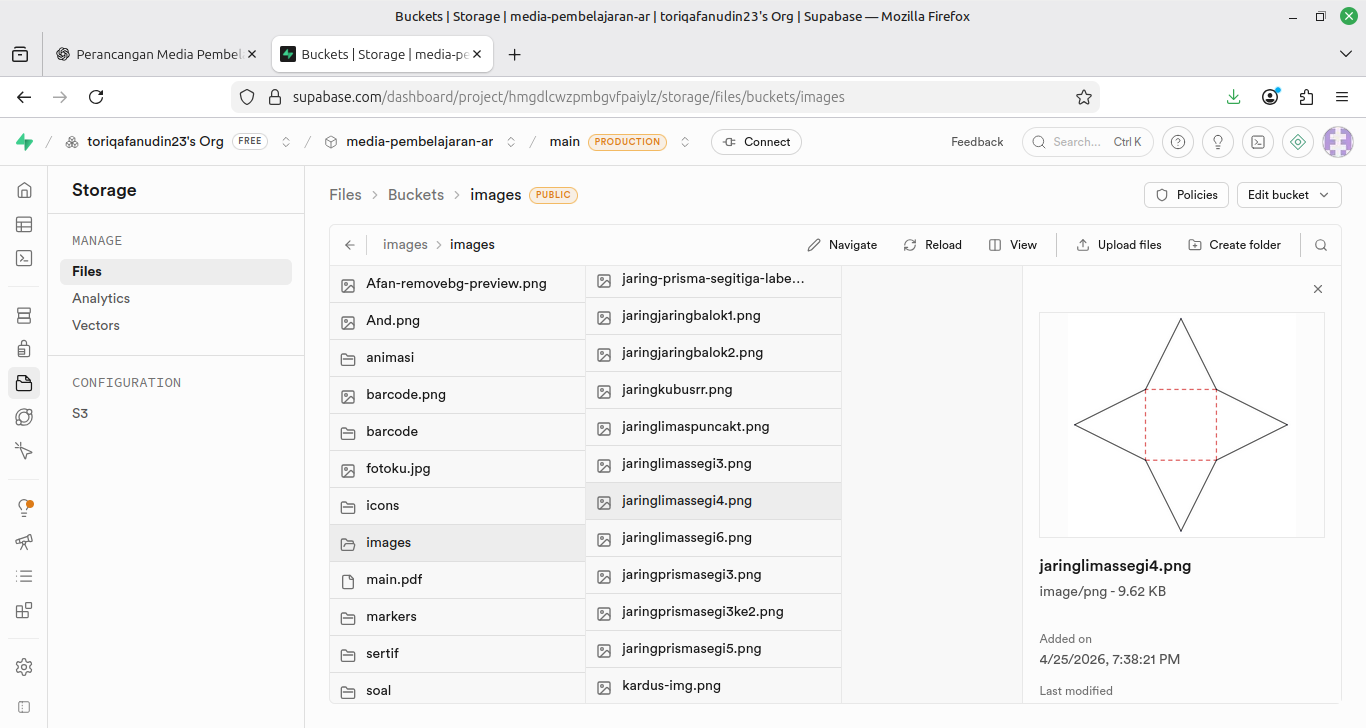
\includegraphics[width=1\textwidth]{images2/supabase.png}
            \caption{Storage di Supabase}
            \label{fig:supabase}
        \end{figure}
        \begin{figure}[H]
            \centering
            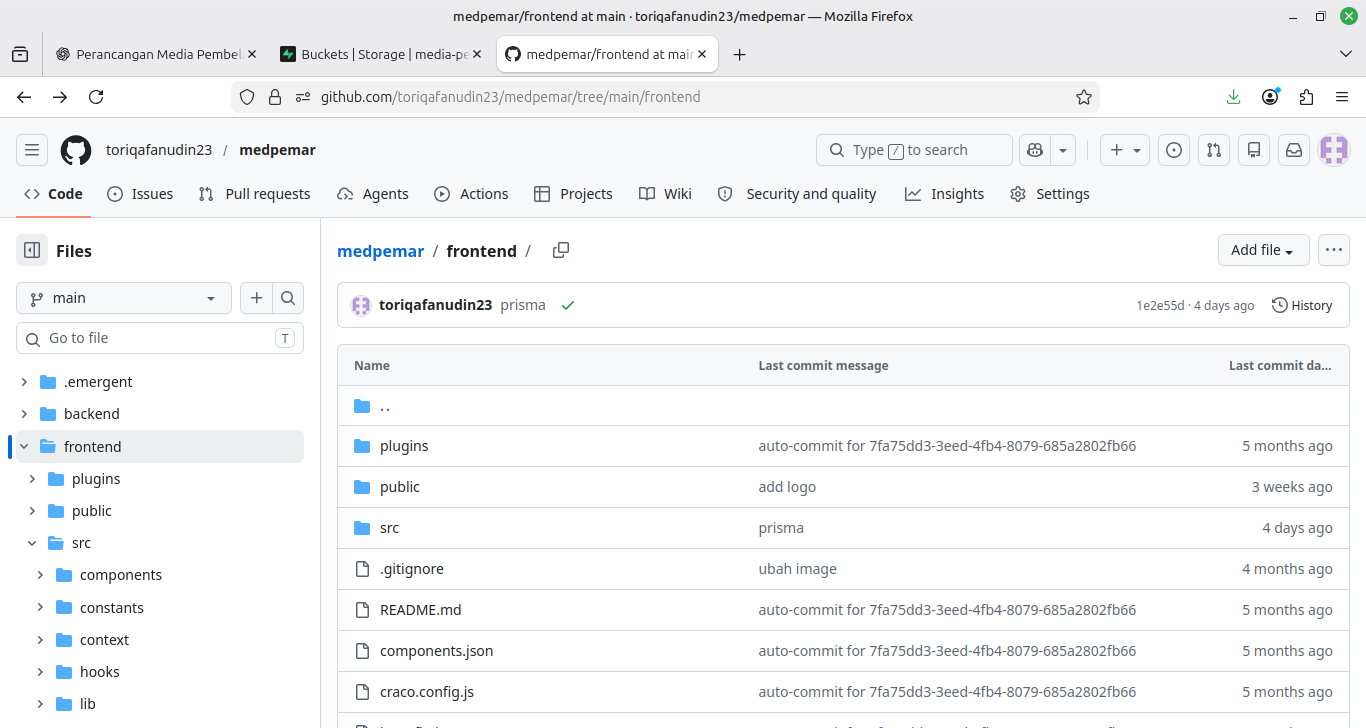
\includegraphics[width=1\textwidth]{images2/github.png}
            \caption{Repository di Github}
            \label{fig:github}
        \end{figure}
        \item Pengembangan Antarmuka\\
        \hspace*{1cm}Antarmuka dikembangkan menggunakan \textit{React} dan dirancang responsif. Peneliti mengintegrasikan \textit{Three.js} untuk menampilkan dan memanipulasi model 3D langsung di halaman \textit{website}. Berikut contoh hasil pengembangan antarmuka.
        \begin{figure}[H]
            \centering
            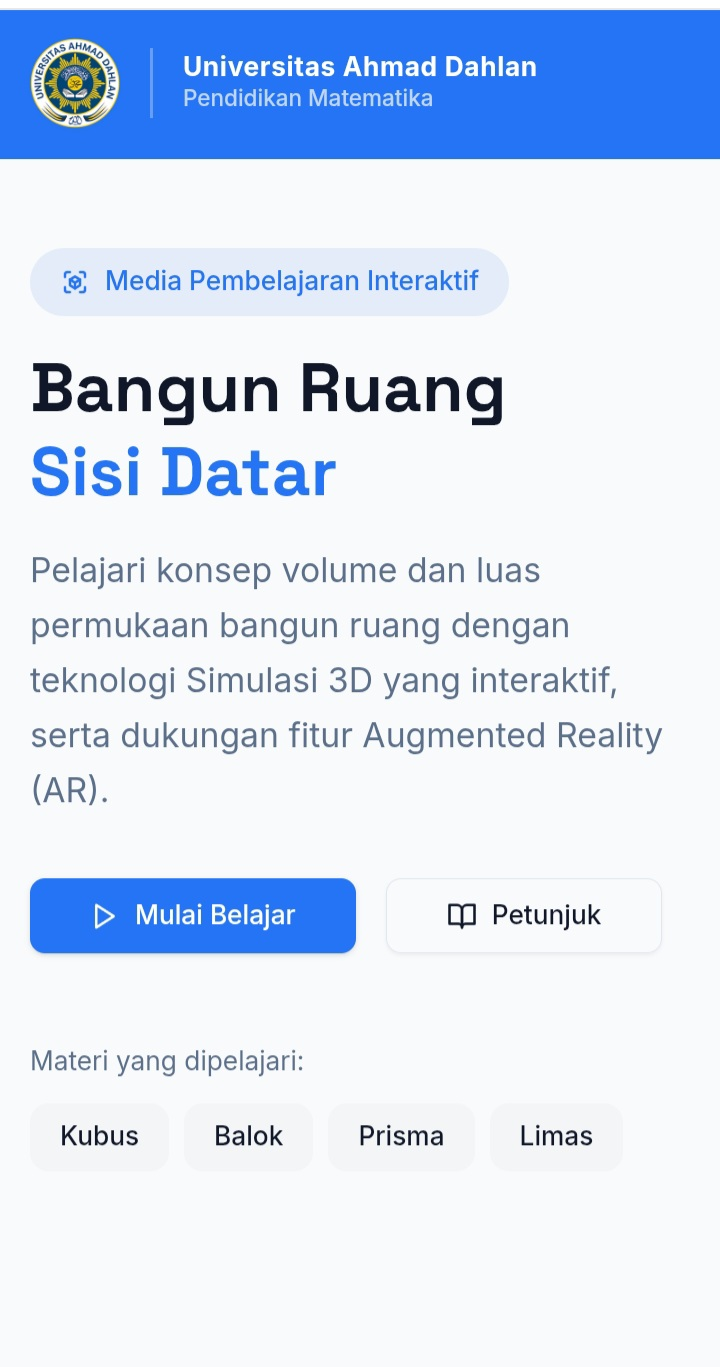
\includegraphics[width=0.3\textwidth]{images2/landingpage.jpg}
            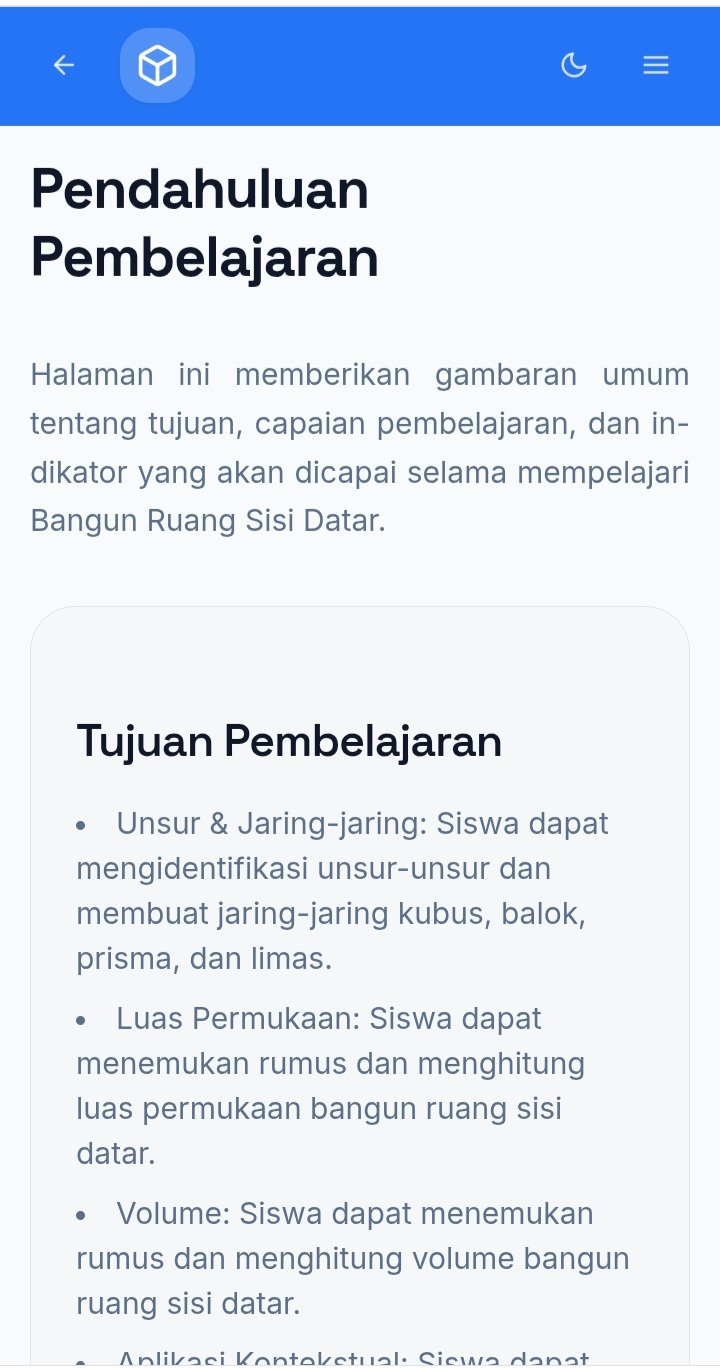
\includegraphics[width=0.3\textwidth]{images2/tujuanpembelajaran.jpg}
            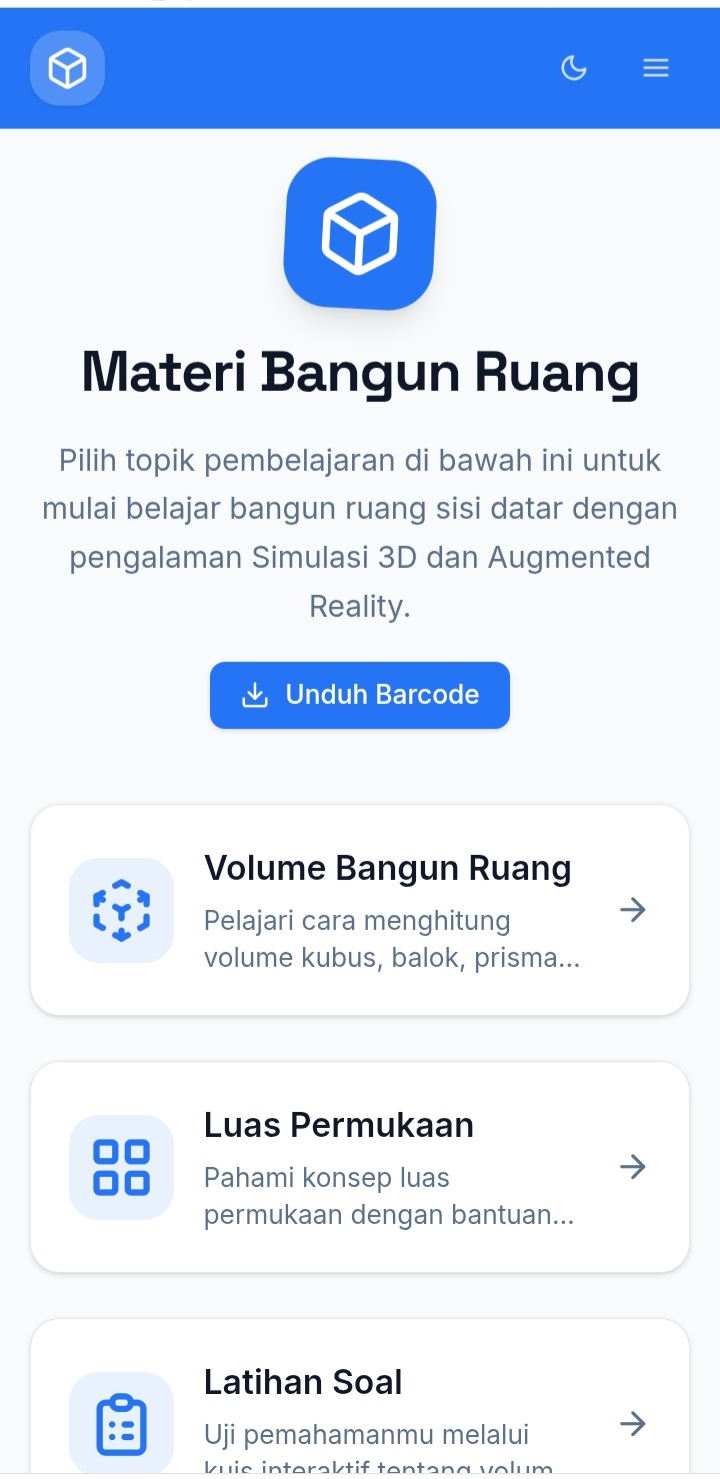
\includegraphics[width=0.3\textwidth]{images2/menu.jpg}
            \caption{Contoh Antarmuka Media Pembelajaran}
            \label{fig:antarmuka}
        \end{figure}

        \item Pembuatan Model 3D\\
        \hspace*{1cm}Pembuatan model 3D dilakukan menggunakan \textit{Blender} (perangkat lunak gratis dan \textit{open-source}). Peneliti membuat model kubus, balok, prisma, dan limas dengan geometri akurat serta animasi jaring-jaring. Semua model diekspor ke format \texttt{.glb} untuk kompatibilitas dengan \textit{Three.js}. Berikut tampilan \textit{Blender} dan contoh model yang dihasilkan.
        \begin{figure}[H]
            \centering
            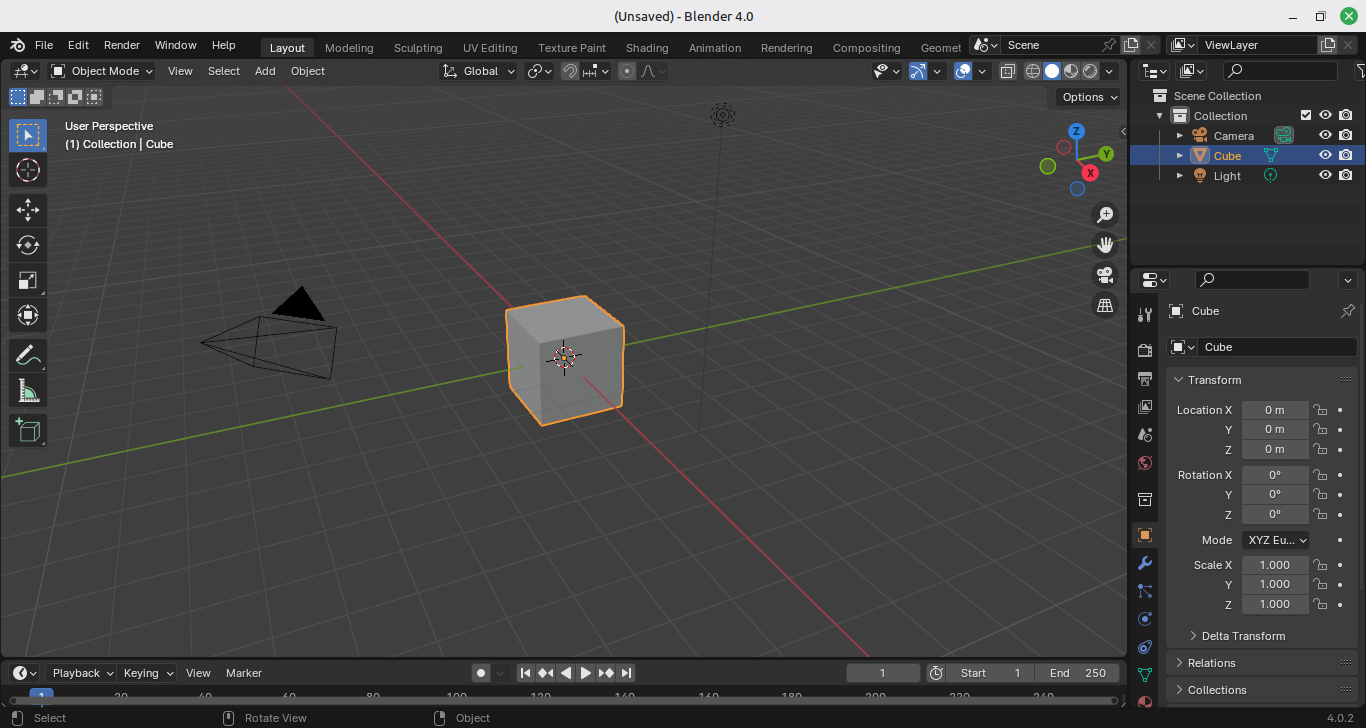
\includegraphics[width=1\textwidth]{images2/blender.png}
            \caption{Pembuatan Model 3D dengan \textit{Blender}}
            \label{fig:blender}
        \end{figure}
        \begin{figure}[H]
            \centering
            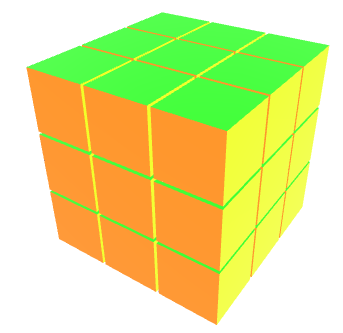
\includegraphics[width=0.3\textwidth]{images2/kubus.png}
            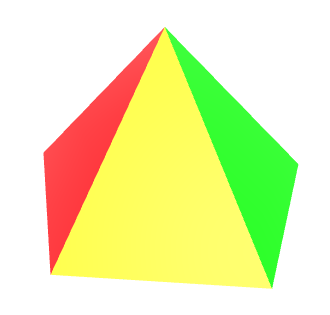
\includegraphics[width=0.3\textwidth]{images2/limas.png}
            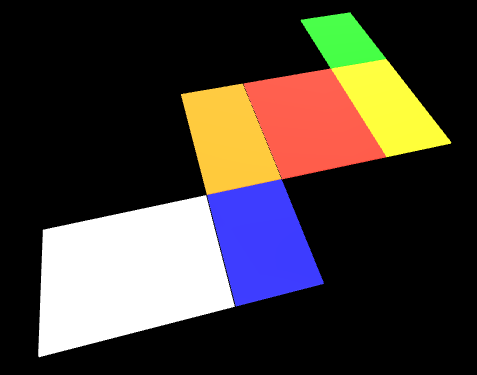
\includegraphics[width=0.3\textwidth]{images2/jaringbalok.png}
            \caption{Contoh Model 3D}
            \label{fig:contohobjek3d}
        \end{figure}
        
        \item Pengembangan Fitur Simulasi 3D\\
        \hspace*{1cm}Simulasi 3D diimplementasikan menggunakan \textit{Three.js} dalam komponen \textit{React}. Model 3D diupload ke Supabase Storage, kemudian komponen \textit{React} mengaksesnya untuk ditampilkan. Tombol kontrol sesuai Tabel \ref{tab:kontrolsimulasi3d}. Simulasi interaktif ini membantu peserta didik memahami konsep abstrak, antara lain:
        \begin{enumerate}[leftmargin=*, label=--]
            \item \textbf{Volume kubus:} Visualisasi kubus besar tersusun dari kubus satuan.
            \item \textbf{Volume limas:} Animasi transformasi kubus menjadi tiga limas sama ukuran.
            \item \textbf{Jaring-jaring:} Animasi pembukaan bangun ruang menjadi jaring-jaringnya.
        \end{enumerate}
        \begin{figure}[H]
            \centering
            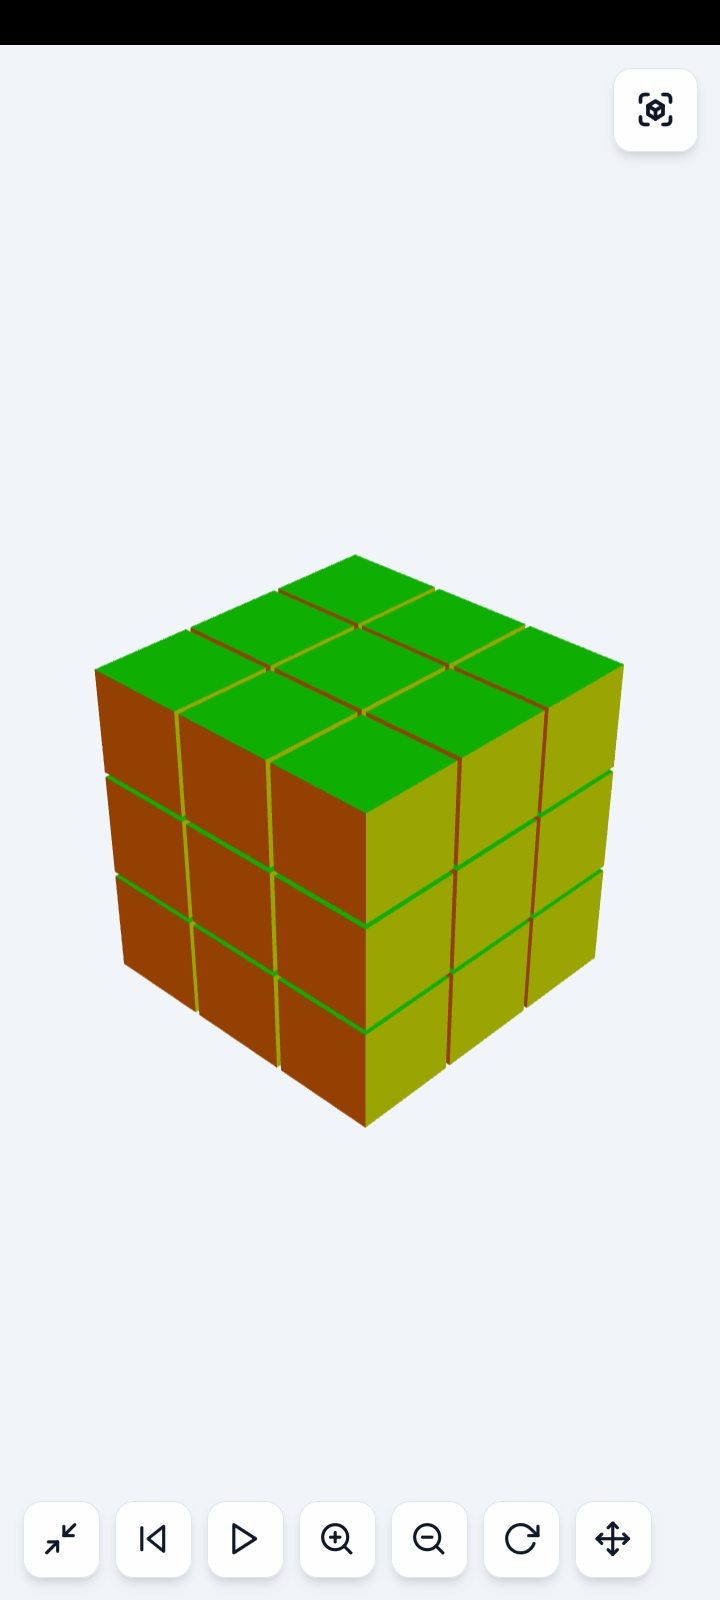
\includegraphics[width=0.35\textwidth]{images2/simulasi3d.jpg}
            \caption{Tampilan Simulasi 3D}
            \label{fig:simulasi3d}
        \end{figure}
        
        \item Menampilkan Model 3D melalui Fitur \textit{Augmented Reality} (\textit{AR})\\
        \hspace*{1cm}Peneliti mengintegrasikan fitur \textit{AR} menggunakan layanan MyWebAR untuk memperkaya pengalaman belajar. Keunggulan mywebar.com antara lain antarmuka intuitif, animasi model 3D tetap berfungsi dalam mode \textit{AR}, dan integrasi mudah dengan aplikasi \textit{website}. Proses pengembangan \textit{AR} meliputi upload model \texttt{.glb} ke mywebar.com, konfigurasi tampilan \textit{AR}, pembuatan link/QR code, dan integrasi ke komponen \textit{React}.
        \begin{figure}[H]
            \centering
            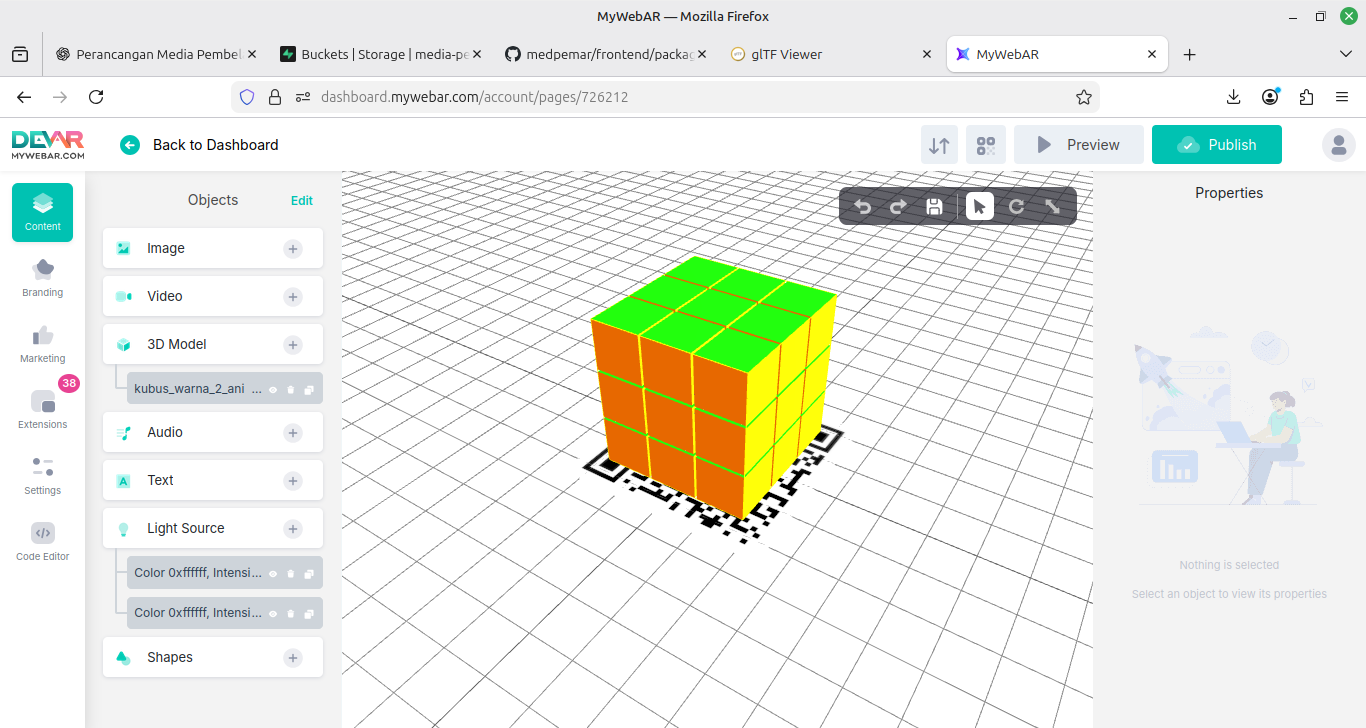
\includegraphics[width=1\textwidth]{images2/mywebar.png}
            \caption{Tampilan mywebar.com untuk Pengembangan \textit{AR}}
            \label{fig:mywebar}
        \end{figure}
        \begin{figure}[H]
            \centering
            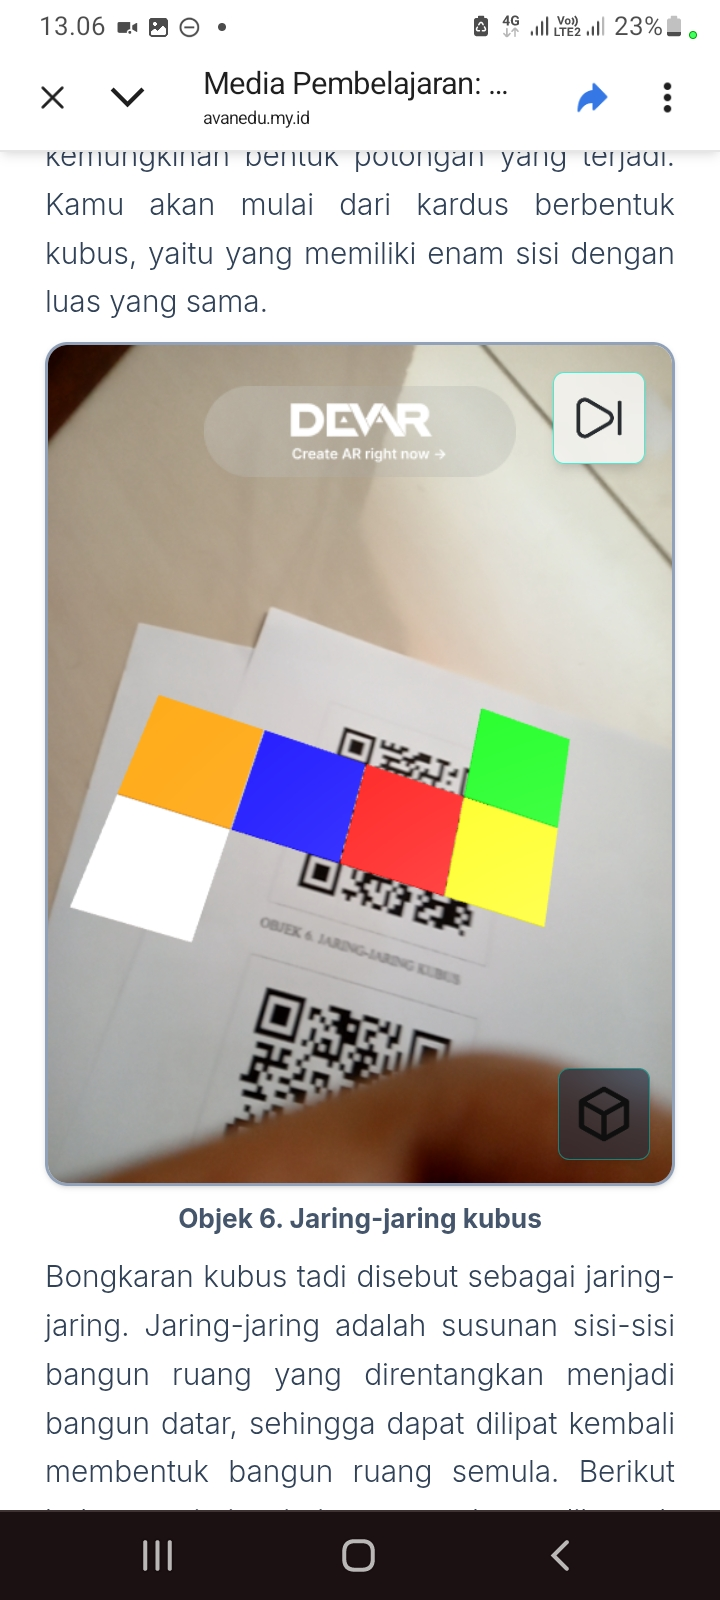
\includegraphics[width=0.3\textwidth]{images/materi4.jpg}
            \caption{Tampilan \textit{AR} pada Media Pembelajaran}
            \label{fig:armedia}
        \end{figure}
        
        \item Pengembangan Evaluasi\\
        \hspace*{1cm}Sistem evaluasi dirancang untuk memberikan umpan balik instan dan mendukung pembelajaran mandiri. Komponen evaluasi meliputi:
        \begin{enumerate}[leftmargin=*, label=--]
            \item \textbf{Isian singkat} selama pembelajaran sebagai \textit{checkpoint} pemahaman.
            \item \textbf{Soal evaluasi di akhir setiap bab} dengan pembahasan mendetail.
            \item \textbf{Fitur kuis interaktif} (Quiz Volume dan Quiz Luas Permukaan) dengan pembahasan setiap soal dan penilaian skor akhir.
        \end{enumerate}
        \begin{figure}[H]
            \centering
            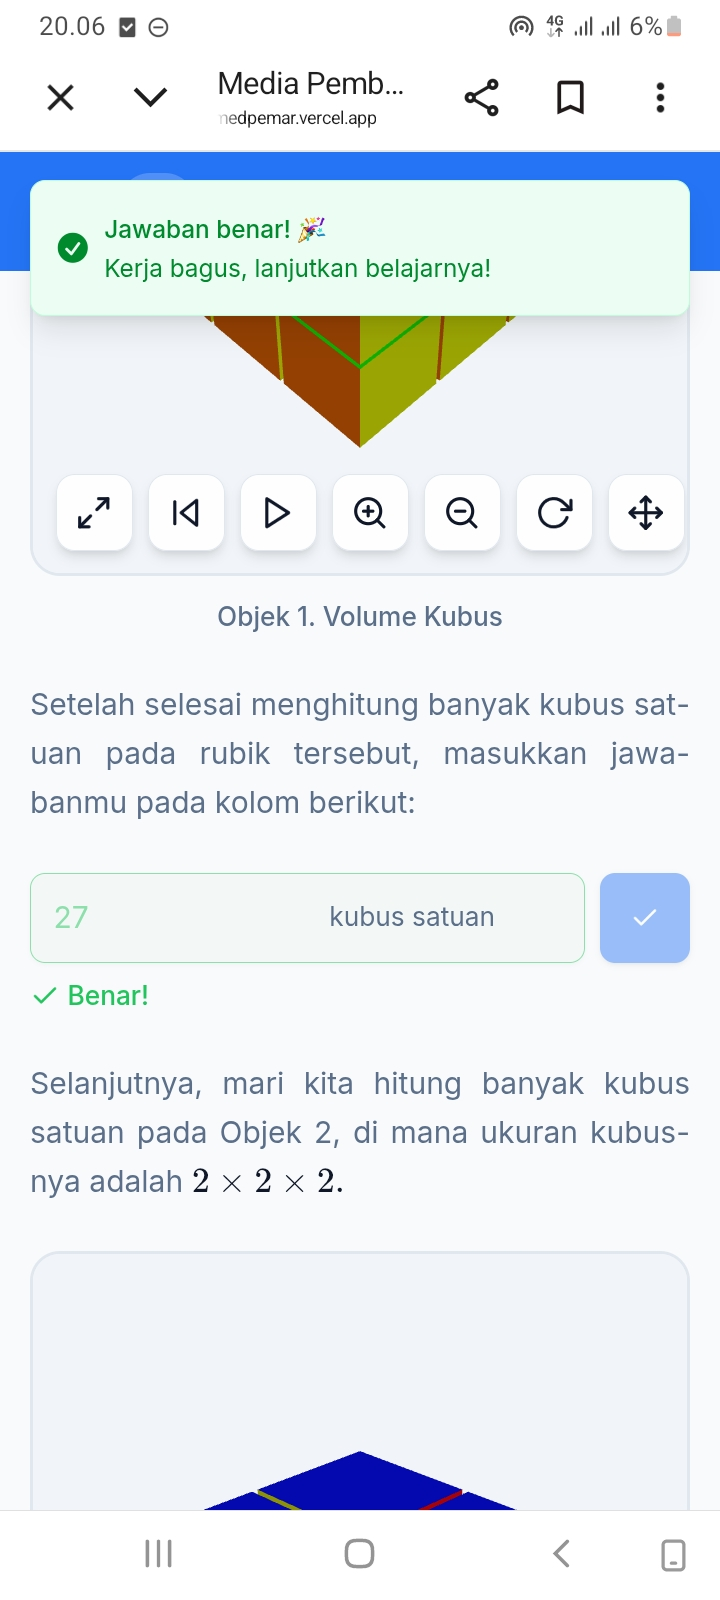
\includegraphics[width=0.3\textwidth]{images2/isiansingkat.jpg}
            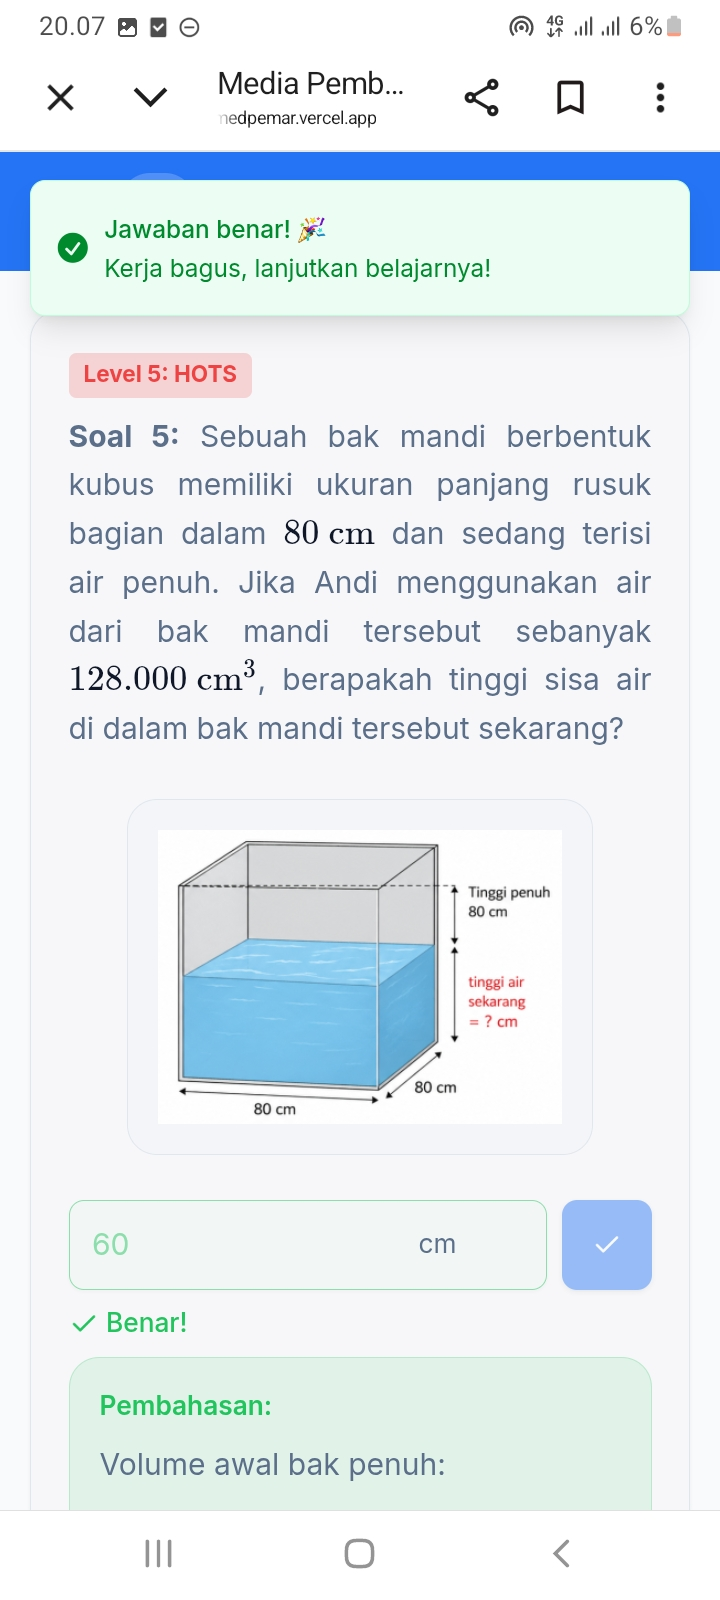
\includegraphics[width=0.3\textwidth]{images2/soalakhirbab.jpg}
            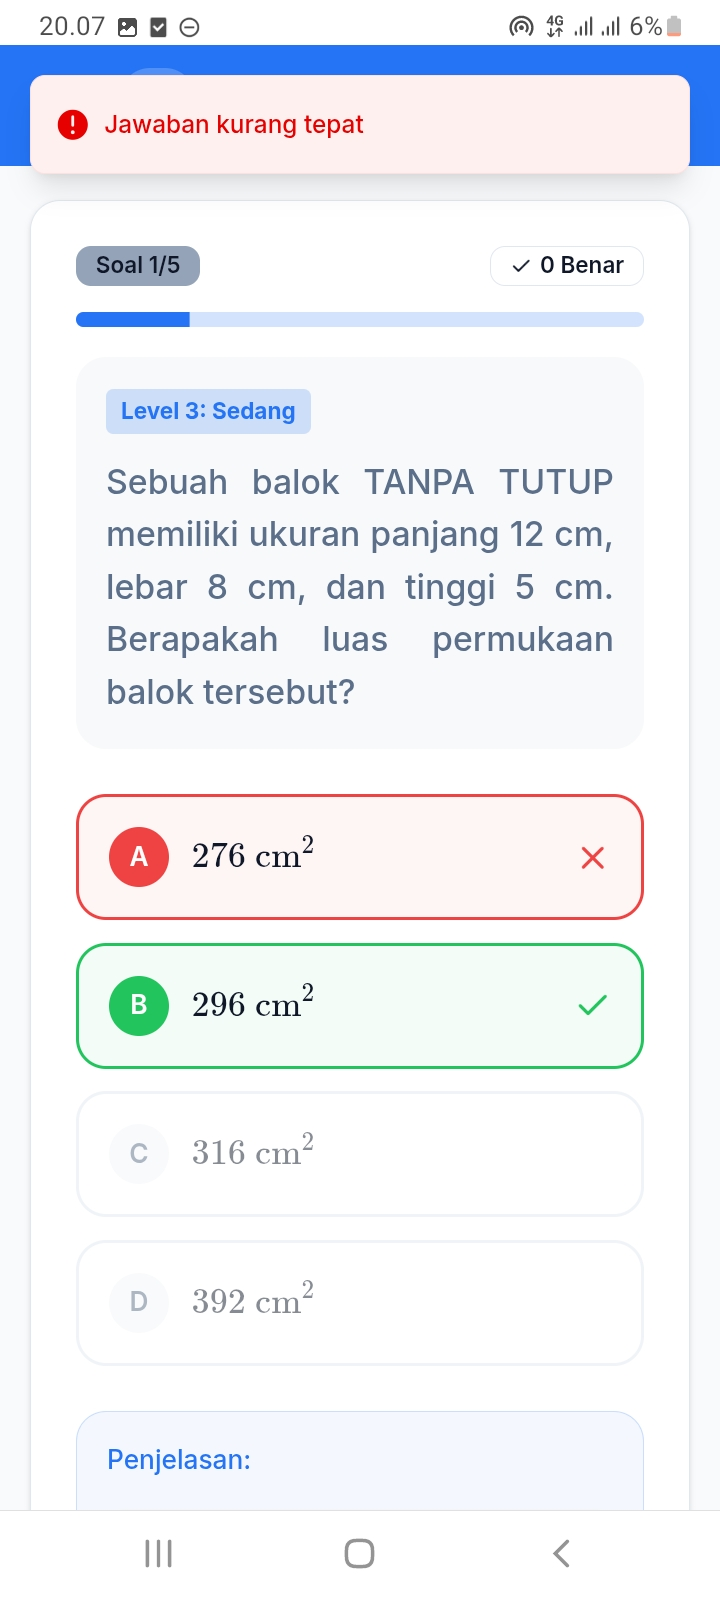
\includegraphics[width=0.3\textwidth]{images2/quizvolume.jpg}
            \caption{Contoh Soal Evaluasi}
            \label{fig:contohsoalevaluasi}
        \end{figure}
        \item Integrasi Sistem\\
        \hspace*{1cm}Semua komponen (model 3D dari \textit{Blender}, konten 2D, aset dari Supabase) diintegrasikan ke dalam aplikasi \textit{React}. Pengujian dilakukan untuk memastikan tidak ada eror dan performa optimal.

        \item Validasi Produk\\
        \hspace*{1cm}Validasi dilakukan oleh ahli materi dan ahli media untuk menilai kelayakan sebelum uji coba lapangan.
        
        \textbf{Validasi Ahli Materi:}
        
        \hspace*{1cm}Ahli materi terdiri atas:
        \begin{enumerate}[leftmargin=*, label=--]
            \item Ibu Rima Aksen Cahdriyana, M.Pd., dosen Pendidikan Matematika UAD.
            \item Bapak Wibowo Ramadhiyanto, S.Pd., pendidik Matematika SMP Muhammadiyah 9 Yogyakarta.
        \end{enumerate}
        
        \hspace*{1cm}Tujuan validasi adalah menilai keakuratan konten, kesesuaian dengan capaian pembelajaran, dan kelayakan materi untuk media simulasi 3D. Saran, masukan, dan tindak lanjut disajikan pada Tabel \ref{tabel:validasimateri}.
        \begin{table}[H]
\begin{adjustwidth}{-2cm}{-2cm}
    \centering
    \caption{Saran, Masukan, dan Tindak Lanjut Validasi Ahli Materi}
    \label{tabel:validasimateri}
    \begin{tabular}{|c|p{9cm}|c|}
        \hline
        \textbf{No} & \textbf{Saran dan Masukan} & \textbf{Tindak Lanjut} \\
        \hline
        1 & Perlu penambahan kata "satuan" pada kolom input kubus satuan. & Sudah direvisi \\
        \hline
        2 & Kalimat "kubus tersebut tidak terbentuk dari kubus satuan" kurang tepat secara konsep; diubah menjadi "tidak ditampilkan dalam bentuk kubus satuan". & Sudah direvisi \\
        \hline
        3 & Penggunaan istilah "representasi" kurang sesuai untuk siswa SMP; diganti dengan kalimat yang lebih sederhana. & Sudah direvisi \\
        \hline
        4 & Definisi prisma perlu diperbaiki. & Sudah direvisi \\
        \hline
        5 & Perlu penambahan paragraf pengantar sebelum definisi jaring-jaring. & Sudah direvisi \\
        \hline
        6 & Memperbanyak variasi jaring-jaring prisma. & Sudah direvisi \\
        \hline
        7 & Menambahkan Capaian Pembelajaran, Tujuan Pembelajaran, dan Indikator di awal \textit{website}. & Sudah direvisi \\
        \hline
    \end{tabular}
\end{adjustwidth}
\end{table}
\newpage
        
        \textbf{Validasi Ahli Media:}
        
        \hspace*{1cm}Ahli media terdiri atas:
        \begin{enumerate}[leftmargin=*, label=--]
            \item Bapak Anggit Prabowo, M.Pd., dosen Pendidikan Matematika UAD.
            \item Bapak Wibowo Ramadhiyanto, S.Pd., pendidik Matematika SMP Muhammadiyah 9 Yogyakarta.
        \end{enumerate}
        
        \hspace*{1cm}Tidak ada revisi signifikan; hanya kunci jawaban yang salah telah diperbaiki. Bapak Wibowo menyatakan bahwa media memiliki visual baik dan ilustrasi yang mempermudah pemahaman.
    \end{enumerate}

    \item \textbf{Implementasi}\\
    \hspace*{1cm}Uji coba produk dilakukan terhadap peserta didik kelas VIII-B dan VIII-D SMP Muhammadiyah 9 Yogyakarta untuk memperoleh informasi kelayakan. Uji coba terdiri atas dua jenis.
    \begin{enumerate}
        \item Uji Coba Kelas Kecil \\
        \hspace*{1cm}Dilaksanakan pada 18 Mei 2026 dengan 5 peserta didik kelas VIII-D yang dipilih secara acak. Peserta didik menggunakan media, kemudian mengisi angket. Hasil angket menunjukkan media memudahkan pemahaman, menarik, dan diharapkan dapat dikembangkan untuk materi lain. Tidak ada saran revisi.

        \item Uji Coba Kelas Besar \\
        \hspace*{1cm}Dilaksanakan pada 20 Mei 2026 dengan seluruh peserta didik kelas VIII-B (rekomendasi pendidik karena materi bangun ruang sedang diajarkan). Setelah pembelajaran, peserta didik mengisi angket. Mereka menyatakan materi mudah dipahami, pembelajaran tidak membosankan, namun menyarankan agar tidak terlalu banyak bacaan dan contoh soal diperbanyak.
    \end{enumerate}

    \item \textbf{Evaluasi}
    
    \hspace{1cm}Tahap evaluasi merupakan tahap akhir ADDIE untuk menganalisis hasil uji coba dan menyempurnakan produk sebelum menghasilkan produk akhir yang layak. Revisi akhir dilakukan berdasarkan masukan ahli materi, ahli media, dan peserta didik. Penilaian kelayakan mengacu pada kategori minimal "Baik".

\end{enumerate}

\textbf{B. Analisis Data}
\addcontentsline{toc}{section}{B. Analisis Data}

\hspace{1cm}Analisis data merupakan tahap lanjutan dari evaluasi. Data kualitatif dikonversi menjadi data kuantitatif. Media dinyatakan layak jika skor rata-rata minimal pada kategori "Baik". Berikut hasil analisis data:
\begin{enumerate}
    \item Analisis Penilaian Angket Ahli Materi\\
    \hspace*{1cm}Validasi materi dilakukan oleh dua ahli (Ibu Rima Aksen Cahdriyana, M.Pd. dan Bapak Wibowo Ramadhiyanto, S.Pd.). Hasil penilaian disajikan pada Tabel \ref{penilaianmateri}.
    \begin{table}[H]
        \begin{adjustwidth}{-2cm}{-2cm}
            \centering
            \caption{Hasil Penilaian Materi Pembelajaran Berdasarkan Aspek Penilaian}
            \label{penilaianmateri}
            \begin{tabular}{|l|c|c|c|l|}
                \hline
                \textbf{Aspek} & \textbf{Validator 1} & \textbf{Validator 2} & \textbf{Rata-rata Skor} & \textbf{Kategori Kualitatif}\\
                \hline
                Aspek Isi & \(4\) & \(4{,}71\) & \(4{,}35\) & Sangat Baik\\
                Aspek Bahasa & \(4\) & 5 & \(4{,}5\) & Sangat Baik\\
                Aspek Penyajian & \(4{,}5\) & \(4{,}87\) & \(4{,}68\) & Sangat Baik\\
                Aspek Simulasi 3D & \(5\) & 5 & 5 & Sangat Baik\\
                \hline
                \multicolumn{3}{|c|}{Kesimpulan} & \(4{,}63\) & Sangat Baik\\
                \hline
            \end{tabular}
        \end{adjustwidth}
    \end{table}

    \begin{table}[H]
        \centering
        \caption{Kriteria Penilaian Ahli Materi, Ahli Media, dan Respons Peserta Didik}
        \label{tab:kriteriaahli}
        \begin{tabular}{|c|c|l|}
            \hline
            \textbf{No} & \textbf{Rentang Skor \( (i) \) Kuantitatif} & \textbf{Kategori Kualitatif}\\
            \hline
            1 & \( \bar{x} > 4{,}2 \) & Sangat Baik\\
            2 & \( 3{,}4 < \bar{x} \leq 4{,}2 \) & Baik\\
            3 & \( 2{,}6 < \bar{x} \leq 3{,}4 \) & Cukup Baik\\
            4 & \( 1{,}8 < \bar{x} \leq 2{,}6 \) & Kurang\\
            5 & \( \bar{x} \leq 1{,8} \) & Sangat Kurang\\
            \hline 
        \end{tabular}
    \end{table}
    \hspace*{1cm}Rata-rata skor kedua validator adalah \(4{,}63\). Berdasarkan Tabel \ref{tab:kriteriaahli}, skor tersebut termasuk kategori \textbf{Sangat Baik}. Aspek simulasi 3D mendapat skor penuh (5) dari kedua validator.

    \item Analisis Penilaian Angket Ahli Media\\
    \hspace*{1cm}Validasi media dilakukan oleh dua ahli (Bapak Anggit Prabowo, M.Pd. dan Bapak Wibowo Ramadhiyanto, S.Pd.). Hasil penilaian disajikan pada Tabel~\ref{penilaianmedia}.
    \begin{table}[H]
        \begin{adjustwidth}{-2cm}{-2cm}
            \centering
            \caption{Hasil Penilaian Media Pembelajaran Berdasarkan Aspek Penilaian}
            \label{penilaianmedia}
            \begin{tabular}{|l|c|c|c|l|}
                \hline
                \textbf{Aspek} & \textbf{Validator 1} & \textbf{Validator 2} & \textbf{Rata-rata Skor} & \textbf{Kategori Kualitatif}\\
                \hline
                Kualitas Kegrafikan & \(4{,}33\) & \(4{,}91\) & \(4{,}62\) & Sangat Baik\\
                Kelayakan Bahasa & \(4{,}33\) & \(4{,}75\) & \(4{,}54\) & Sangat Baik\\
                Kualitas Perangkat Lunak & \(4{,}66\) & \(5\) & \(4{,}83\) & Sangat Baik\\
                \hline
                \multicolumn{3}{|c|}{Kesimpulan} & \(4{,}66\) & Sangat Baik\\
                \hline
            \end{tabular}
        \end{adjustwidth}
    \end{table}

    \hspace*{1cm}Rata-rata skor kedua validator adalah \(4{,}66\) (kategori \textbf{Sangat Baik}), dengan aspek kualitas perangkat lunak sangat baik (rata-rata \(4{,}83\)).

    \item Analisis Penilaian Angket Respons Peserta Didik\\
    \hspace*{1cm}Respons peserta didik diperoleh dari uji coba kelas kecil dan kelas besar. Kriteria penilaian mengacu pada Tabel \ref{tab:kriteriaahli}. Hasil uji coba kelas kecil disajikan pada Tabel~\ref{ujikelaskecil}.
    \begin{table}[H]
        \centering
        \caption{Data Hasil Ujicoba Kelas Kecil}
        \label{ujikelaskecil}
        \begin{tabular}{|c|l|c|l|}
            \hline
            \textbf{No} & \textbf{Nama} & \textbf{Rata-rata Skor} & \textbf{Kategori Kualitatif} \\
            \hline
            1 & Gilang Affan A. & \(4{,}35\) & Sangat Baik \\
            2 & Rachma Riski & \(4{,}85\) & Sangat Baik \\
            3 & Alif Bagas P. & \(4{,}15\) & Baik \\
            4 & Jasmine Sekar C. A. & \(3{,}38\) & Cukup Baik \\
            5 & Meydita Maharani & \(4{,}85\) & Sangat Baik \\
            \hline
            \multicolumn{2}{|c|}{Rata-rata Kelas Kecil} & \(4{,}31\) & Sangat Baik \\
            \hline
        \end{tabular}
    \end{table}
    Rata-rata kelas kecil \(4{,}31\) (kategori \textbf{Sangat Baik}). Peserta didik menyatakan media menarik dan mudah dipahami. Tidak ada revisi signifikan.
    
    \hspace*{1cm}Berdasarkan uji coba kelas besar (21 peserta didik kelas VIII-B), diperoleh hasil pada Tabel \ref{ujikelasbesar}.
    \begin{table}[H]
        \centering
        \caption{Data Hasil Ujicoba Kelas Besar}
        \label{ujikelasbesar}
        \begin{tabular}{|c|l|c|l|}
            \hline
            \textbf{No} & \textbf{Nama} & \textbf{Rata-rata Skor} & \textbf{Kategori Kualitatif} \\
            \hline
            1 & Athayya Anindya & \(4{,}96\) & Sangat Baik \\
            2 & Dimas Galih M. & \(4{,}62\) & Sangat Baik \\
            3 & Arletta Prada R. & \(4{,}96\) & Sangat Baik \\
            4 & Sinayang Kusuma N. & \(4{,}96\) & Sangat Baik \\
            5 & Zahra Nurlinda & \(4{,}88\) & Sangat Baik \\
            6 & Faiza Putri & \(4{,}92\) & Sangat Baik \\
            7 & Arawinda Putri A. & \(4{,}88\) & Sangat Baik \\
            8 & Kaffa Naura Kanifda & \(4{,}08\) & Baik \\
            9 & Daffa Raqillarafa & \(4{,}15\) & Baik \\
            10 & Tri Rui & \(4{,}35\) & Sangat Baik \\
            11 & Sandika Saputra & \(4{,}77\) & Sangat Baik \\
            12 & Chyntia Azzahra A. & \(5\) & Sangat Baik \\
            13 & Itsya Rama M. & \(4{,}62\) & Sangat Baik \\
            14 & Ilham & \(4{,}35\) & Sangat Baik \\
            15 & Adinda Kamelia & \(4{,}19\) & Baik \\
            16 & Rafa Abiyu S. & \(4{,}65\) & Sangat Baik \\
            17 & Callysta & \(4{,}96\) & Sangat Baik \\
            18 & Vaneza Aullisya L. & \(4{,}04\) & Baik \\
            19 & M. Isakhan Amir & \(4{,}58\) & Sangat Baik \\
            20 & Ibrahim Putra M. & \(5\) & Sangat Baik \\
            21 & Daffa Prakoso & \(4{,}73\) & Sangat Baik \\
            \hline
            \multicolumn{2}{|c|}{Rata-rata Kelas Besar} & \(4{,}65\) & Sangat Baik \\
            \hline
        \end{tabular}
    \end{table}
    Rata-rata kelas besar \(4{,}65\) (kategori \textbf{Sangat Baik}). Peserta didik memberikan respons positif, meskipun beberapa menyarankan penambahan jumlah contoh soal.

    \item Kualitas Produk Secara Keseluruhan\\
    \hspace*{1cm}Rata-rata keseluruhan dari ahli materi, ahli media, uji coba kelas kecil, dan uji coba kelas besar disajikan pada Tabel~\ref{ratakeseluruhan}.
    \begin{table}[H]
        \centering
        \caption{Hasil Rata-rata Keseluruhan}
        \label{ratakeseluruhan}
        \begin{tabular}{|c|l|c|l|}
            \hline
            \textbf{No} & \textbf{Sampel Uji Coba} & \textbf{Rata-rata} & \textbf{Kategori Kualitatif}\\
            \hline
            1 & Ahli Materi & \(4{,}63\) & Sangat Baik\\
            2 & Ahli Media & \( 4{,}66 \) & Sangat Baik\\
            3 & Uji Coba Kelas Kecil & \(4{,}31\) & Sangat Baik\\
            4 & Uji Coba Kelas Besar & \( 4{,}65 \) & Sangat Baik\\
            \hline
            \multicolumn{2}{|c|}{Rata-rata Keseluruhan} & \(4{,}56\) & Sangat Baik\\
            \hline
        \end{tabular}
    \end{table}
    \hspace*{1cm}Rata-rata keseluruhan \(4{,}56\) termasuk kategori \textbf{Sangat Baik}. Dengan demikian, media pembelajaran berbasis simulasi 3D dinyatakan layak digunakan untuk materi bangun ruang sisi datar kelas VIII.

\end{enumerate}

\newpage
\textbf{C. Revisi Produk}
\addcontentsline{toc}{section}{C. Revisi Produk}

\hspace*{1cm}Revisi produk dilakukan berdasarkan saran dan masukan dari ahli materi, ahli media, dan peserta didik.
\begin{enumerate}
    \item Revisi Produk Hasil Validasi Ahli Materi\\
    \hspace*{1cm}Perbaikan dilakukan sesuai saran ahli materi, meliputi:
    \begin{enumerate}
        \item Menambahkan kata "satuan" pada kolom input jawaban kubus satuan.
        \begin{table}[H]
            \centering
            \begin{tabular}{c c}
                Sebelum Revisi & Sesudah Revisi \\
                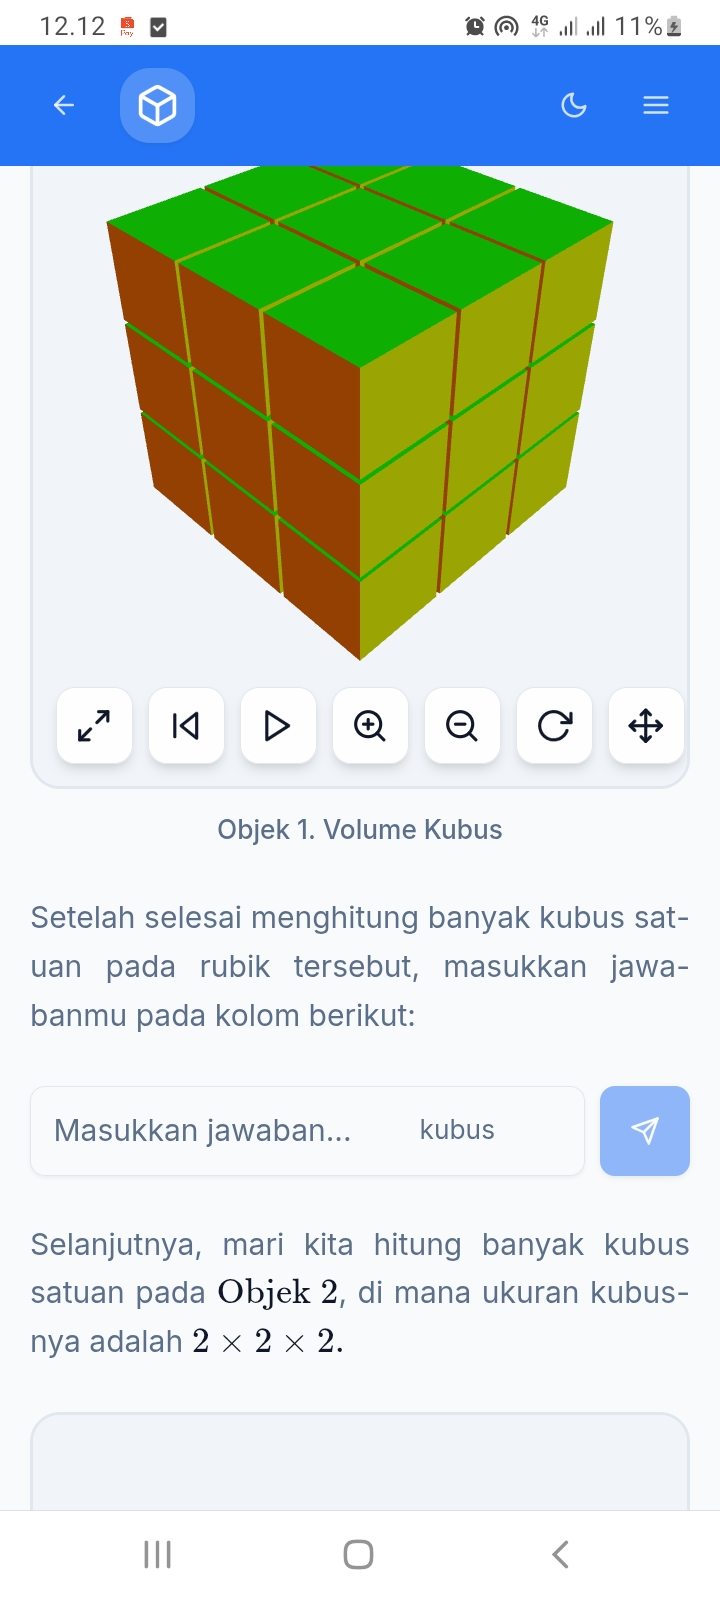
\includegraphics[width=0.25\textwidth]{revisi/sebelum/sebelumA.jpg} &
                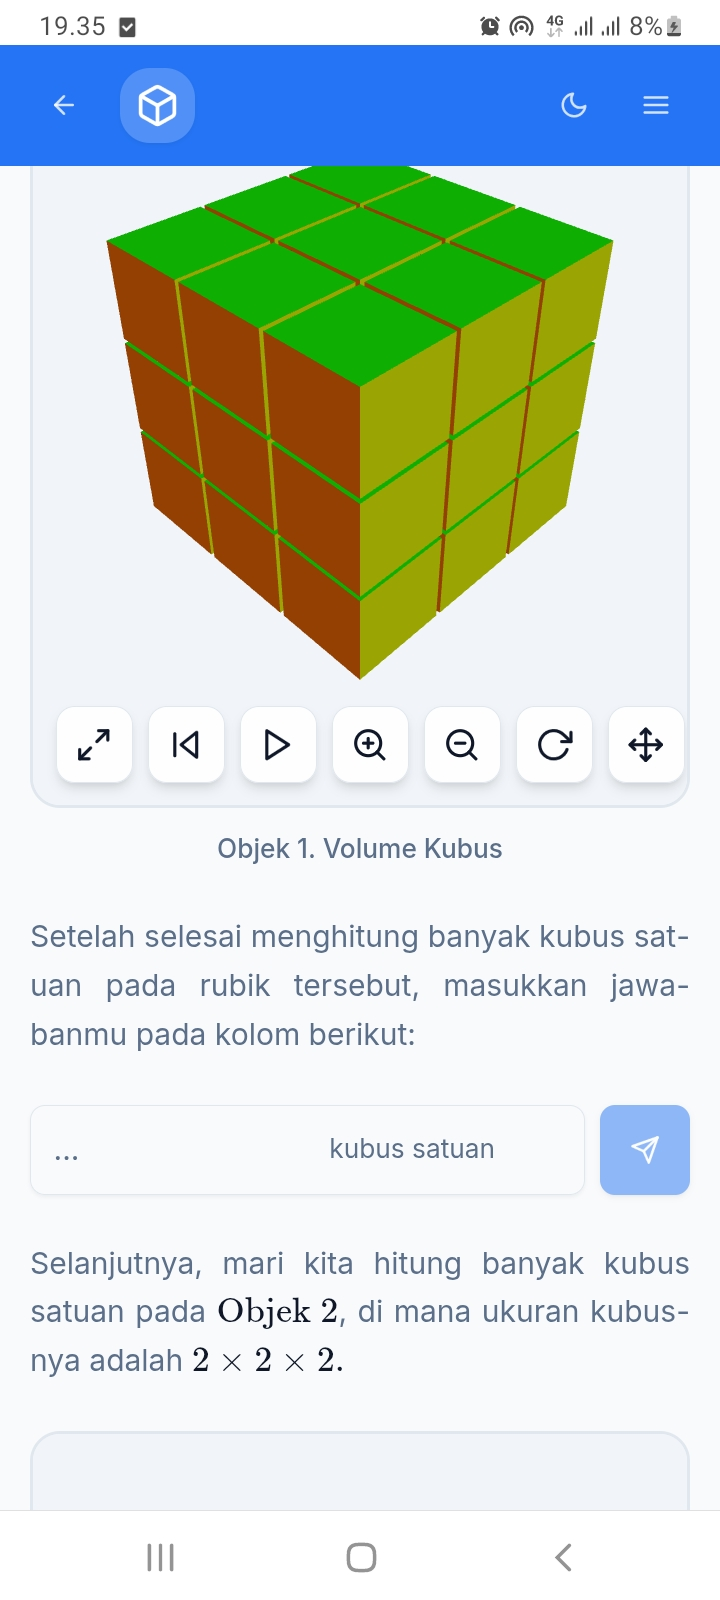
\includegraphics[width=0.25\textwidth]{revisi/sesudah/sesudahA.jpg} \\
            \end{tabular}
        \end{table}

        \item Memperbaiki definisi kubus yang kubus satuannya tidak ditampilkan.
        \begin{table}[H]
            \centering
            \begin{tabular}{c c}
                Sebelum Revisi & Sesudah Revisi \\
                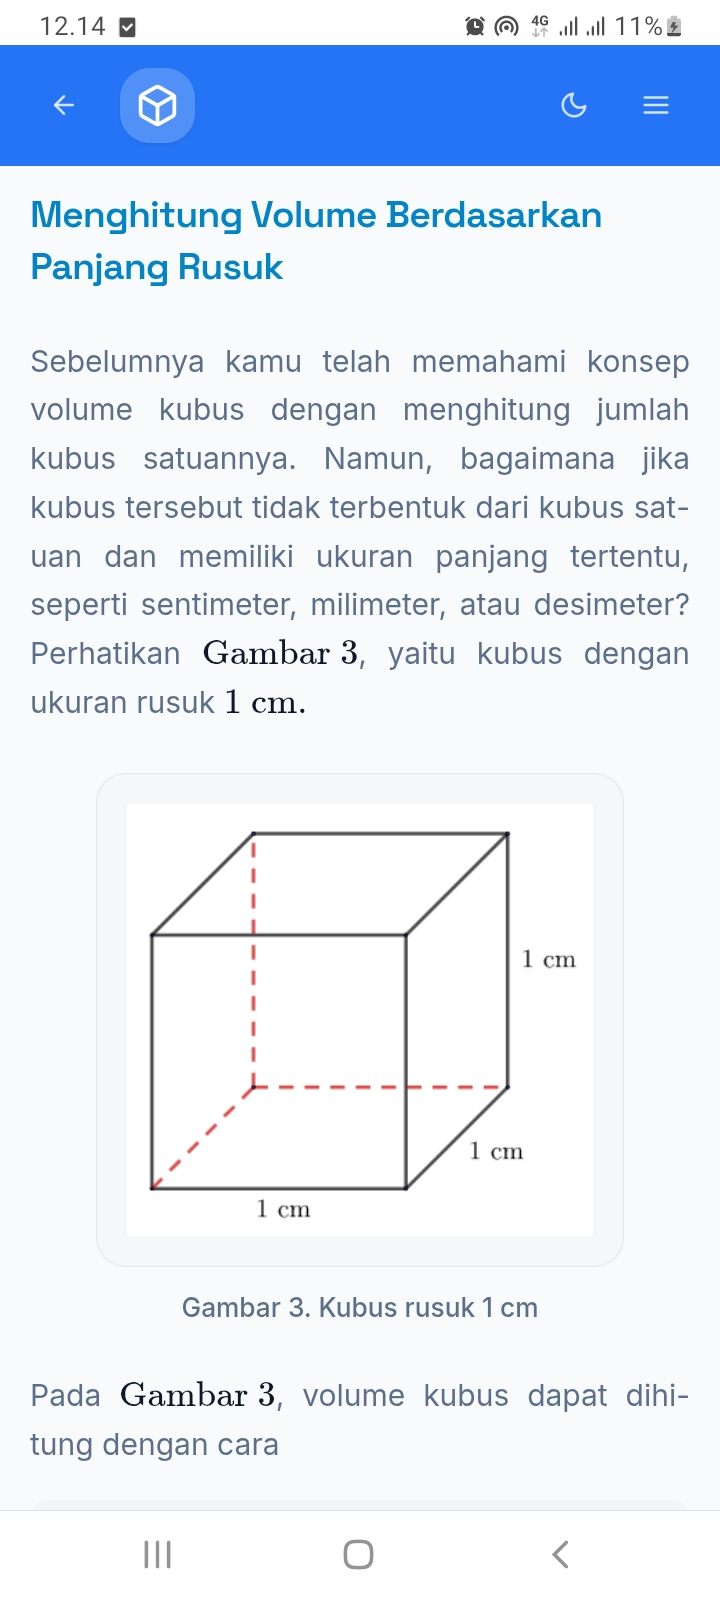
\includegraphics[width=0.25\textwidth]{revisi/sebelum/sebelumB.jpg} &
                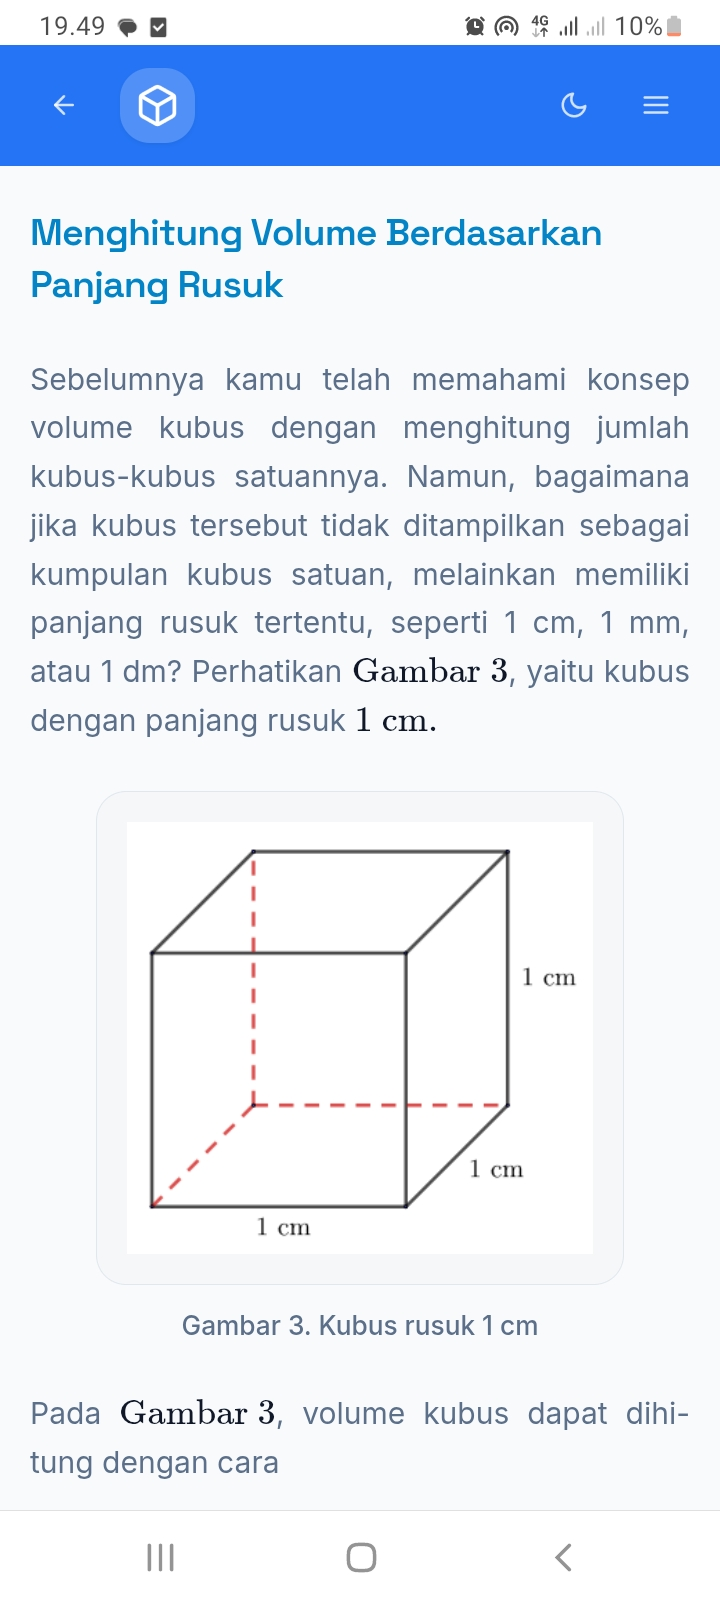
\includegraphics[width=0.25\textwidth]{revisi/sesudah/sesudahB.jpg} \\
            \end{tabular}
        \end{table}
        \item Mengganti kata "representasi" dengan kalimat yang lebih mudah dipahami.
        \begin{table}[H]
            \centering
            \begin{tabular}{c c}
                Sebelum Revisi & Sesudah Revisi \\
                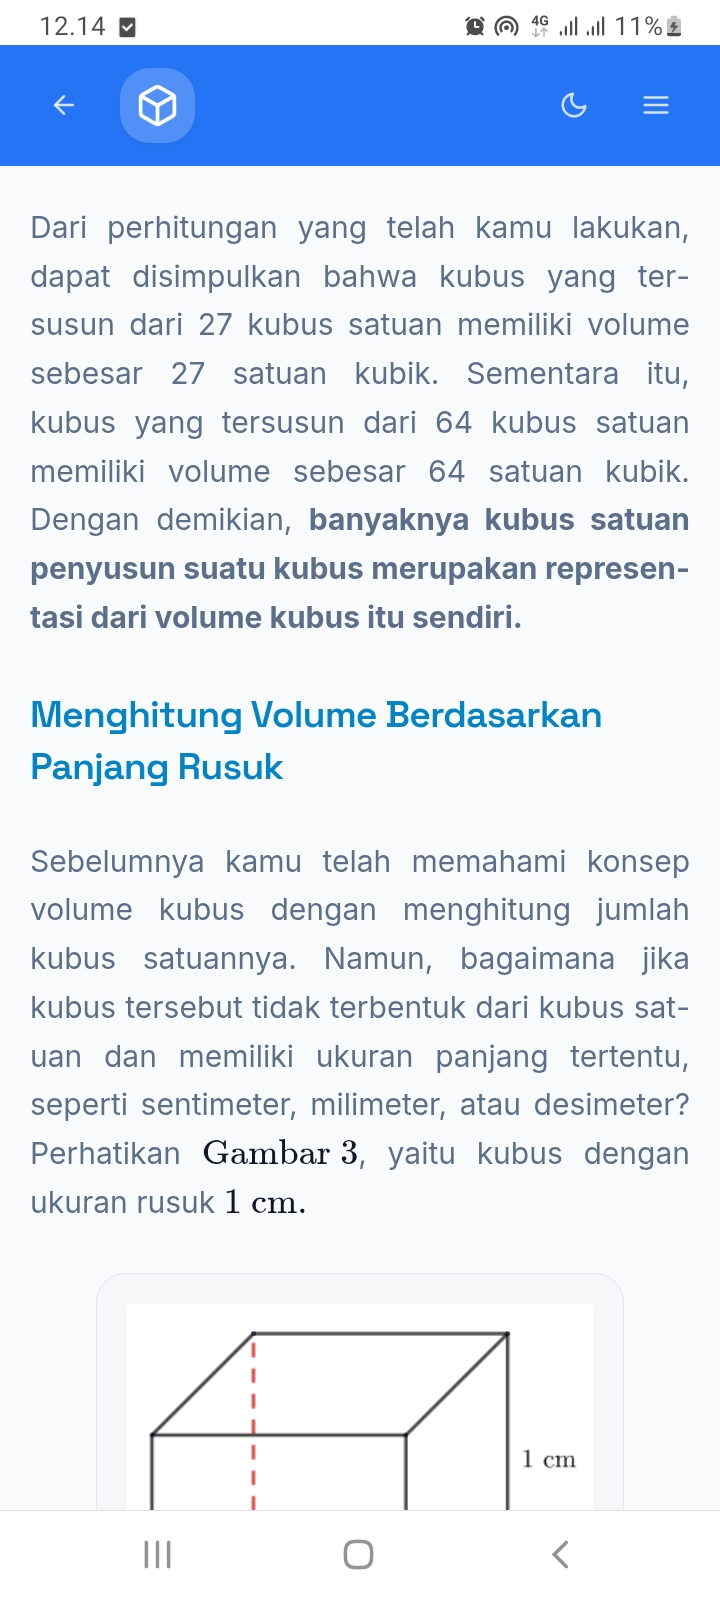
\includegraphics[width=0.25\textwidth]{revisi/sebelum/sebelumC.jpg} &
                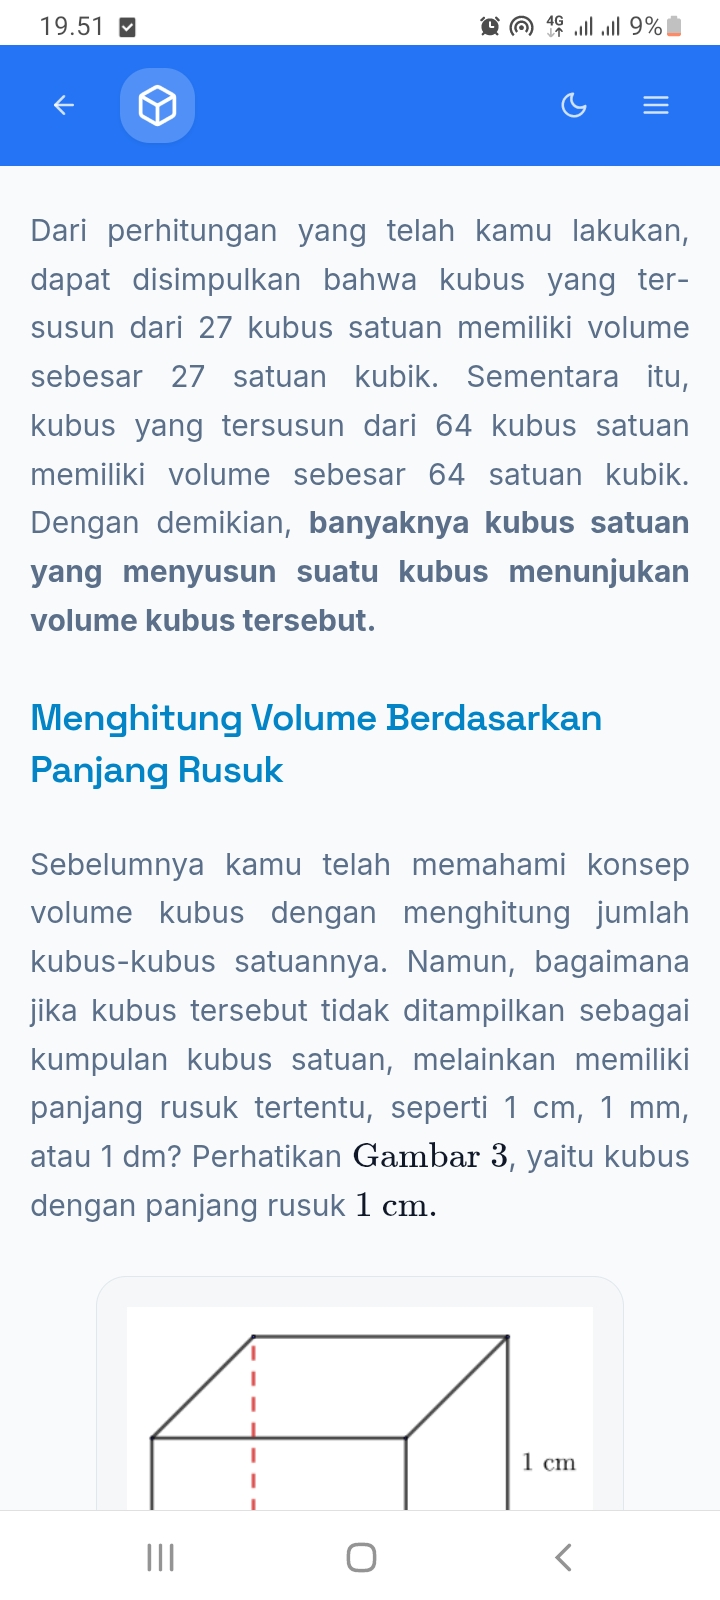
\includegraphics[width=0.25\textwidth]{revisi/sesudah/sesudahC.jpg} \\
            \end{tabular}
        \end{table}
        \item Memperbaiki definisi prisma.
        \begin{table}[H]
            \centering
            \begin{tabular}{c c}
                Sebelum Revisi & Sesudah Revisi \\
                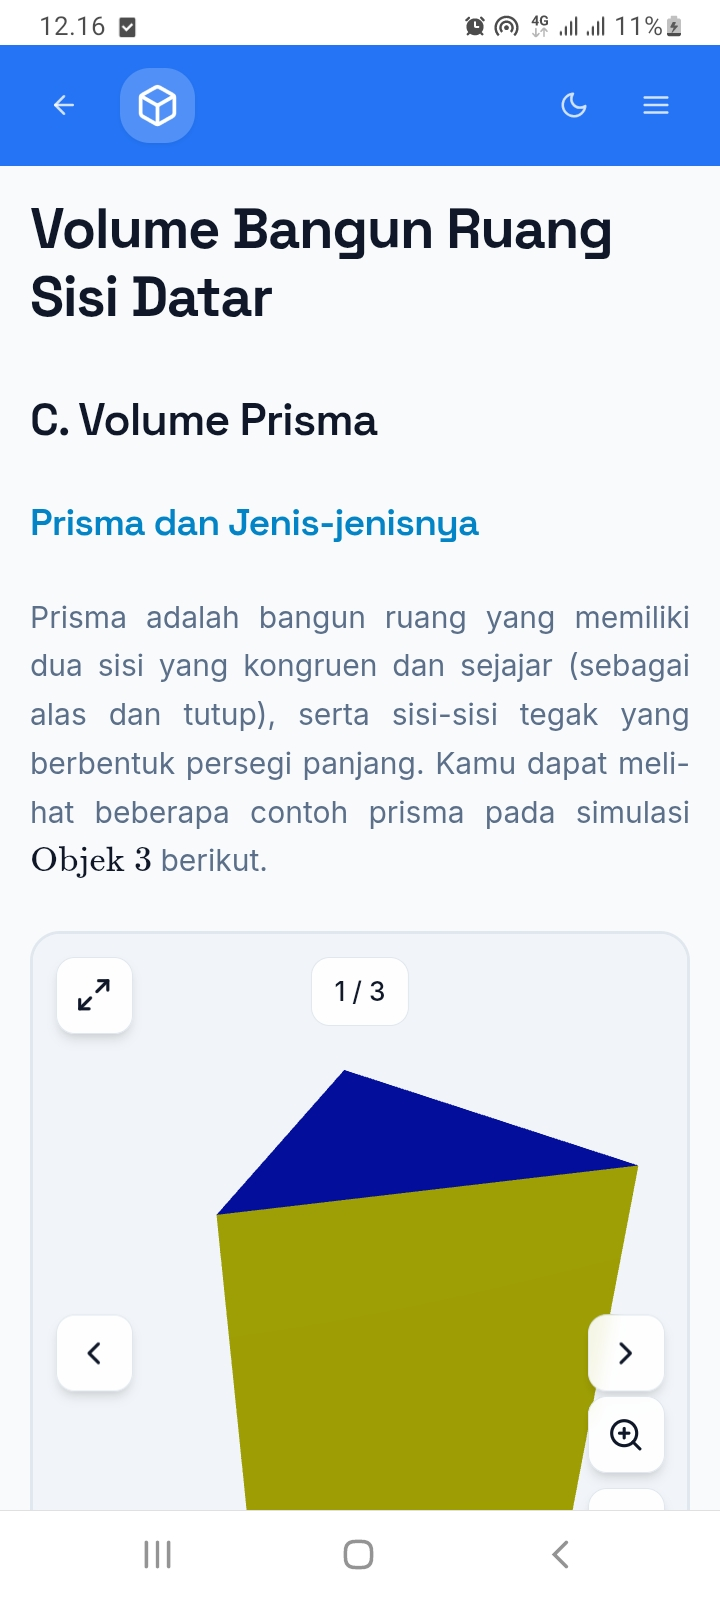
\includegraphics[width=0.25\textwidth]{revisi/sebelum/sebelumD.jpg} &
                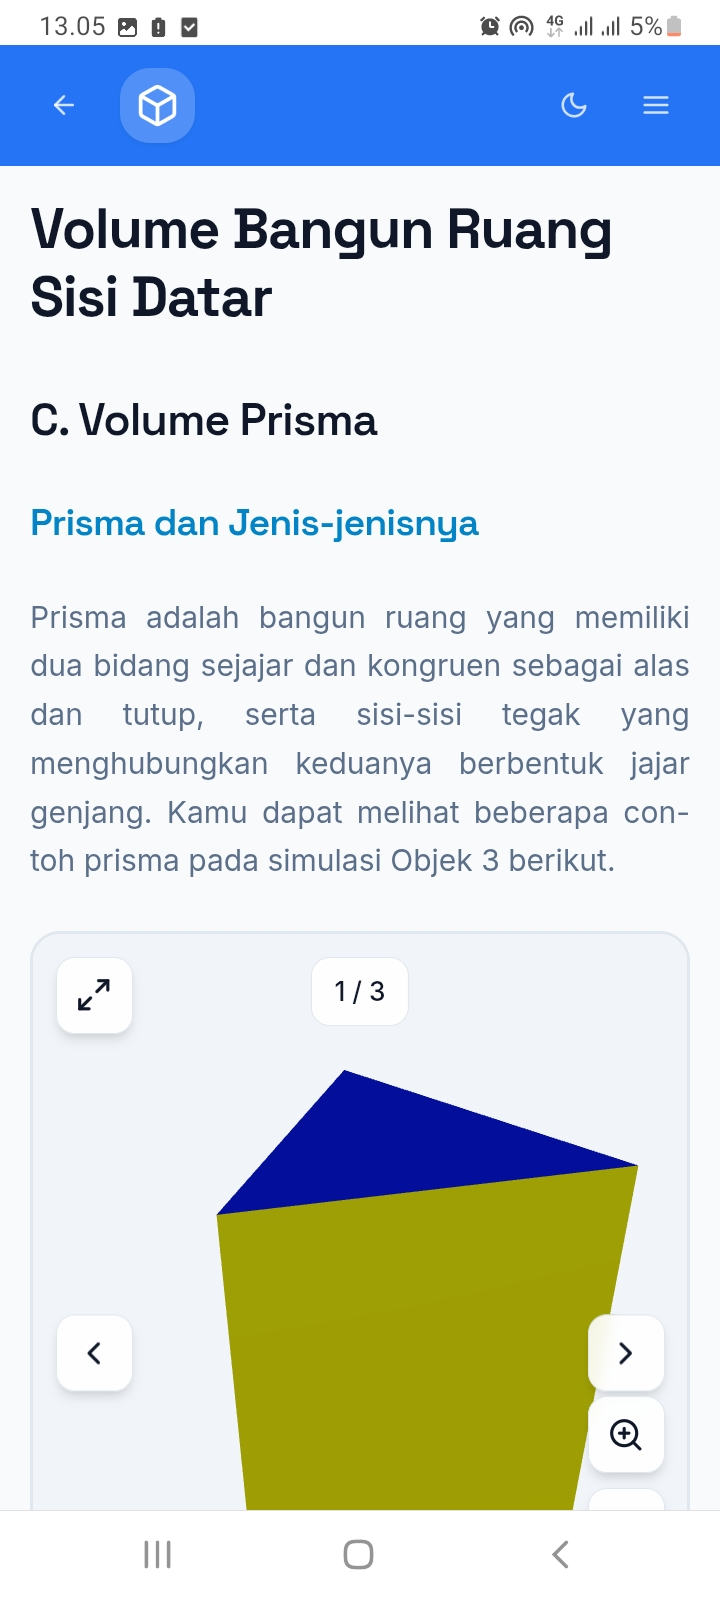
\includegraphics[width=0.25\textwidth]{revisi/sesudah/sesudahD.jpg} \\
            \end{tabular}
        \end{table}
        \item Menambahkan paragraf pengantar sebelum definisi jaring-jaring.
        \begin{table}[H]
            \centering
            \begin{tabular}{c c}
                Sebelum Revisi & Sesudah Revisi \\
                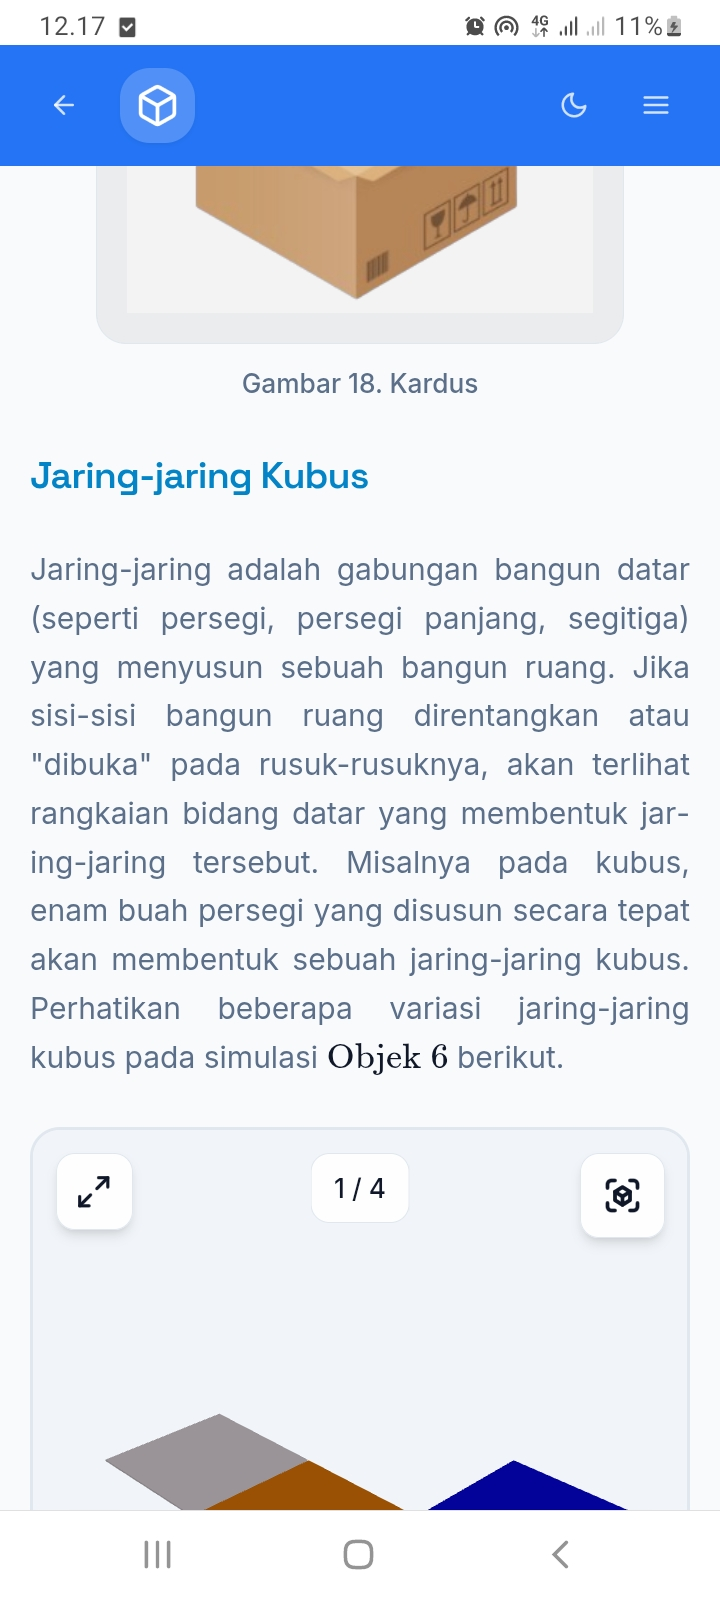
\includegraphics[width=0.25\textwidth]{revisi/sebelum/sebelumE.jpg} &
                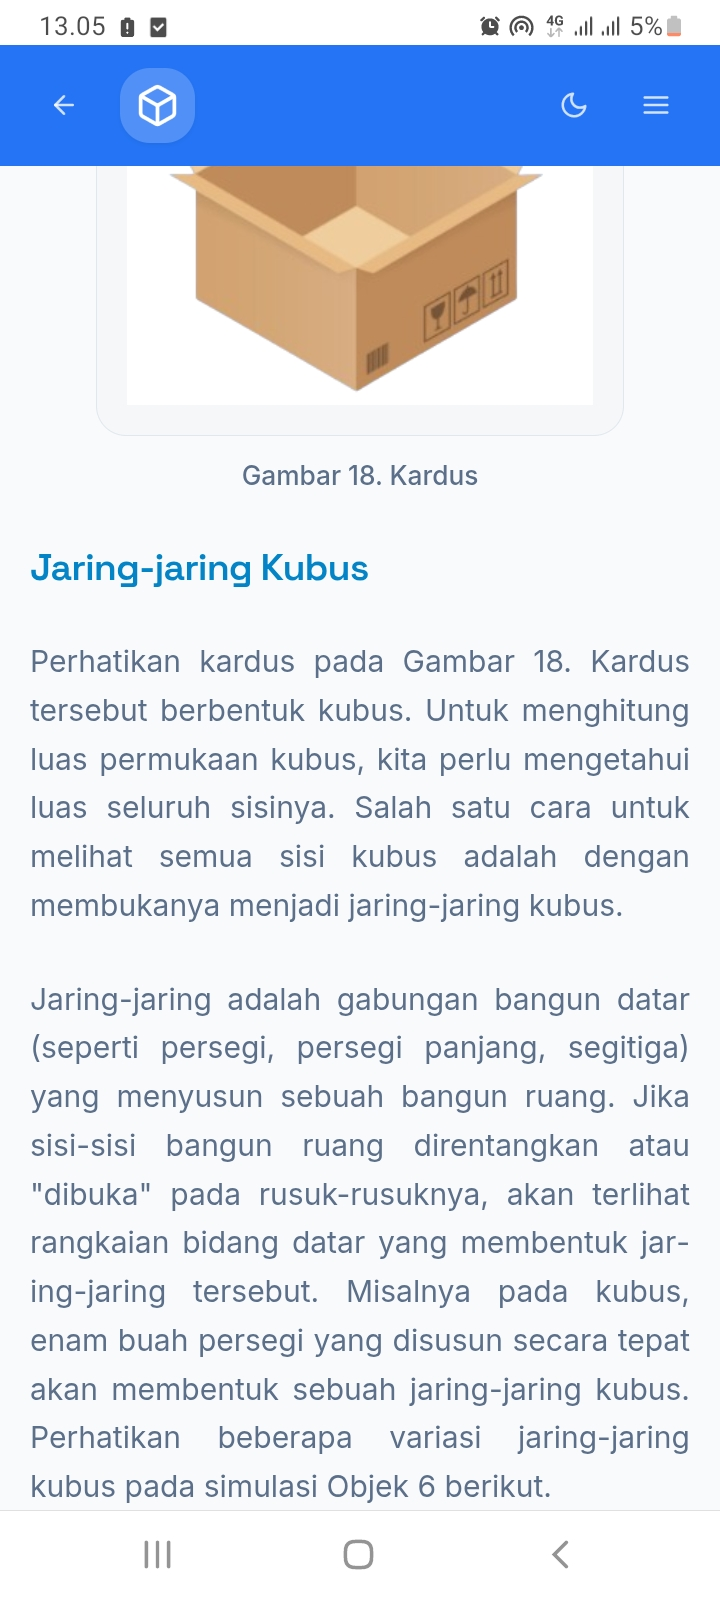
\includegraphics[width=0.25\textwidth]{revisi/sesudah/sesudahE.jpg} \\
            \end{tabular}
        \end{table}
        \item Menambah variasi jaring-jaring prisma.
        \begin{table}[H]
            \centering
            \begin{tabular}{c c}
                Sebelum Revisi & Sesudah Revisi \\
                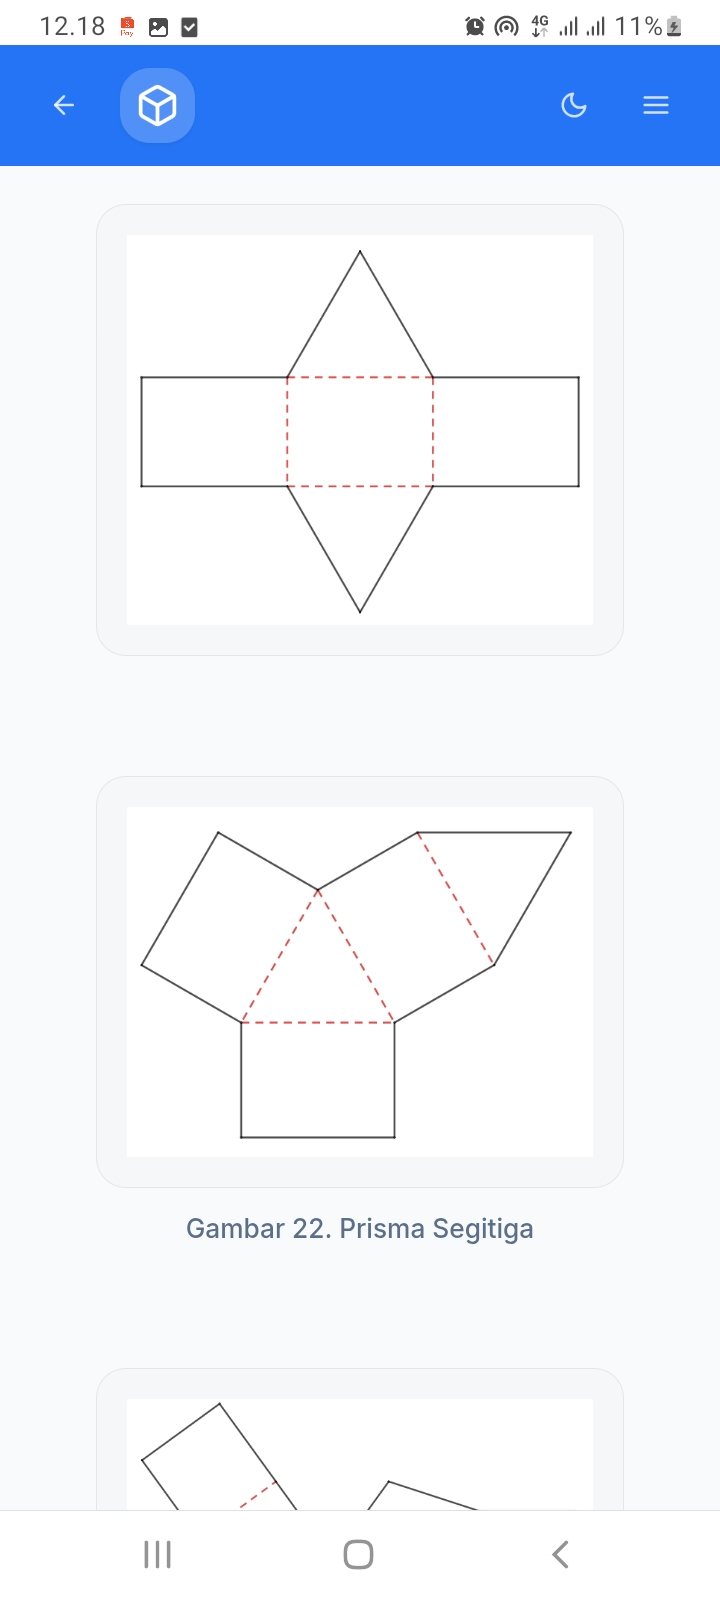
\includegraphics[width=0.25\textwidth]{revisi/sebelum/sebelumF.jpg} &
                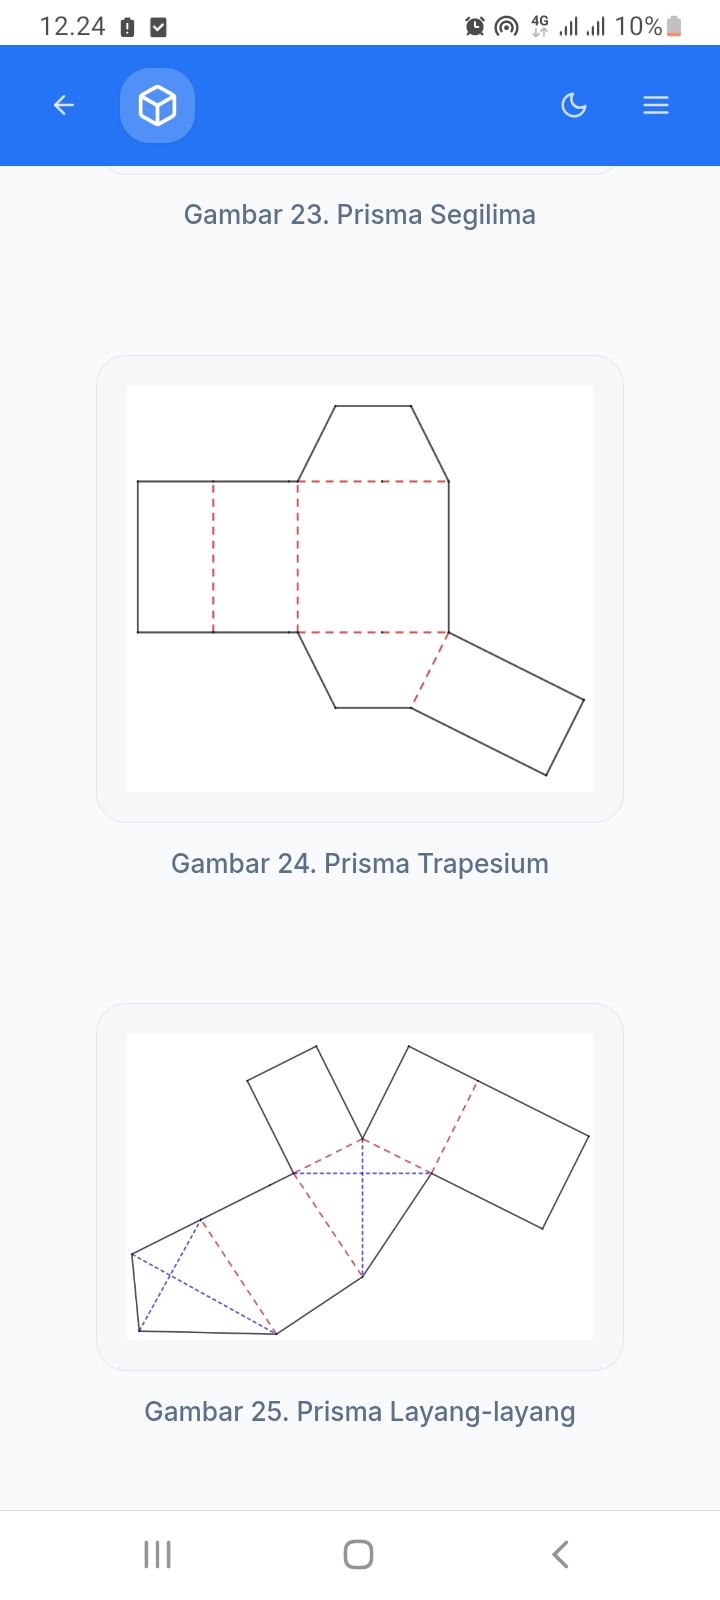
\includegraphics[width=0.25\textwidth]{revisi/sesudah/sesudahF.jpg} \\
            \end{tabular}
        \end{table}
        \item Menambahkan Capaian Pembelajaran, Indikator, dan Tujuan Pembelajaran.
        \begin{table}[H]
            \centering
            \begin{tabular}{c c c}
                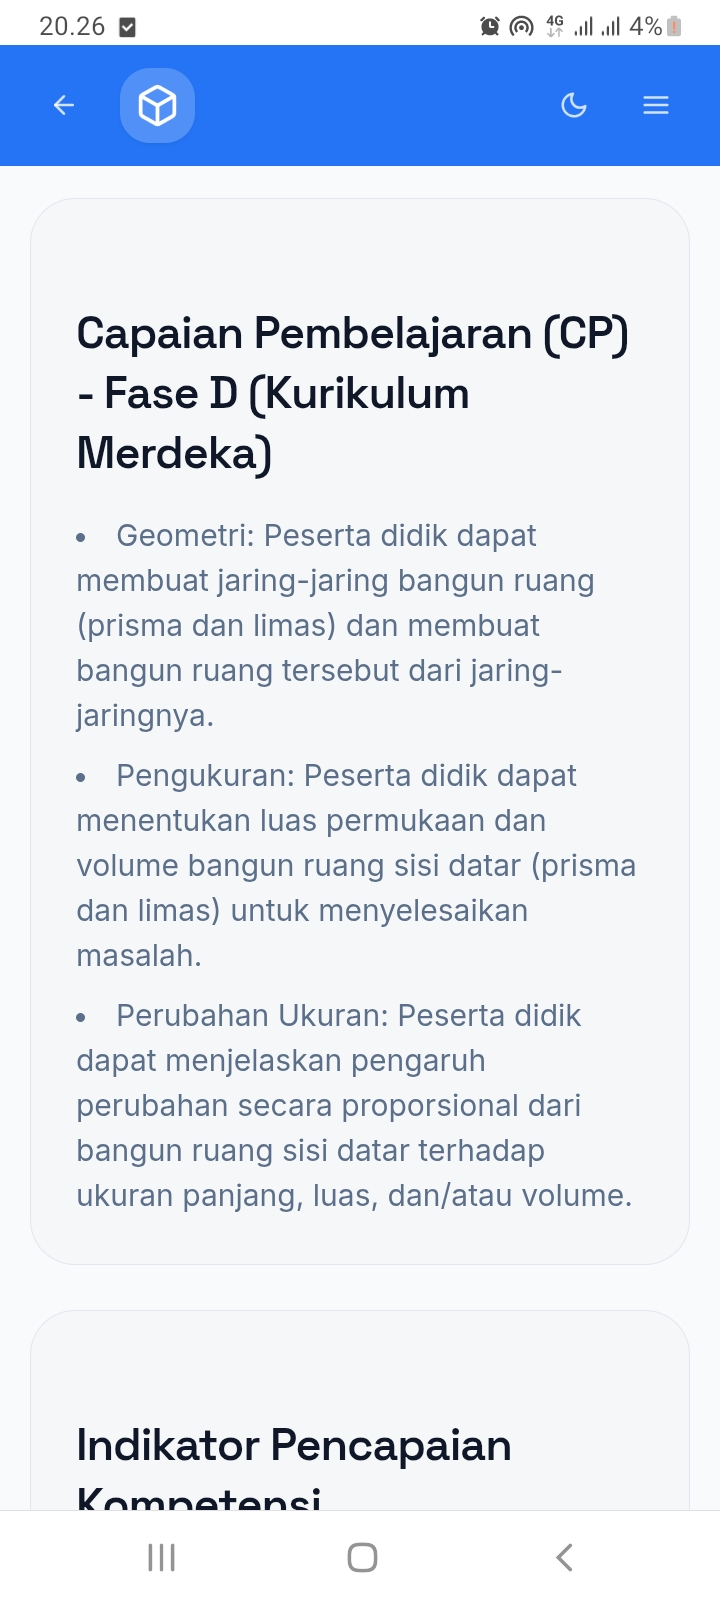
\includegraphics[width=0.25\textwidth]{revisi/sesudah/sesudahG1.jpg} &
                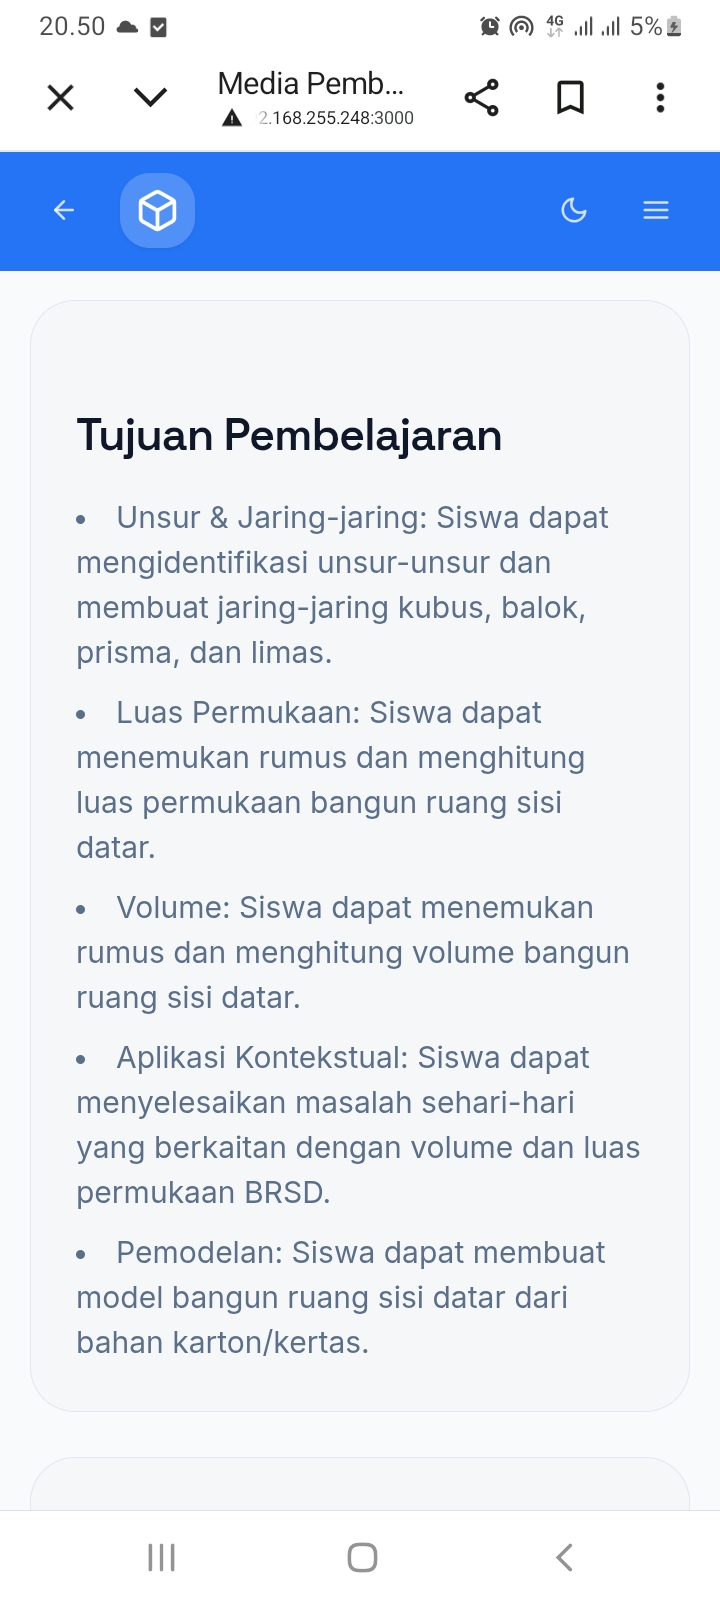
\includegraphics[width=0.25\textwidth]{revisi/sesudah/sesudahG2.jpg} &
                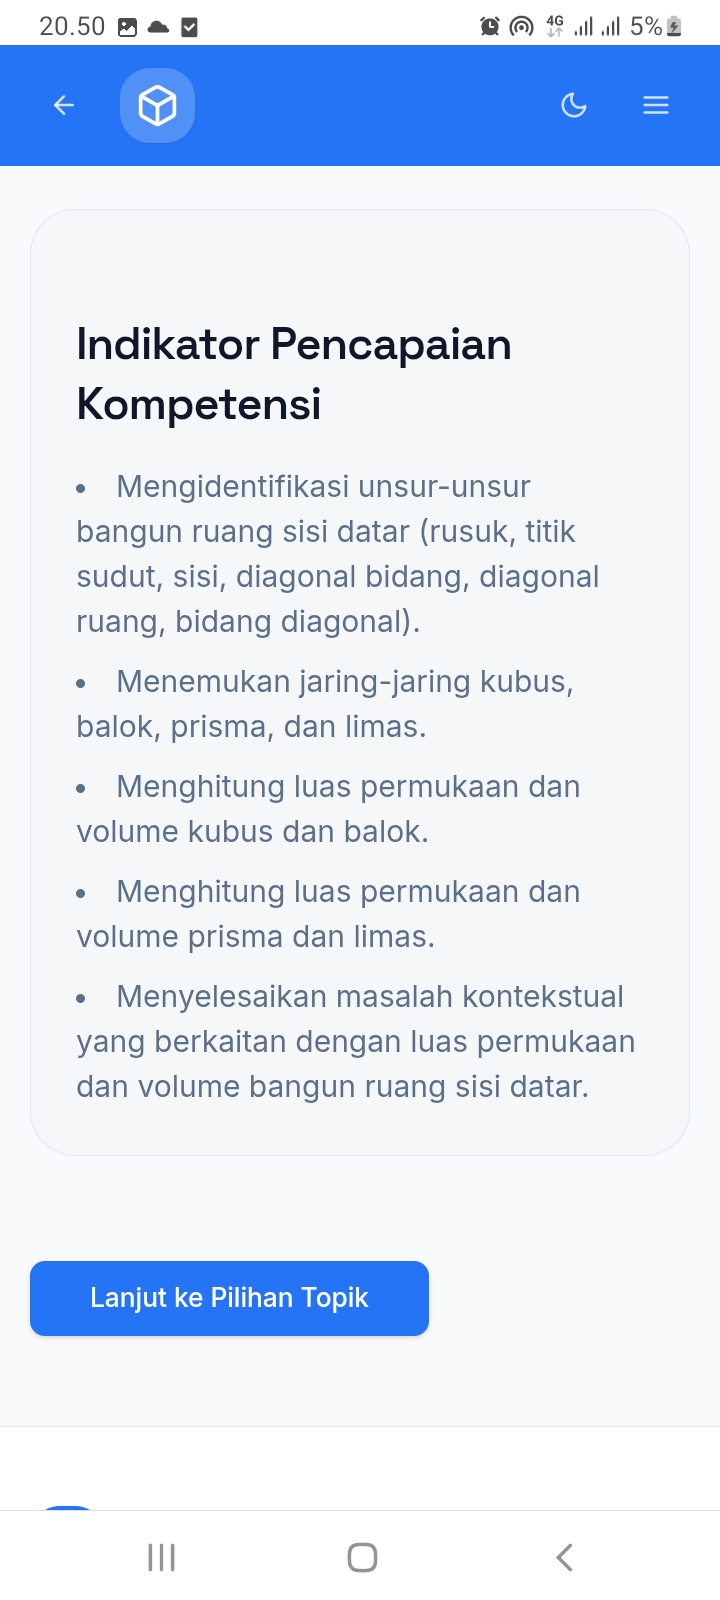
\includegraphics[width=0.25\textwidth]{revisi/sesudah/sesudahG3.jpg} \\
            \end{tabular}
        \end{table}
    \end{enumerate}
    \item Revisi Produk Hasil Validasi Ahli Media\\
    \hspace*{1cm}Ahli media hanya merekomendasikan perbaikan kunci jawaban yang salah.
    \begin{enumerate}
        \item Memperbaiki kunci jawaban.
        \begin{figure}[H]
            \centering
            \begin{tabular}{c c c}
                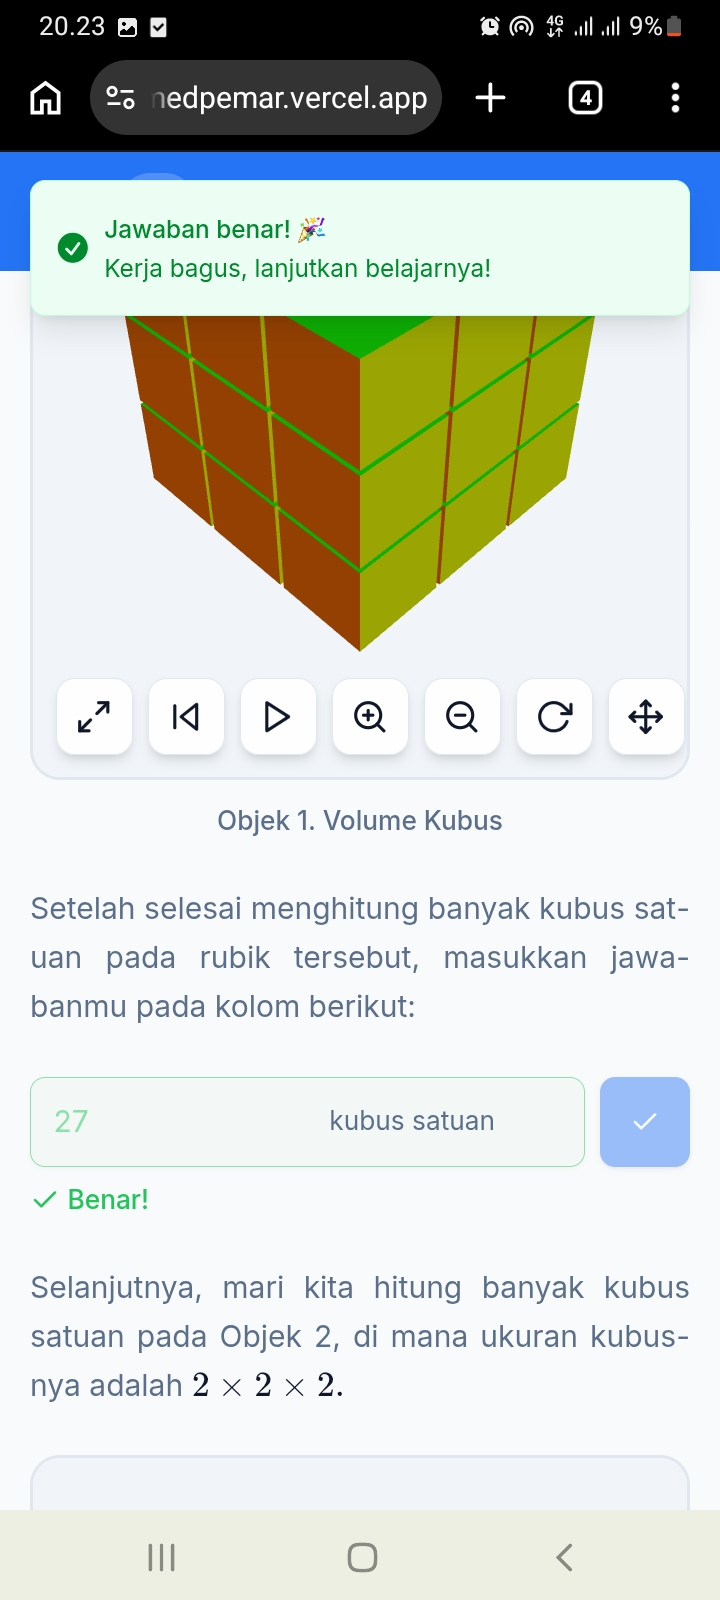
\includegraphics[width=0.25\textwidth]{revisi/Revisimedia2.jpg} &
                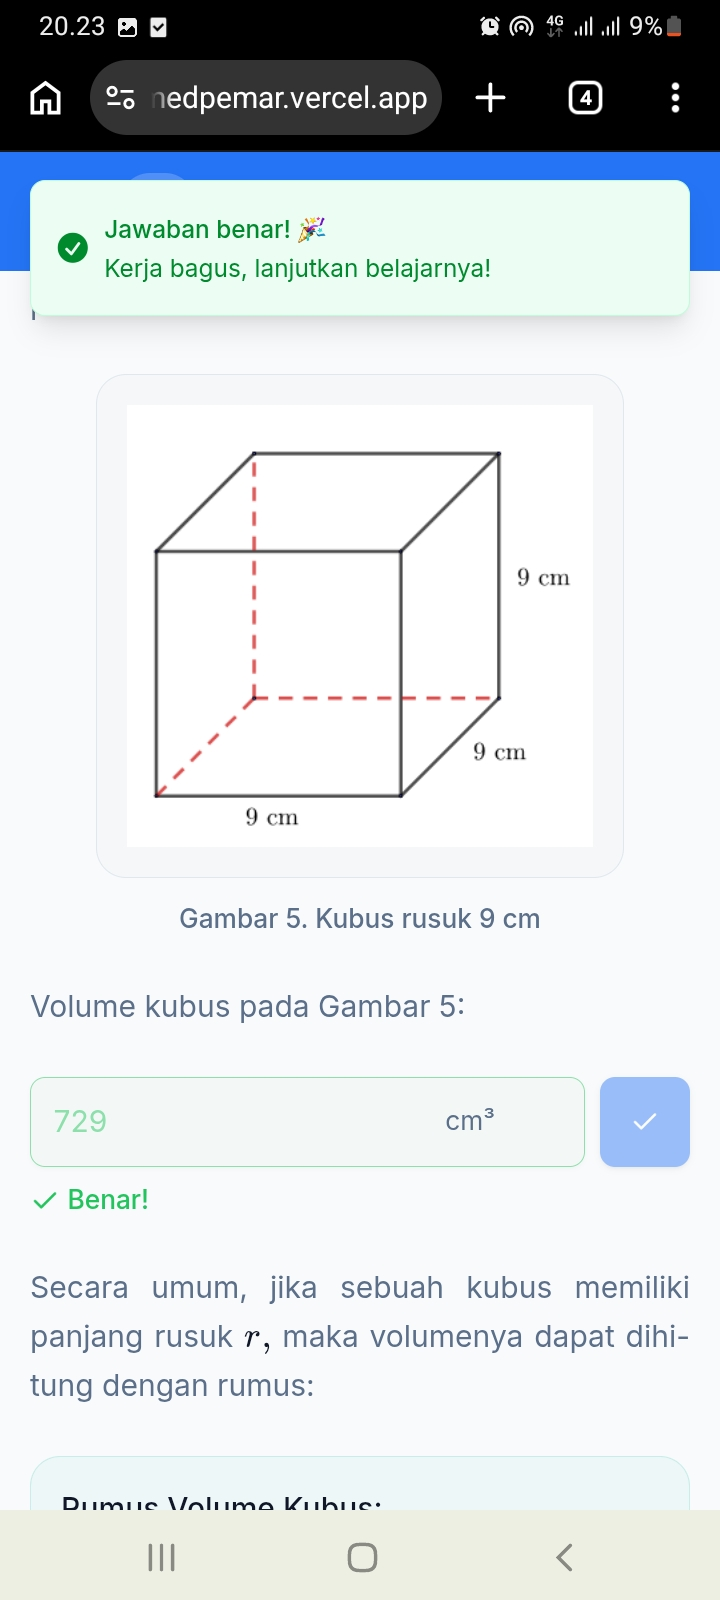
\includegraphics[width=0.25\textwidth]{revisi/Revisimedia.jpg} &
            \end{tabular}
            \caption{Contoh Perbaikan pada Kunci Jawaban}
        \end{figure}
    \end{enumerate}

    \item Revisi Produk Hasil Uji Coba Kelas Kecil\\
    \hspace*{1cm}Tidak ada saran revisi dari peserta didik.
\end{enumerate}

\textbf{D. Kajian Produk Akhir}
\addcontentsline{toc}{section}{D. Kajian Produk Akhir}

\hspace*{1cm}Media pembelajaran yang dikembangkan berupa \textit{website} dengan halaman awal (\textit{Landing Page}), halaman menu, halaman petunjuk, halaman materi, dan halaman kuis. Berikut penjelasan dan tampilan masing-masing halaman.
\begin{enumerate}
    \item Halaman Awal\\
    \hspace*{1cm}Halaman pertama saat mengakses https://medpemar.vercel.app. Menampilkan judul media, penjelasan singkat, cakupan isi, dan instansi pembuat. Berikut tampilan mode ponsel dan desktop.
    \begin{figure}[H]
        \centering
        \begin{tabular}{c c}
            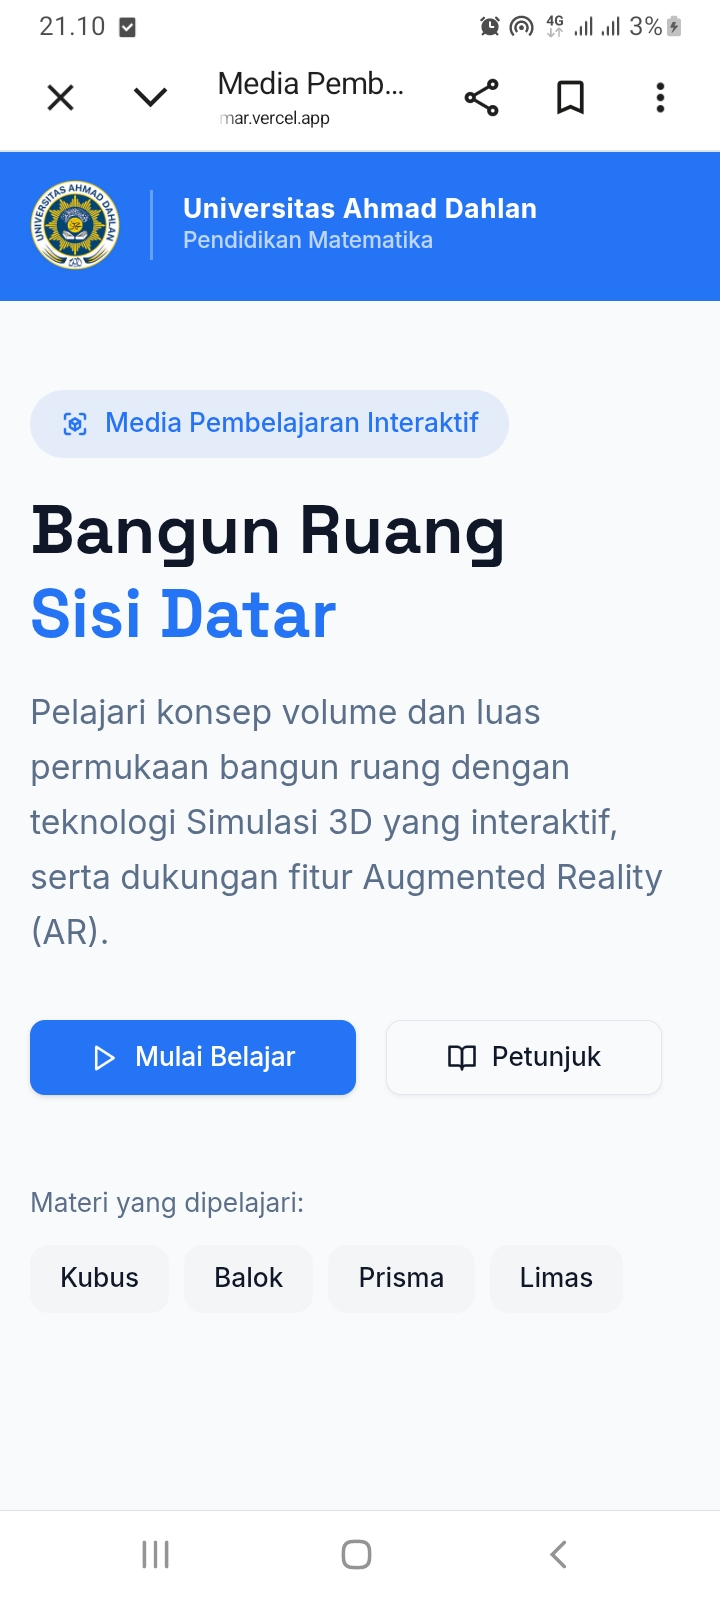
\includegraphics[width=0.25\textwidth]{revisi/Landingpage1.jpg} &
            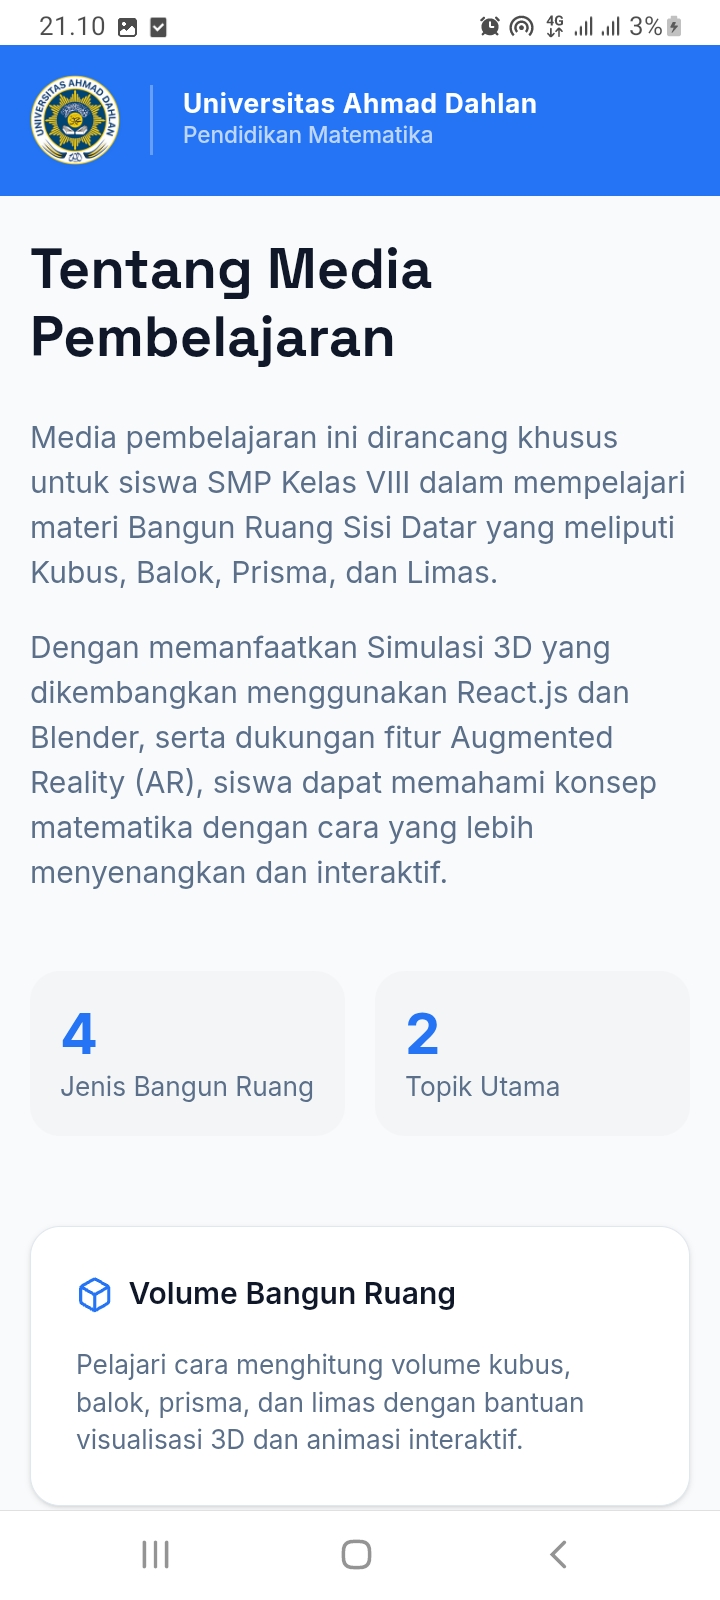
\includegraphics[width=0.25\textwidth]{revisi/Landingpage2.jpg} \\
        \end{tabular}
        \caption{\textit{Landing Page} versi Mobile}
    \end{figure}
    \begin{figure}[H]
        \centering
        \begin{tabular}{c}
            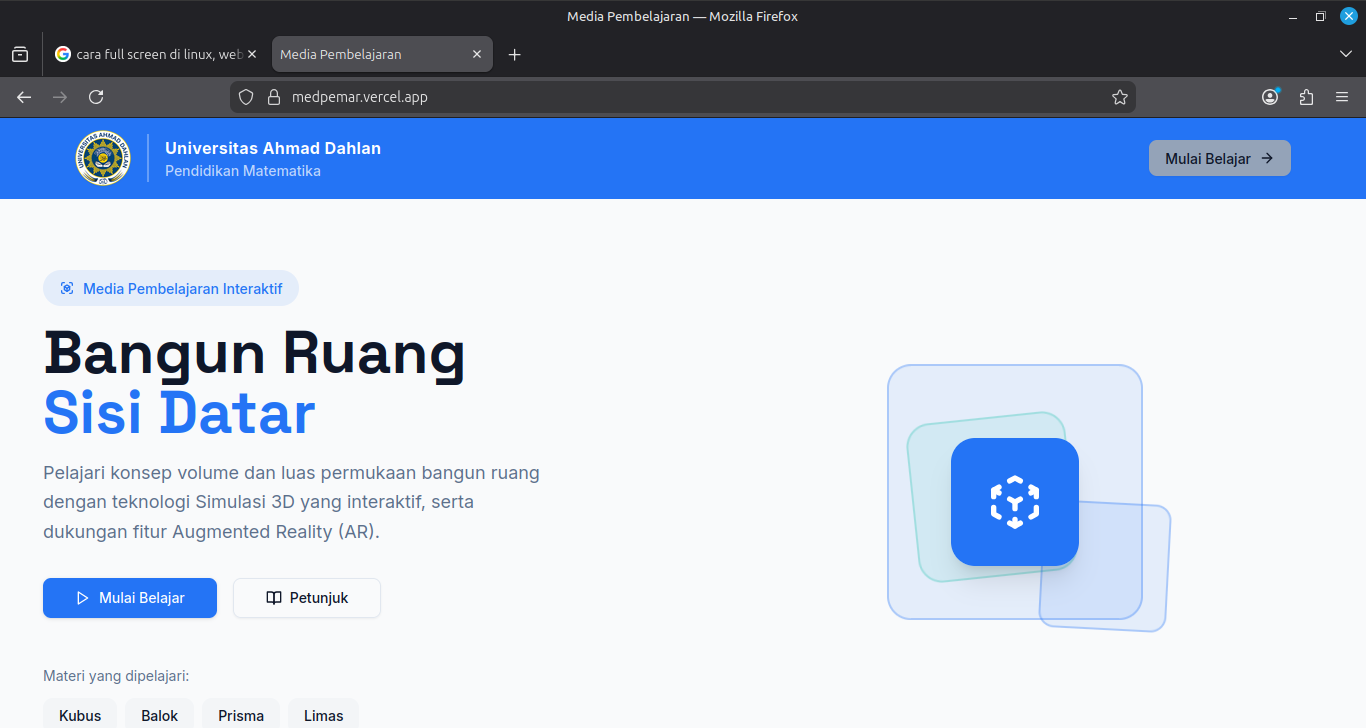
\includegraphics[width=1\textwidth]{revisi/Landingpage3.png} \\
        \end{tabular}
        \caption{\textit{Landing Page} versi Desktop}
    \end{figure}
    \item Halaman Pendahuluan Pembelajaran\\
    \hspace*{1cm}Berisi tujuan pembelajaran, capaian pembelajaran, dan indikator pencapaian kompetensi.
    \begin{figure}[H]
        \centering
        \begin{tabular}{c c c}
            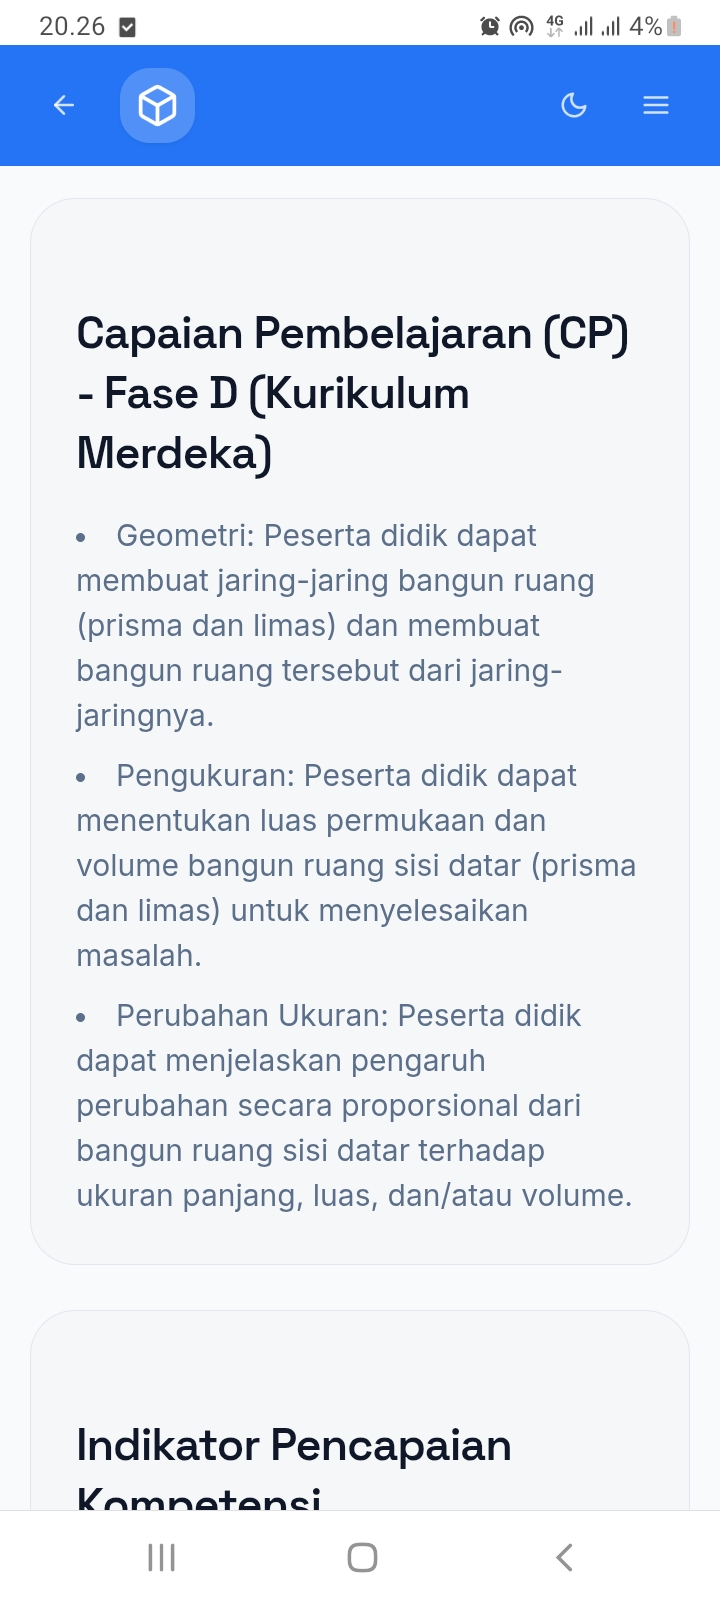
\includegraphics[width=0.3\textwidth]{revisi/sesudah/sesudahG1.jpg} &
            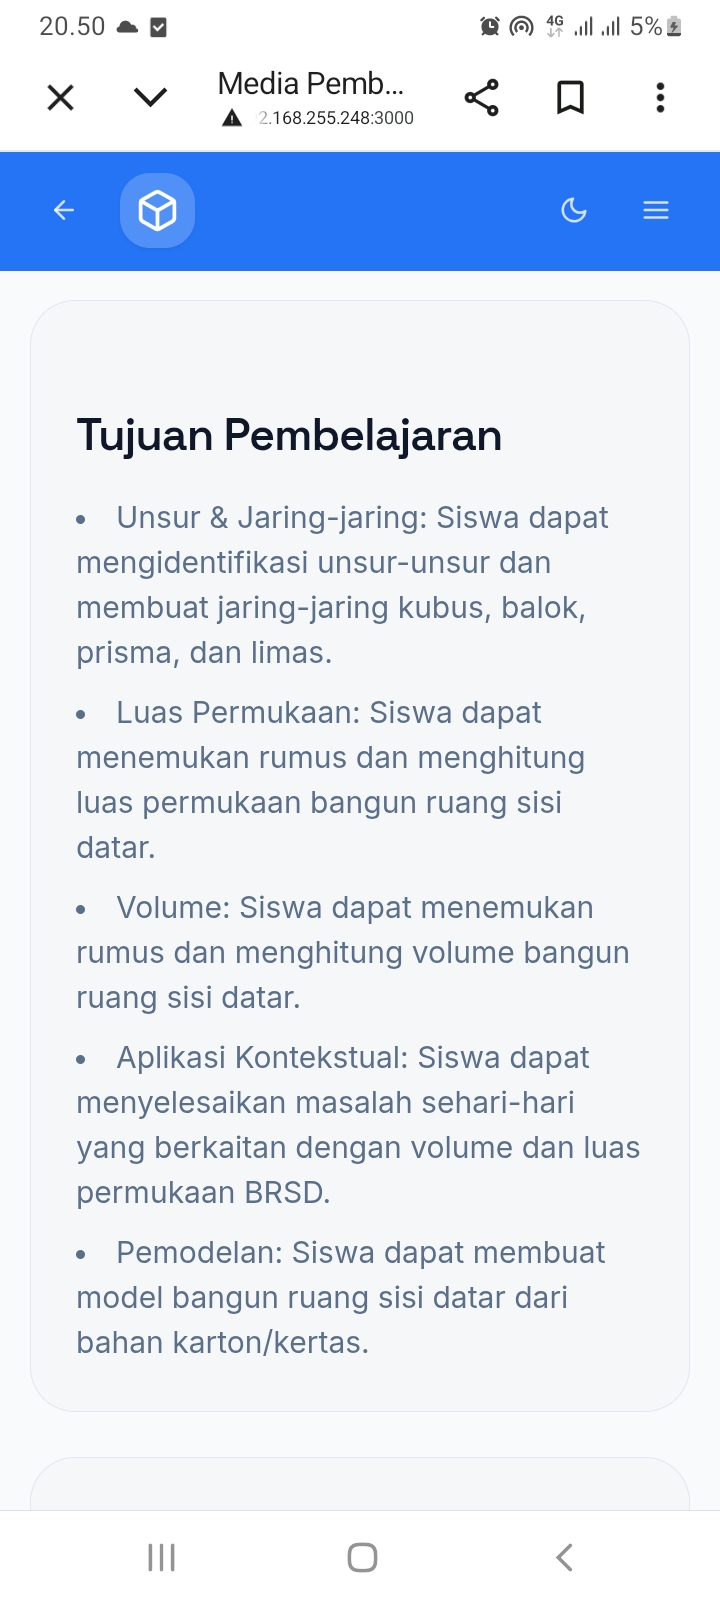
\includegraphics[width=0.3\textwidth]{revisi/sesudah/sesudahG2.jpg} &
            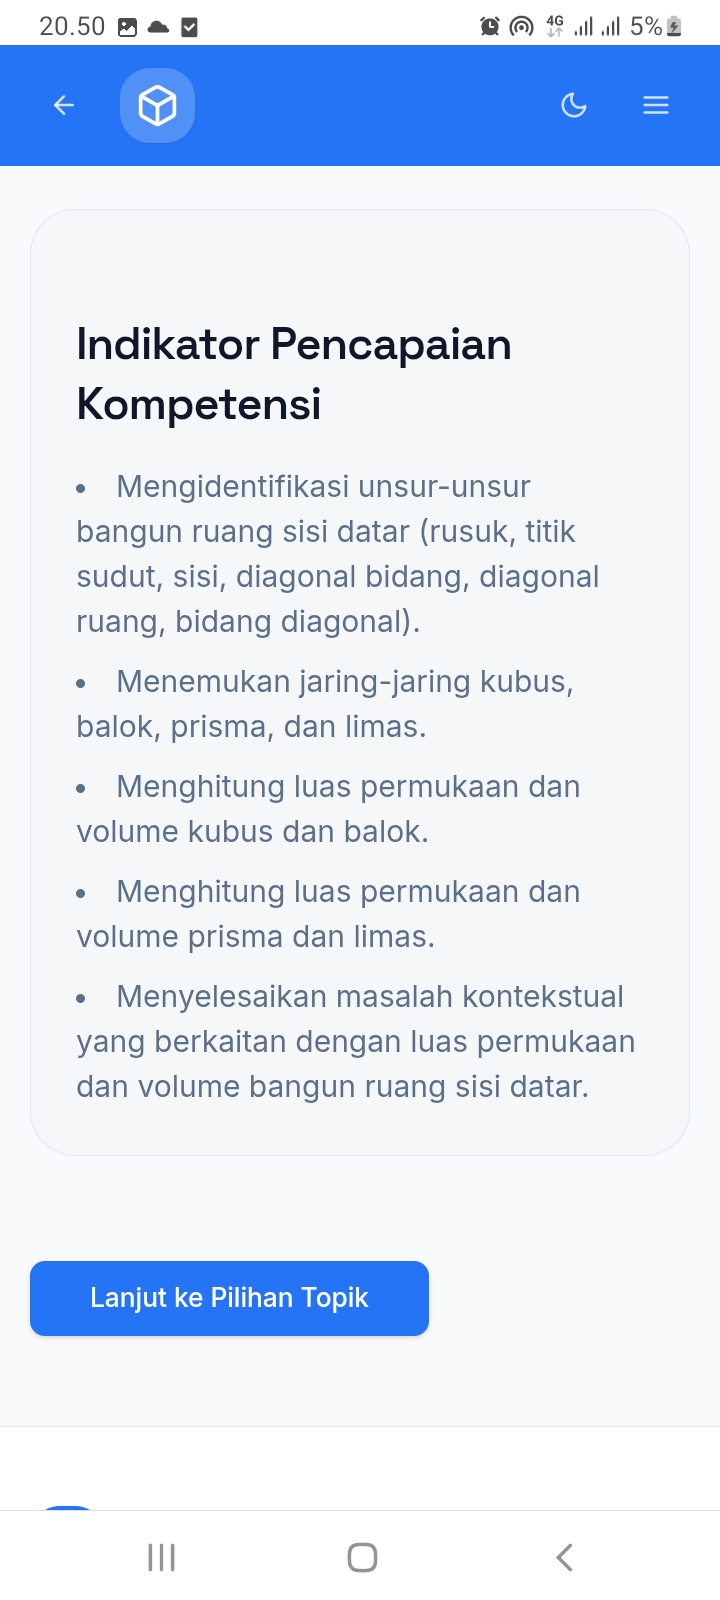
\includegraphics[width=0.3\textwidth]{revisi/sesudah/sesudahG3.jpg} \\
        \end{tabular}
        \caption{Halaman Pendahuluan Pembelajaran}
    \end{figure}
    \item Halaman Menu\\
    \hspace*{1cm}Berisi pilihan materi, latihan soal, dan unduh barcode untuk simulasi 3D.
    \begin{figure}[H]
        \centering
        \begin{tabular}{c c c}
            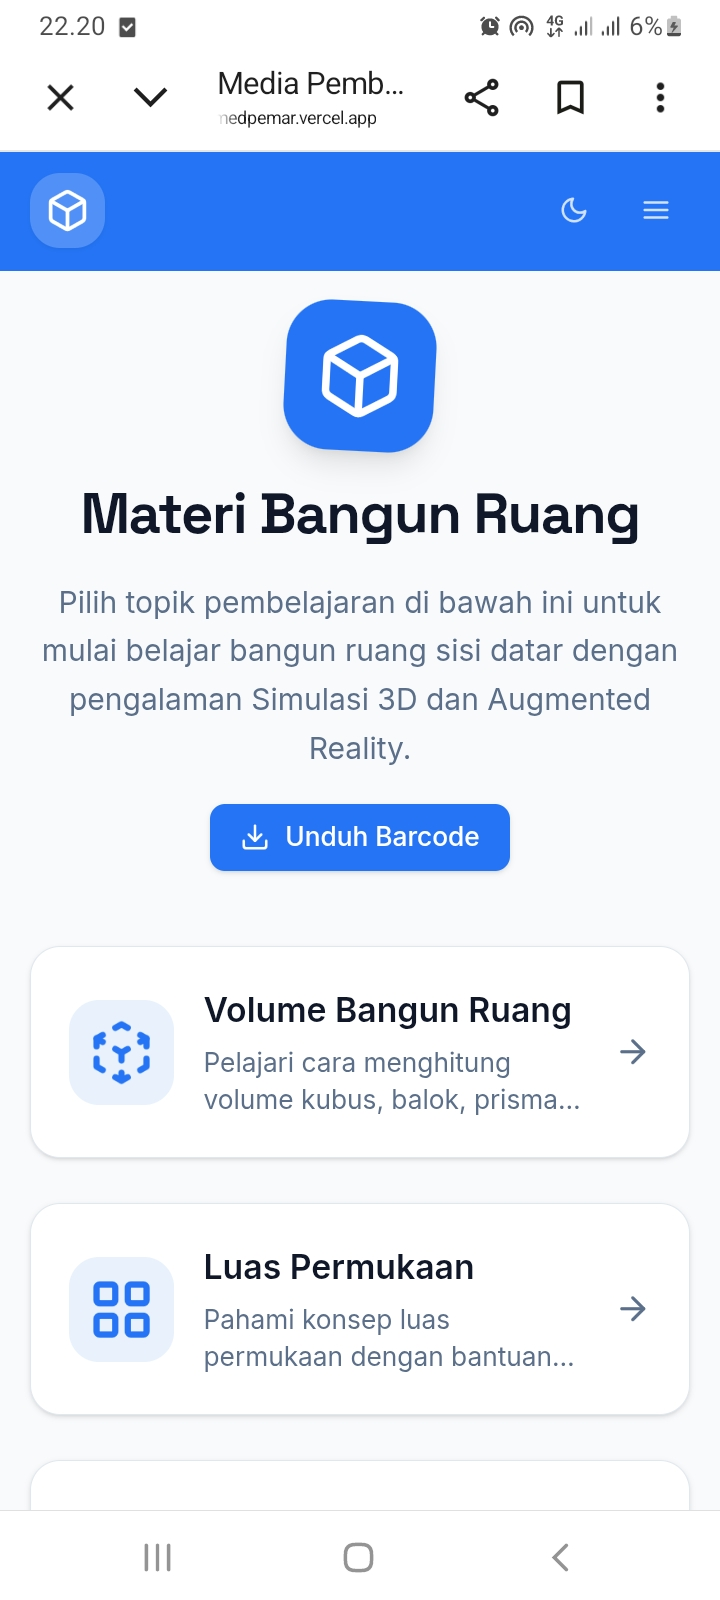
\includegraphics[width=0.3\textwidth]{revisi/Menu.jpg} &
            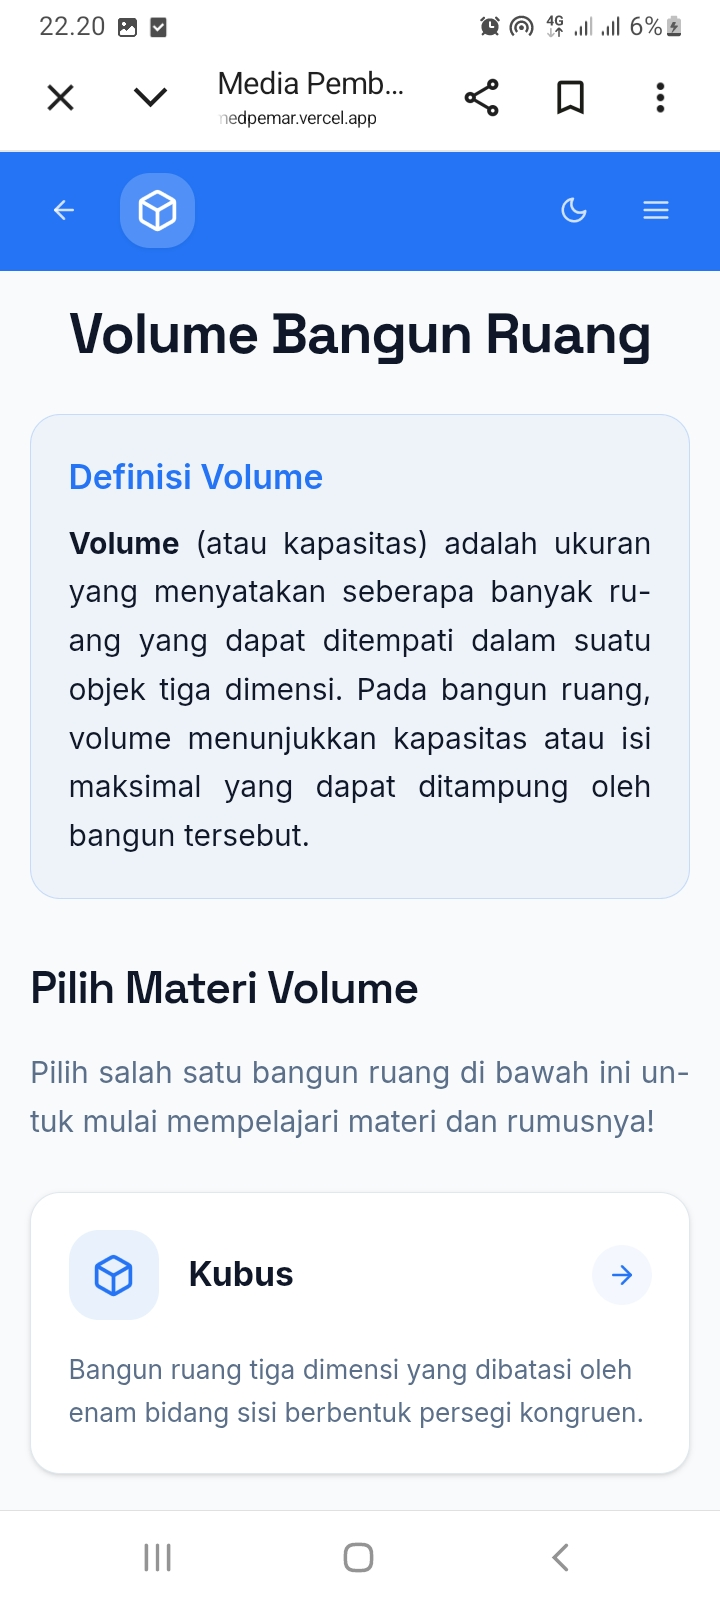
\includegraphics[width=0.3\textwidth]{revisi/Menuvolume.jpg} &
            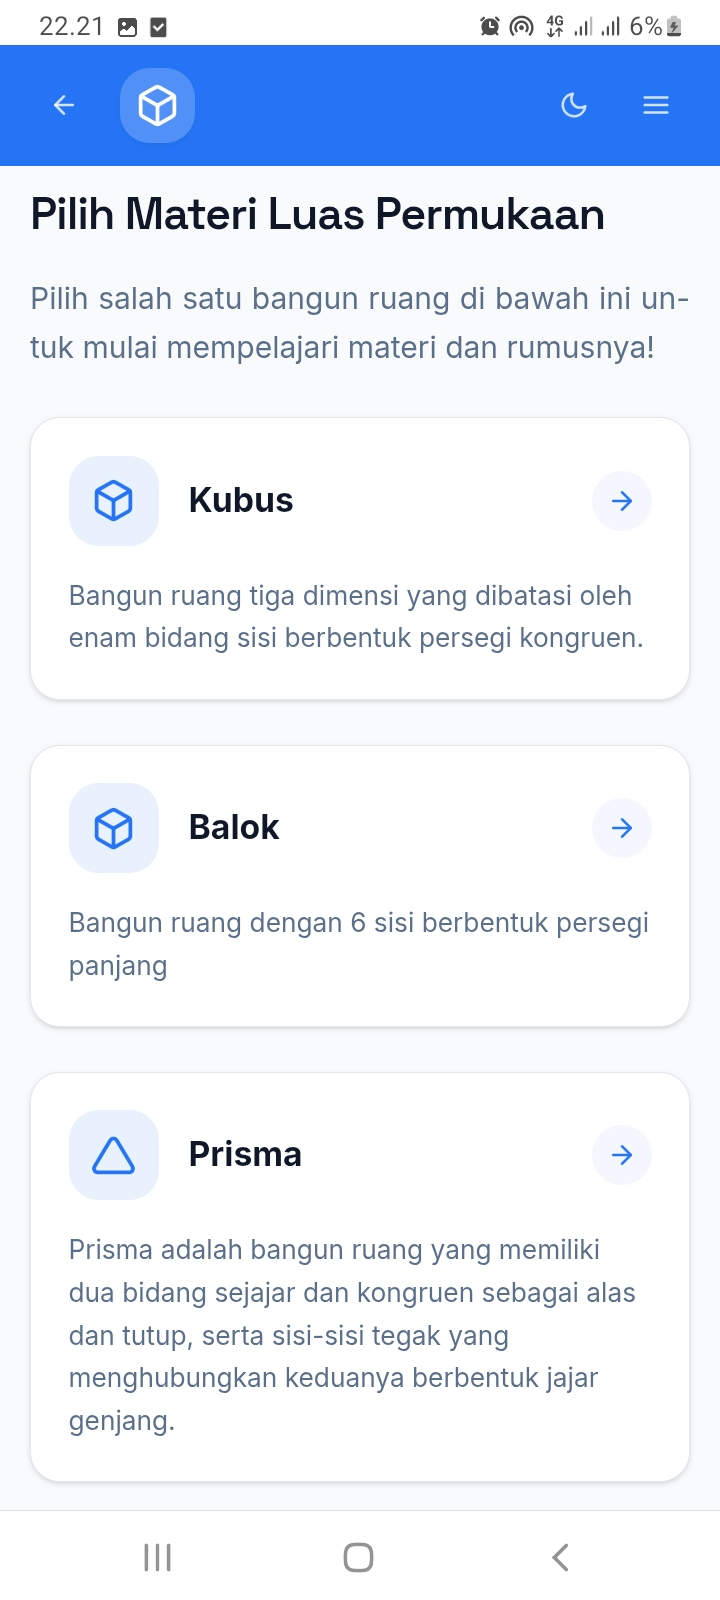
\includegraphics[width=0.3\textwidth]{revisi/Menuluaspermukaan.jpg} \\
        \end{tabular}
        \caption{Halaman Menu}
    \end{figure}

    \item Halaman Materi\\
    \hspace*{1cm}Peserta didik mempelajari volume dan luas permukaan bangun ruang melalui tampilan 3D dan simulasi. Tersedia latihan soal dan pembahasan di akhir setiap bab.
    \begin{figure}[H]
        \centering
        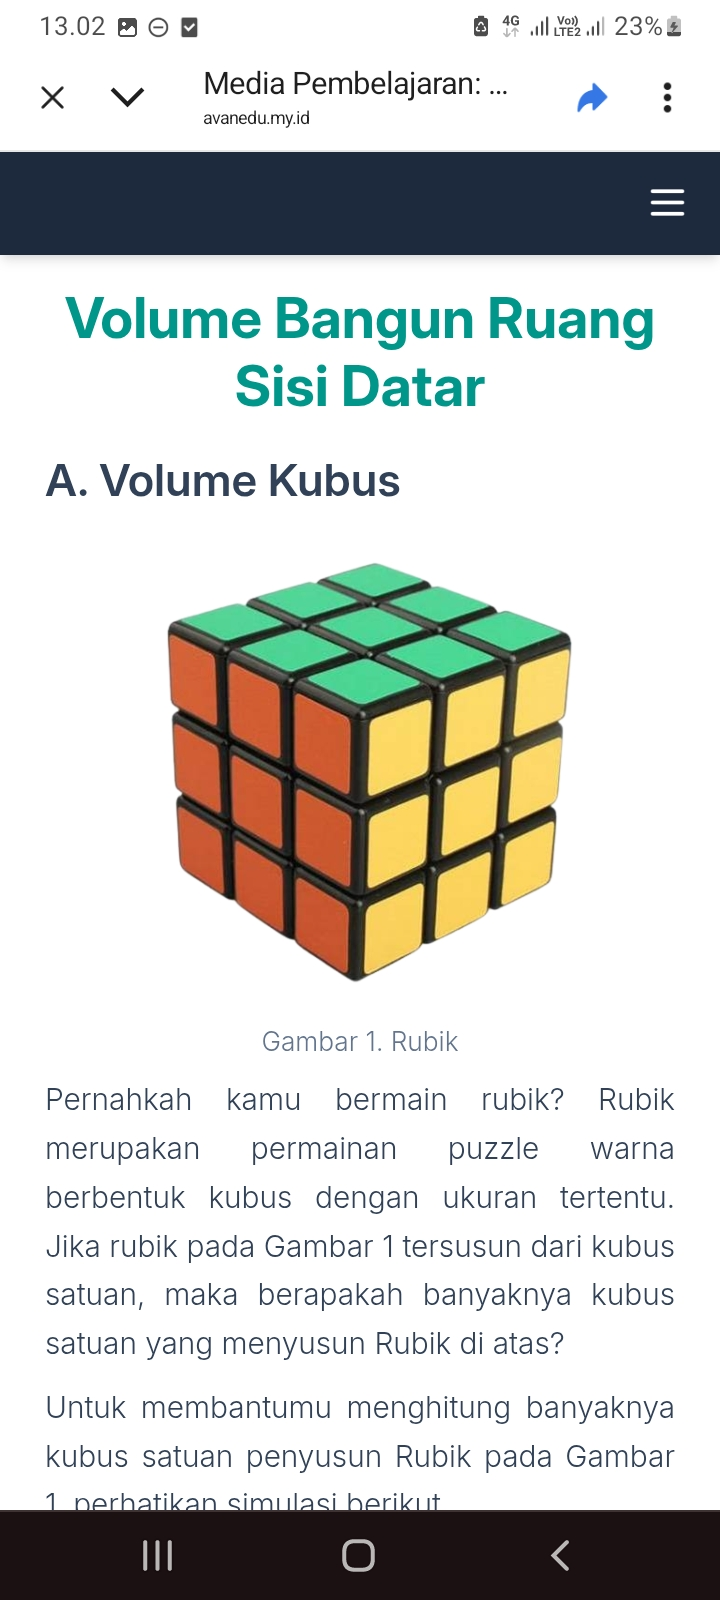
\includegraphics[width=0.2\textwidth]{images/materi1.jpg}
        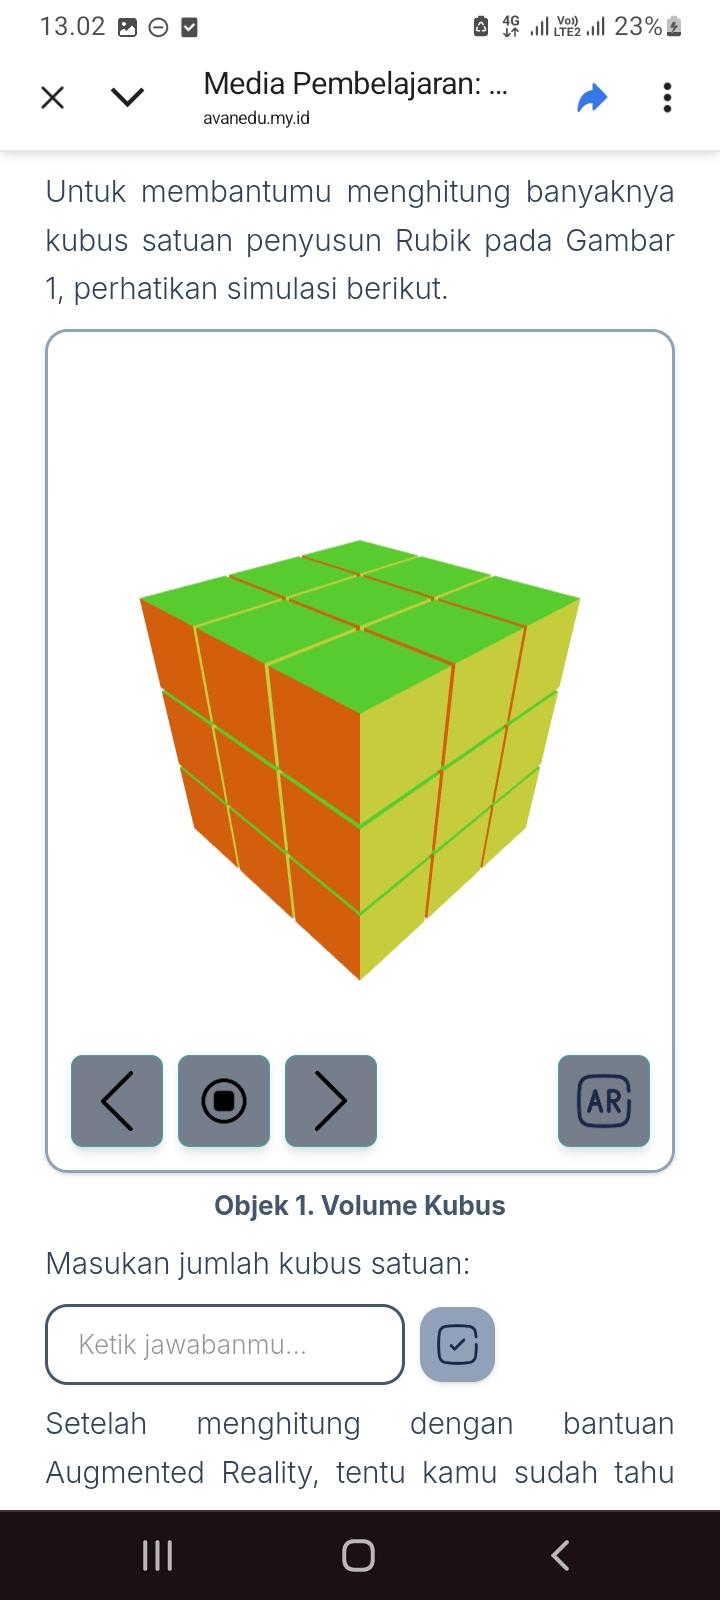
\includegraphics[width=0.2\textwidth]{images/materi2.jpg}
        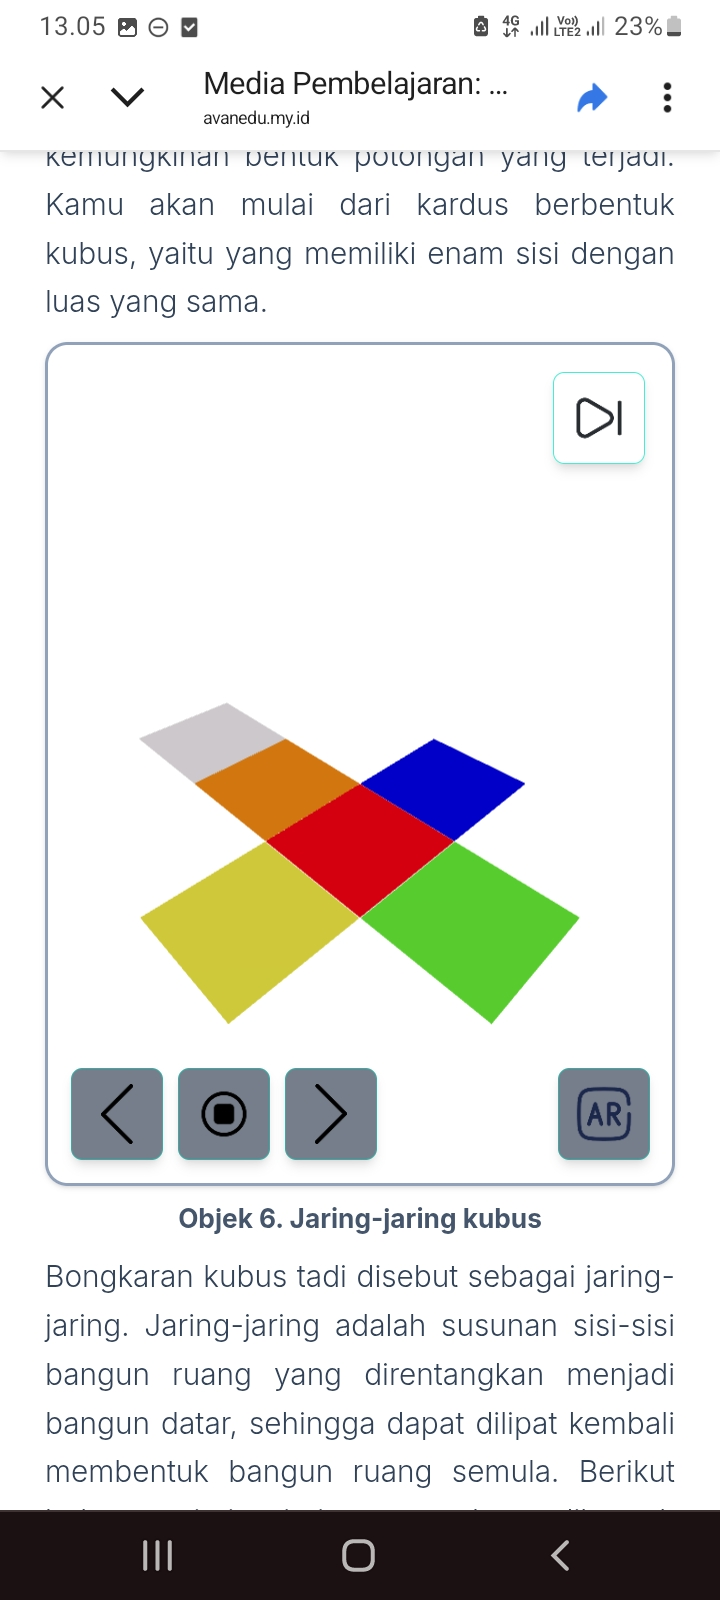
\includegraphics[width=0.2\textwidth]{images/materi3.jpg}
        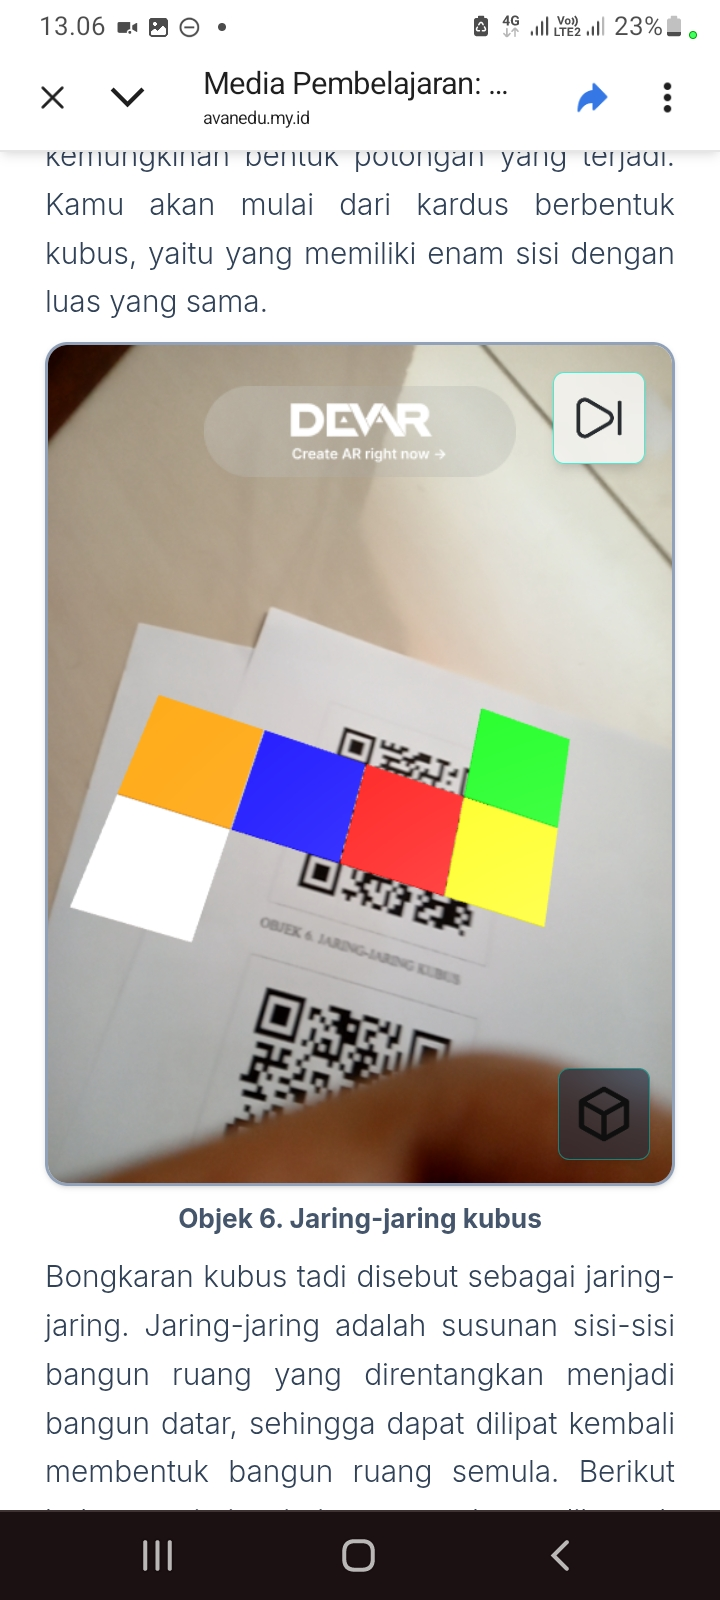
\includegraphics[width=0.2\textwidth]{images/materi4.jpg}
        \caption{Halaman Materi}
        \label{fig:materi}
    \end{figure}

    \item Halaman Kuis\\
    \hspace*{1cm}Disajikan lima soal dengan timer 30 menit. Peserta didik memasukkan kode ujian, menjawab soal, dan dapat menyisipkan foto.
    \begin{figure}[H]
        \centering
        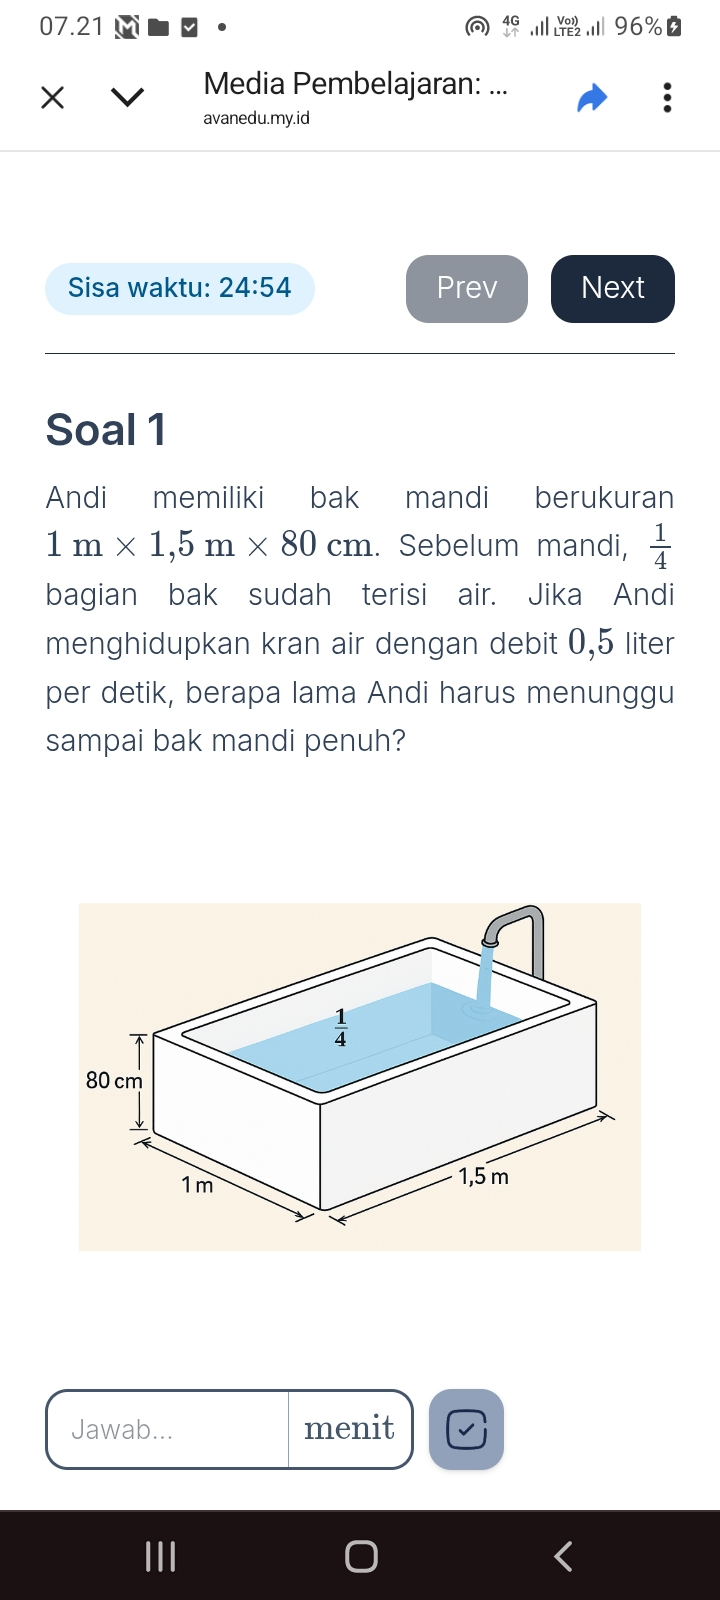
\includegraphics[width=0.25\textwidth]{images/kuis1.jpg}
        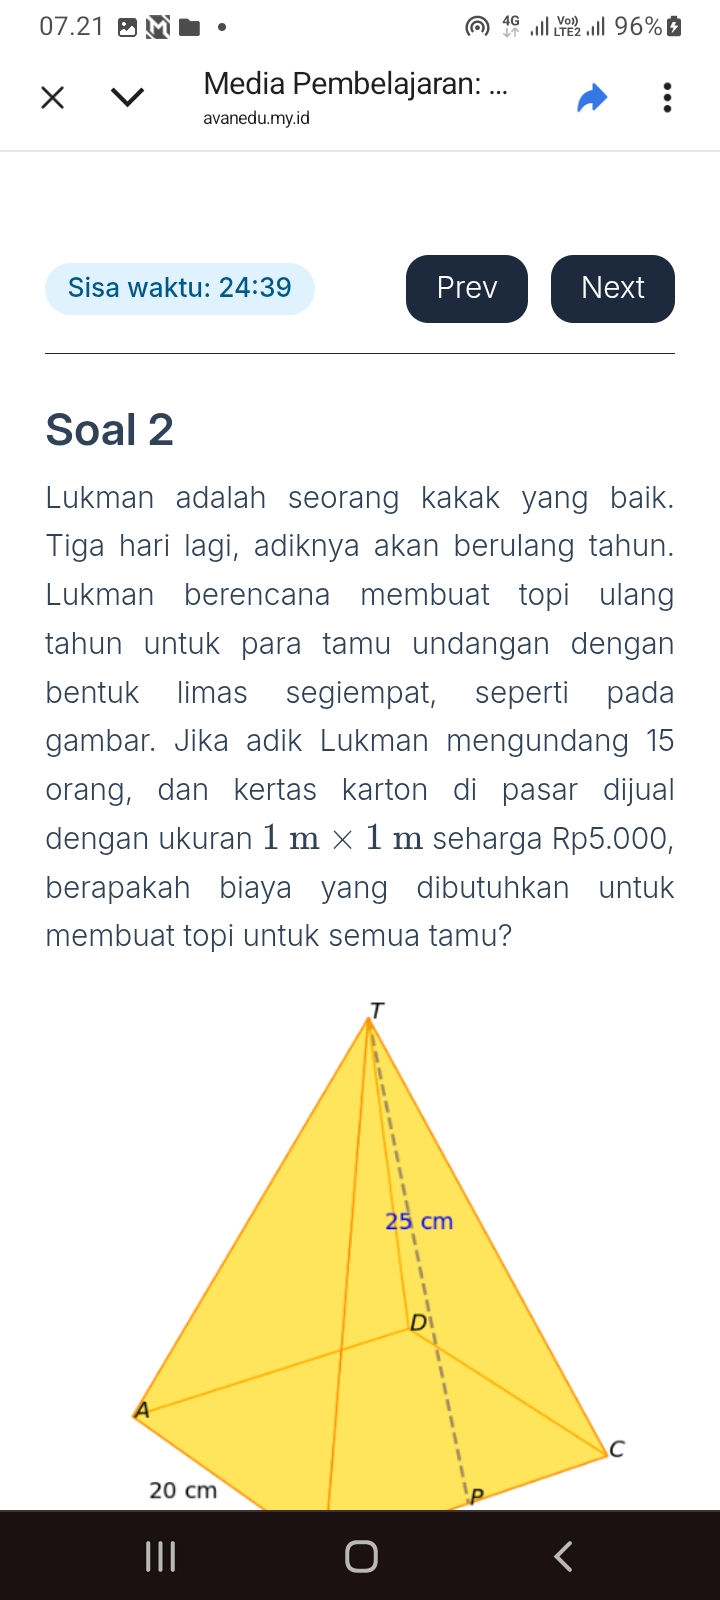
\includegraphics[width=0.25\textwidth]{images/kuis2.jpg}
        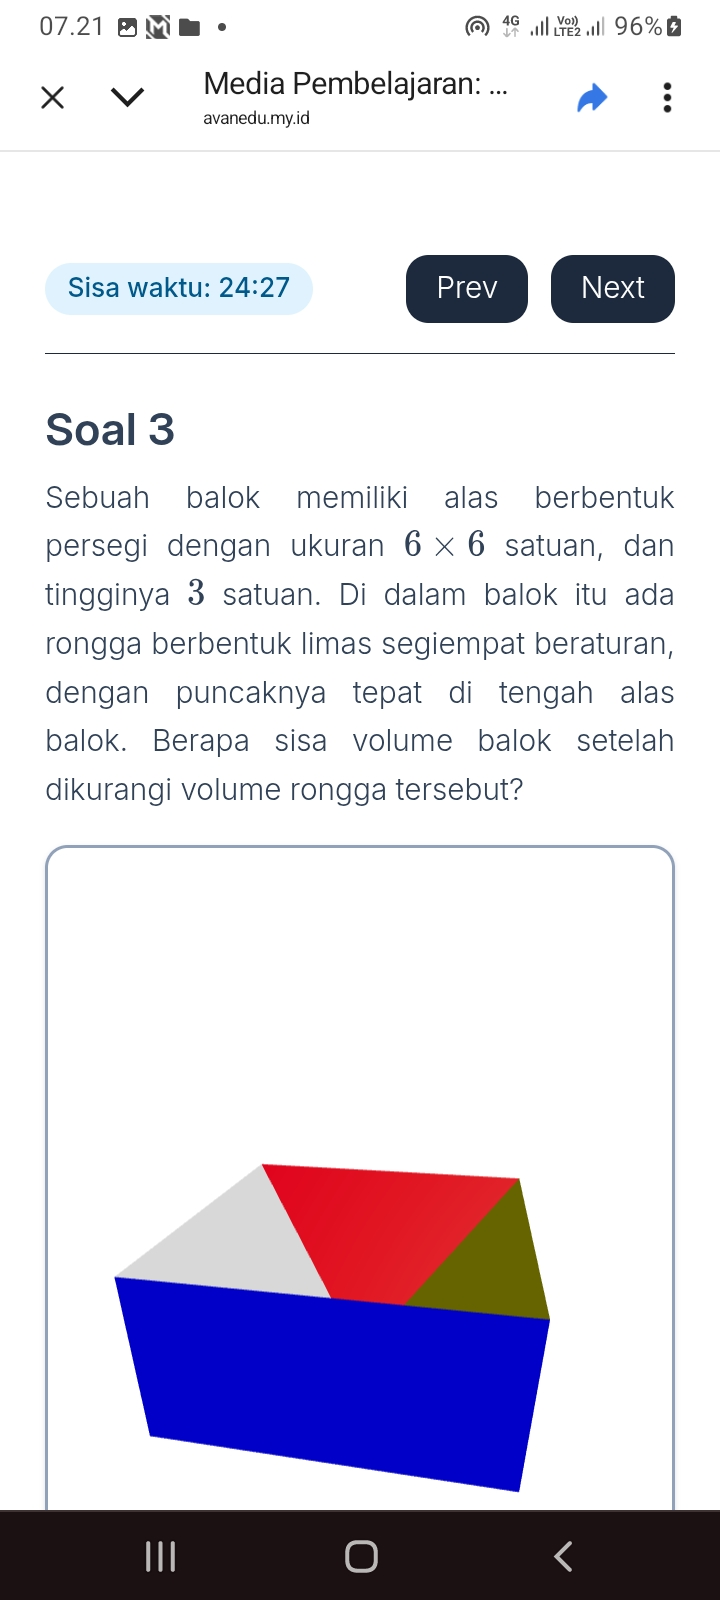
\includegraphics[width=0.25\textwidth]{images/kuis3.jpg}
        \caption{Halaman Kuis}
        \label{fig:kuis}
    \end{figure}
\end{enumerate}